%%%%%%%%%%%%%%%%%%%%%%%%%%%%%%%%%%%%%%%%%%%%%%%%%%%%%%%%%%%%%%%
%% OXFORD THESIS TEMPLATE

% Use this template to produce a standard thesis that meets the Oxford University requirements for DPhil submission
%
% Originally by Keith A. Gillow (gillow@maths.ox.ac.uk), 1997
% Modified by Sam Evans (sam@samuelevansresearch.org), 2007
% Modified by John McManigle (john@oxfordechoes.com), 2015
%
% This version Copyright (c) 2015-2017 John McManigle
%
% Broad permissions are granted to use, modify, and distribute this software
% as specified in the MIT License included in this distribution's LICENSE file.
%

% I've (John) tried to comment this file extensively, so read through it to see how to use the various options.  Remember
% that in LaTeX, any line starting with a % is NOT executed.  Several places below, you have a choice of which line to use
% out of multiple options (eg draft vs final, for PDF vs for binding, etc.)  When you pick one, add a % to the beginning of
% the lines you don't want.


%%%%% CHOOSE PAGE LAYOUT
% The most common choices should be below.  You can also do other things, like replacing "a4paper" with "letterpaper", etc.

% This one will format for two-sided binding (ie left and right pages have mirror margins; blank pages inserted where needed):
\documentclass[a4paper,twoside]{main}
% This one will format for one-sided binding (ie left margin > right margin; no extra blank pages):
%\documentclass[a4paper]{ociamthesis}
% This one will format for PDF output (ie equal margins, no extra blank pages):
%\documentclass[a4paper,nobind]{ociamthesis} 

%%%%% SELECT YOUR DRAFT OPTIONS
% Three options going on here; use in any combination.  But remember to turn the first two off before
% generating a PDF to send to the printer!

% This adds a "DRAFT" footer to every normal page.  (The first page of each chapter is not a "normal" page.)
\fancyfoot[C]{\emph{DRAFT Printed on \today}}  

% This highlights (in blue) corrections marked with (for words) \mccorrect{blah} or (for whole
% paragraphs) \begin{mccorrection} . . . \end{mccorrection}.  This can be useful for sending a PDF of
% your corrected thesis to your examiners for review.  Turn it off, and the blue disappears.
\correctionstrue


%%%%% BIBLIOGRAPHY SETUP
% Note that your bibliography will require some tweaking depending on your department, preferred format, etc.
% The options included below are just very basic "sciencey" and "humanitiesey" options to get started.
% If you've not used LaTeX before, I recommend reading a little about biblatex/biber and getting started with it.
% If you're already a LaTeX pro and are used to natbib or something, modify as necessary.
% Either way, you'll have to choose and configure an appropriate bibliography format...

% The science-type option: numerical in-text citation with references in order of appearance.
\usepackage[style=nature, sorting=none, backend=biber, doi=false, isbn=false]{biblatex}
\newcommand*{\bibtitle}{References}

% The humanities-type option: author-year in-text citation with an alphabetical works cited.
%\usepackage[style=authoryear, sorting=nyt, backend=biber, maxcitenames=2, useprefix, doi=false, isbn=false]{biblatex}
%\newcommand*{\bibtitle}{Works Cited}

% This makes the bibliography left-aligned (not 'justified') and slightly smaller font.
\renewcommand*{\bibfont}{\raggedright\small}

% Change this to the name of your .bib file (usually exported from a citation manager like Zotero or EndNote).
\addbibresource{text/ref_gen_210302.bib}


% Uncomment this if you want equation numbers per section (2.3.12), instead of per chapter (2.18):
%\numberwithin{equation}{subsection}



%%%%% THESIS / TITLE PAGE INFORMATION
% Everybody needs to complete the following:
\title{Regulation of the pancreatic K\textsubscript{ATP} channel}
\author{Samuel Usher}
\college{Green Templeton College}

% Master's candidates who require the alternate title page (with candidate number and word count)
% must also un-comment and complete the following three lines:
%\masterssubmissiontrue
%\candidateno{933516}
%\wordcount{28,815}

% Uncomment the following line if your degree also includes exams (eg most masters):
%\renewcommand{\submittedtext}{Submitted in partial completion of the}
% Your full degree name.  (But remember that DPhils aren't "in" anything.  They're just DPhils.)
\degree{Doctor of Philosophy}
% Term and year of submission, or date if your board requires (eg most masters)
\degreedate{Trinity 2021}


%%%%% YOUR OWN PERSONAL MACROS
% This is a good place to dump your own LaTeX macros as they come up.

% To make text superscripts shortcuts
	\renewcommand{\th}{\textsuperscript{th}} % ex: I won 4\th place
	\newcommand{\nd}{\textsuperscript{nd}}
	\renewcommand{\st}{\textsuperscript{st}}
	\newcommand{\rd}{\textsuperscript{rd}}
	\newcommand{\ATP}{\textsubscript{ATP}}

% To make coloured figure backgrounds and allow for multipanel figures
\usepackage{caption}
\usepackage{subcaption}
\usepackage{mdframed}
\usepackage{lipsum}
\usepackage{xcolor}
\definecolor{bg_figure}{RGB}{239, 235, 233}

\let\originalfigure=\figure
\let\endoriginalfigure=\endfigure

\renewenvironment{figure}[1][]{
  \begin{originalfigure}[#1]
    \begin{mdframed}[linecolor=black!30,backgroundcolor=bg_figure]
}{
    \end{mdframed}
  \end{originalfigure}
}
\DeclareCaptionLabelFormat{bold}{\textbf{#2}}
\DeclareCaptionSubType[Alph]{figure}
\DeclareCaptionSubType[Alph]{subfigure}

\captionsetup[subfigure]{
	position=top,
	labelfont=bf,
	textfont=small,
	singlelinecheck=off,
	justification=raggedright,
	labelformat=simple
	}

\captionsetup[figure]{
	position=bottom,
	labelfont={bf,sc},
	textfont=small,
	justification=justified,
	labelformat=simple,
	subrefformat=bold
	}

% For SI units
\usepackage{siunitx}
\DeclareSIUnit\Molar{M}
\DeclareSIUnit\Calorie{cal}
\DeclareSIUnit\Unit{U}

% For model drawing
\usepackage{tikz}
\usepackage{chemfig}
%%%%% THE ACTUAL DOCUMENT STARTS HERE
\begin{document}



%%%%% CHOOSE YOUR LINE SPACING HERE
% This is the official option.  Use it for your submission copy and library copy:
\setlength{\textbaselineskip}{22pt plus2pt}
% This is closer spacing (about 1.5-spaced) that you might prefer for your personal copies:
%\setlength{\textbaselineskip}{18pt plus2pt minus1pt}

% You can set the spacing here for the roman-numbered pages (acknowledgements, table of contents, etc.)
\setlength{\frontmatterbaselineskip}{17pt plus1pt minus1pt}

% Leave this line alone; it gets things started for the real document.
\setlength{\baselineskip}{\textbaselineskip}


%%%%% CHOOSE YOUR SECTION NUMBERING DEPTH HERE
% You have two choices.  First, how far down are sections numbered?  (Below that, they're named but
% don't get numbers.)  Second, what level of section appears in the table of contents?  These don't have
% to match: you can have numbered sections that don't show up in the ToC, or unnumbered sections that
% do.  Throughout, 0 = chapter; 1 = section; 2 = subsection; 3 = subsubsection, 4 = paragraph...

% The level that gets a number:
\setcounter{secnumdepth}{2}
% The level that shows up in the ToC:
\setcounter{tocdepth}{2}


%%%%% ABSTRACT SEPARATE
% This is used to create the separate, one-page abstract that you are required to hand into the Exam
% Schools.  You can comment it out to generate a PDF for printing or whatnot.
\begin{abstractseparate}
	ATP-sensitive potassium (K\ATP{}) channels are present in many tissues, most notably pancreatic islets and cardiac cells, where they couple the metabolic state of a cell to its electrical activity by regulating the flow of K\textsuperscript{} across the membrane in response to the intracellular ATP/ADP ratio.
K\ATP{} channels are an octameric complex, comprised of four inwardly-rectifying potassium channel (Kir) subunits, each of which is associated with a sulphonylurea receptor (SUR) subunit. 
In pancreatic islets, K\ATP{} channels are formed by Kir6.2 and SUR1.

The physiological regulation of K\ATP{} activity by the ATP/ADP ratio is the summed contribution of activation by Mg-nucleotides binding to SUR1, and inhibition by nucleotides binding to Kir6.2.
Mutations in either Kir6.2 and SUR1 which lead to diseases of insulin secretion are frequently observed to disrupt the nucleotide regulation of the channel.
 % Create an abstract.tex file in the 'text' folder for your abstract.
\end{abstractseparate}


% JEM: Pages are roman numbered from here, though page numbers are invisible until ToC.  This is in
% keeping with most typesetting conventions.
\begin{romanpages}

% Title page is created here
\maketitle

%%%%% DEDICATION -- If you'd like one, un-comment the following.
%\begin{dedication}
%This thesis is dedicated to\\
%someone\\
%for some special reason\\
%\end{dedication}

%%%%% ACKNOWLEDGEMENTS -- Nothing to do here except comment out if you don't want it.
\begin{acknowledgements}
 	First of all, thank you Fran for your endless well of knowledge, and your support and encouragement throughout my time in your lab.
Your enthusiasm for science will continue to inspire me, and I will always be grateful for your patience.
Thank you Mike, for taking on a graduate student who had never patched a cell before and infusing me with your love for ion channels.
I couldn't have asked for a better friend and colleague.

Thank you to the Ashcroft lab, past and present, for your companionship, expertise, and hard work - Raul, Idoia, Natascia, Lizzie, Gregor, Will.
It has been a privilege to work and learn alongside you.
Thank you to the other members of the ion channel journal club for putting up with my ramblings and contributing some of your own.
Harvey, Brad, Max - it's been a pleasure falling back in love with Oxford with you guys.

Thank you Meg for your constant support and for being a shoulder to lean on whenever I have needed it.
Finally, thank you to my family - Mum, Dad, I will never be able to fully express my gratitude for everything you have done to get me here.
\end{acknowledgements}

%%%%% ABSTRACT -- Nothing to do here except comment out if you don't want it.
\begin{abstract}
	ATP-sensitive potassium (K\ATP{}) channels are present in many tissues, most notably pancreatic islets and cardiac cells, where they couple the metabolic state of a cell to its electrical activity by regulating the flow of K\textsuperscript{} across the membrane in response to the intracellular ATP/ADP ratio.
K\ATP{} channels are an octameric complex, comprised of four inwardly-rectifying potassium channel (Kir) subunits, each of which is associated with a sulphonylurea receptor (SUR) subunit. 
In pancreatic islets, K\ATP{} channels are formed by Kir6.2 and SUR1.

The physiological regulation of K\ATP{} activity by the ATP/ADP ratio is the summed contribution of activation by Mg-nucleotides binding to SUR1, and inhibition by nucleotides binding to Kir6.2.
Mutations in either Kir6.2 and SUR1 which lead to diseases of insulin secretion are frequently observed to disrupt the nucleotide regulation of the channel.

\end{abstract}

%%%%% MINI TABLES
% This lays the groundwork for per-chapter, mini tables of contents.  Comment the following line
% (and remove \minitoc from the chapter files) if you don't want this.  Un-comment either of the
% next two lines if you want a per-chapter list of figures or tables.
\dominitoc % include a mini table of contents
%\dominilof  % include a mini list of figures
%\dominilot  % include a mini list of tables

% This aligns the bottom of the text of each page.  It generally makes things look better.
\flushbottom

% This is where the whole-document ToC appears:
\tableofcontents

\listoffigures
	\mtcaddchapter
% \mtcaddchapter is needed when adding a non-chapter (but chapter-like) entity to avoid confusing minitoc

% Uncomment to generate a list of tables:
%\listoftables
%	\mtcaddchapter

%%%%% LIST OF ABBREVIATIONS
% This example includes a list of abbreviations.  Look at text/abbreviations.tex to see how that file is
% formatted.  The template can handle any kind of list though, so this might be a good place for a
% glossary, etc.
\graphicspath{{figures/appendix/}}

\begin{mclistof}{List of Abbreviations}{3.2cm}

\item[ABC] ATP-binding cassette

\item[ADP] Adenosine diphosphate

\item[ATP] Adenosine triphosphate

\item[ANAP] L-3-(6-acetylnaphthalen-2-ylamino)-2-aminopropionic acid

\item[CFTR] Cystic fibrosis transmembrane conductance regulator

\item[Cryo-EM] Cryo-electron microscopy

\item[EC\textsubscript{50}] Half maximal effective concentration

\item[ER] Endoplasmic reticulum

\item[FRET] F\"{o}rster resonance energy transfer

\item[GFP] Green fluorescent protein

\item[HA] Human influenza hemagglutinin

\item[HEK293T] Human embryonic kidney 293 cells containing the SV40 T-antigen

\item[IC\textsubscript{50}] Half maximal inhibitory concentration

\item[K\ATP{} channel] ATP-sensitive potassium channel

\item[Kir] Inward rectifier potassium channel

\item[L0] Loop zero

\item[LOO-CV] Leave-one-out cross-validation

\item[mO] mOrange fluorescent protein

\item[MWC] Monod-Wyman-Changeaux

\item[NBD] Nucleotide binding domain

\item[PCF] Patch-clamp fluorometry

\item[PDB] Protein data bank

\item[PIP\textsubscript{2}] Phosphatidylinositol 4,5-bisphosphate

\item[$P_O$] Open probability

\item[SUR] Sulphonylurea receptor

\item[TEA\textsuperscript{+}] Triethylammonium ion

\item[TMD] Transmembrane domain

\item[TNP-ADP] Trinitrophenyl adenosine diphosphate

\item[TNP-ATP] Trinitrophenyl adenosine triphosphate

\item[UAA] Unnatural amino acid

\item[WT] Wild-type

\end{mclistof}

\begin{figure}[h]
	\centering
	\begin{subfigure}[t]{0.45\textwidth}
		\caption{}\label{ch0fig:kir_constructs}
		\centering
		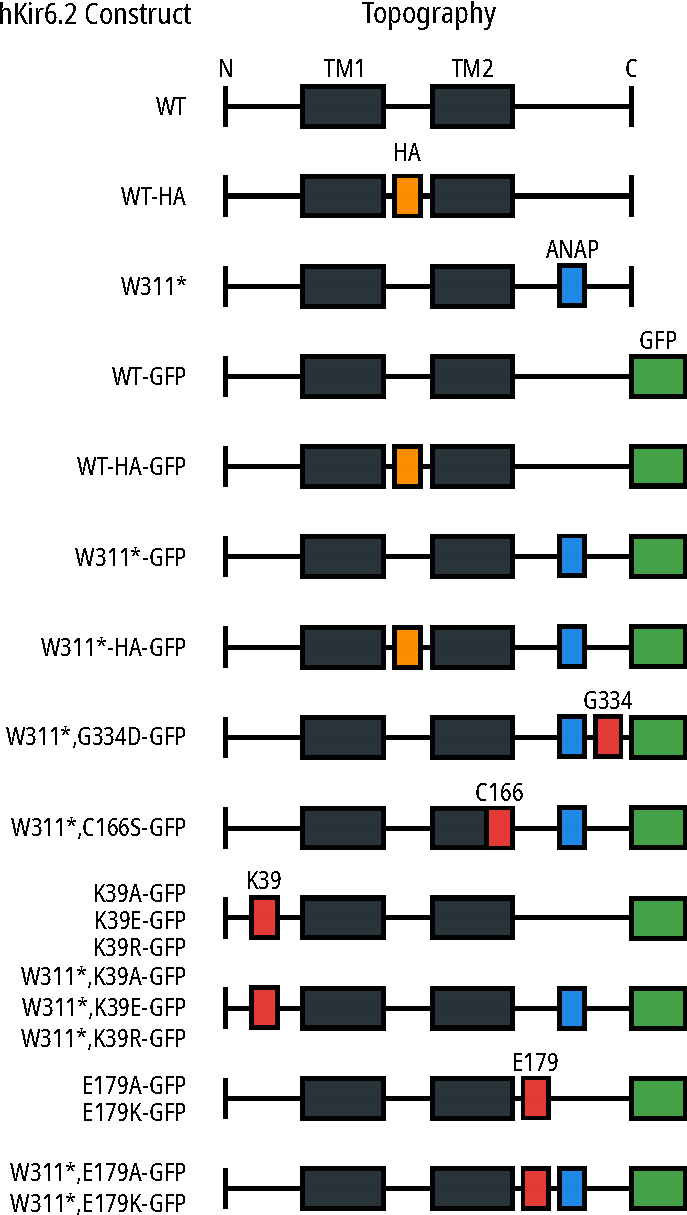
\includegraphics[width=\textwidth]{kir_constructs.pdf}
	\end{subfigure}
	\hfill
	\begin{subfigure}[t]{0.45\textwidth}
		\caption{}\label{ch0fig:sur_constructs}
		\centering
		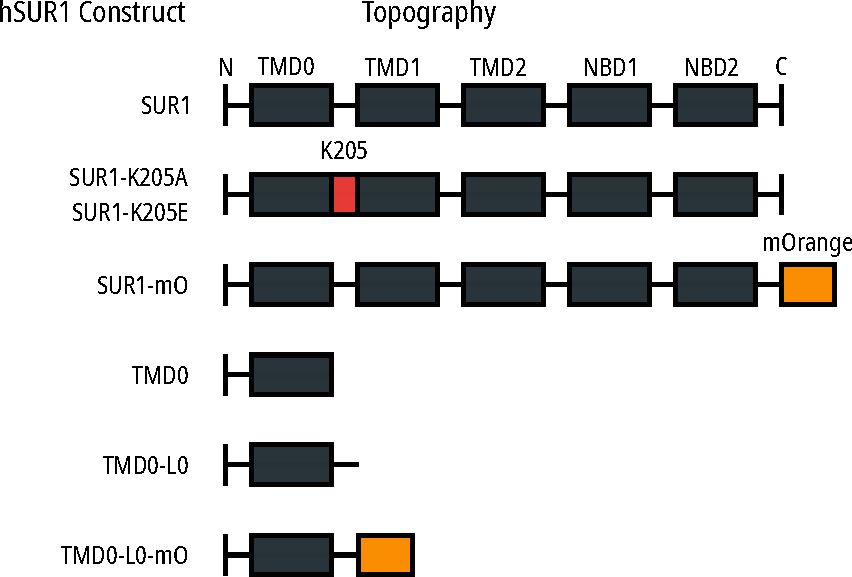
\includegraphics[width=\textwidth]{sur_constructs.pdf}
	\end{subfigure}
	\caption[hKir6.2 and hSUR1 constructs and their abbreviations]{
	}\label{ch0fig:constructs}
\end{figure}

% The Roman pages, like the Roman Empire, must come to its inevitable close.
\end{romanpages}


%%%%% CHAPTERS
% Add or remove any chapters you'd like here, by file name (excluding '.tex'):
\flushbottom
\chapter{\label{ch:1-intro}Introduction} 

\graphicspath{{figures/ch1/}}

\minitoc

\section{General introduction}

\section{Pancreatic islets and the \textgreek{b}-cell}

Pancreatic islets are endocrine cells which are responsible for maintaining glucose homeostasis.
There are roughly one million islets in a human pancreas, constituting 1-2\% of the total pancreatic mass.
Islets consist of three principal cell types; insulin secreting \textgreek{b}-cells, glucagon secreting \textgreek{a}-cells and somatostatin secreting \textgreek{D}-cells.
Islets respond to increases in blood glucose by releasing insulin, which acts on peripheral tissues to increase glucose uptake and reduce blood glucose levels.
Conversely, decreases in blood glucose leads to the release of glucagon, which acts on those tissues to stimulate glucose production and increase blood glucose.

\section{Architecture of the pancreatic K\ATP{} channel}

ATP-sensitive potassium (K\ATP{}) channels are present in many tissues, where they couple the metabolic state of a cell to its electrical activity by regulating the flow of K\textsuperscript{+} across the membrane.
K\ATP{} channels are an octameric complex, comprised of four inwardly-rectifying potassium channel subunits (Kir6.1 or Kir6.2), each of which is associated with a sulphonylurea receptor subunit (SUR1, SUR2A or SUR2B).
In pancreatic \textgreek{b}-cells, the K\ATP{} channel isoform is composed of Kir6.2 and SUR1.
Together, Kir6.2 and SUR1 form a complex nearly a megadalton in size and over 15 nanometres across (Figure \ref{ch1fig:katp_cartoon}, \ref{ch1fig:sur_topdown}).

Inwardly-rectifying potassium channels are so named because they allow K\textsuperscript{+} to flow more easily into the cell than out of it (Figure \ref{ch1fig:rectification}).
This phenomenon is a consequence of voltage-dependent pore blockade by intracellular divalent cations (especially Mg\textsuperscript{2+}) and polyamines.
At depolarising membrane potentials, blockers are driven into the pore and K\textsuperscript{+} current is blocked, while at hyperpolarising potentials the blockers and cleared and K\textsuperscript{+} current can flow.
Strongly rectifying Kir channels display drastically reduced conductance at potentials more positive than the K\textsuperscript{+} reversal potential.
In contrast, Kir6.2 is a weak rectifier, and allows substantial current to flow at more positive potentials.

In addition to voltage, Kir6.2 is regulated by two endogenous ligands; 
phosphatidylinositol 4,5-bisphosphate (PIP\textsubscript{2}) and adenine nucleotides (Figure \ref{ch1fig:kir_struct}).
The binding of adenine nucleotides to Kir6.2 leads to closure of the channel pore, while the binding of PIP\textsubscript{2} promotes the opening of the pore (Figure \ref{ch1fig:shyng_trace}).
Activation by PIP\textsubscript{2} is a mechanism common to the whole Kir family, wherease inhibition by nucleotides is unique to the Kir6 subfamily.

\begin{figure}[h]
	\centering
	\begin{subfigure}[t]{0.5\textwidth}
		\caption{}\label{ch1fig:rectification}
		\centering
		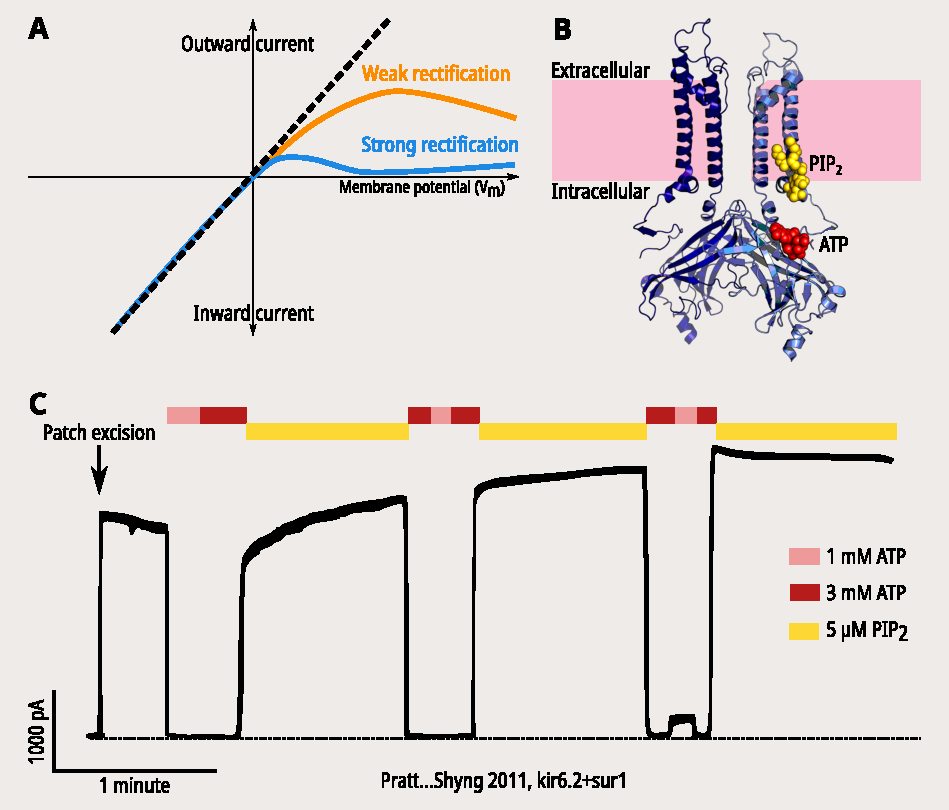
\includegraphics[width=\textwidth]{rectification.pdf}
	\end{subfigure}
	\hfill
	\begin{subfigure}[t]{0.4\textwidth}
		\caption{}\label{ch1fig:kir_struct}
		\centering
		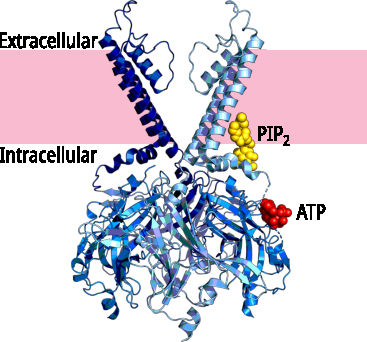
\includegraphics[width=\textwidth]{kir_structure.pdf}
	\end{subfigure}
	\vfill
	\begin{subfigure}[t]{0.9\textwidth}
		\caption{}\label{ch1fig:shyng_trace}
		\centering
		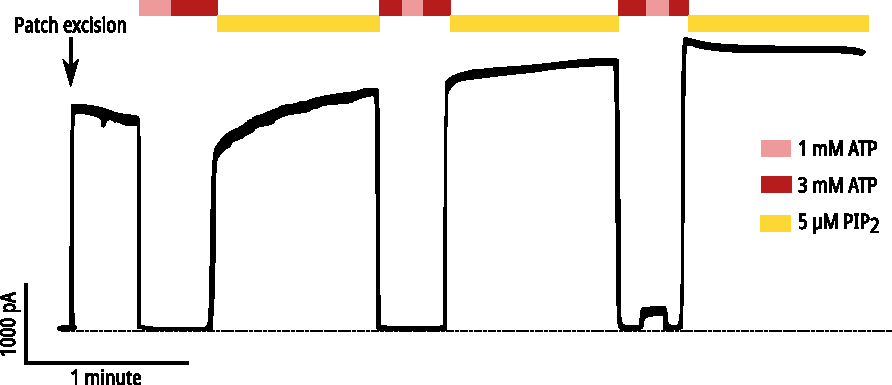
\includegraphics[width=\textwidth]{shyng_atp_pip_trace.pdf}
	\end{subfigure}
	\caption[Structure of Kir6.2]{
		\subref{ch1fig:rectification} Current-voltage plot demonstrating inward rectification of Kir channels.
		Here, the reversal potential of potassium (\textit{E\textsubscript{K}}) is set to zero, i.e. there is an equal concentration of K\textsuperscript{+} on each side of the membrane.
		Weak rectifiers such as Kir6.2 exhibit only a weak voltage dependent decline in conductance (visualised as a departure from the dashed line of an ideal conductor).
		(Kind of adapted from Handbook of Ion Channels).
		\subref{ch1fig:kir_struct} Cryo-EM structure of Kir6.2 (PDB \#6BAA) captured with ATP bound (red) and with the proposed binding position of PIP\textsubscript{2} visualised by alignment of the channel with the X-ray structure of Kir2.2 solved in compex with a short-chain dioctanoyl (diC8) PIP\textsubscript{2} (PDB \#6C3I).
		The plasma membrane is shown in pink.
		(Kind of adapted from Mike's JGP review).
		\subref{ch1fig:shyng_trace} Macroscopic currents from Kir6.2 channels coexpressed with SUR1 in excised patches from cultured cells, adapted from (Pratt/Shyng, 2011).
		Perfusion of ATP or PIP\textsubscript{2} is indicated by coloured bars, and demonstrates the contrasting effects of these two ligands on channel activity.
	}
	\label{ch1fig:kir_breakdown}
\end{figure}

SUR1 is a member of the ATP-binding cassette (ABC) family of transporters.
While other ABC proteins transport substrate across the membrane, SUR1 does not appear to do so; instead it acts to modulate the function of its associated ion channel.
The cystic fibrosis transmembrane conductance regulator (CFTR) is another member of the ABC family, and is an ion channel in its own right, capable of conducting chloride across the membrane.
Like other ABC proteins, SUR1 contains two sets of transmembrane domains (TMD1 and TMD2) and two cytosolic nucleotide binding domains (NBD1 and NBD2).
Unique to SUR is the presence of an additional transmembrane domain (TMD0) N-terminal to the core of the protein, and this domain forms the primary contact between SUR1 and Kir6.2.

The NBDs of ABC transporters are highly conserved, and consist of two subdomains: a larger RecA-like subdomain found in other P-loop ATPases, and a smaller \textgreek{a}-helical subdomain which is unique to ABC transporters.
There are three key structural motifs present in these subdomains: the RecA-like subdomain contains the Walker A (W\textsubscript{A}) and B (W\textsubscript{B}) motifs, while the \textgreek{a}-helical subdomain contains the ABC signature motif (typically LSGGQ).

The two domains come together to form an antiparallel dimer with two nucleotide binding sites (NBS1 and NBS2) at the interface, such that NBS1 is formed from the W\textsubscript{A} and W\textsubscript{B} motifs of NBD1 and the signature motif from NBD2, whereas NBS2 is formed from the W\textsubscript{A} and W\textsubscript{B} motifs of NBD2 and the signature motif from NBD1.
NBS2, also known as the consensus site as it is more similar in sequence to other ABC family members, is catalytically competent and able to hydrolyse ATP.
In contrast, NBS1 is the degenerate site, with a less conserved sequence and an inability to catalyse hydrolysis of ATP.

\begin{figure}[h]
	\centering
	\begin{subfigure}[t]{0.4\textwidth}
		\caption{}\label{ch1fig:sur_struct}
		\centering
		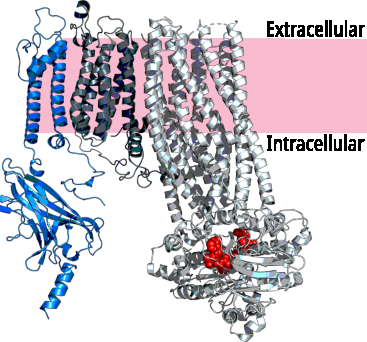
\includegraphics[width=\textwidth]{sur_structure.pdf}
	\end{subfigure}
	\hfill
	\begin{subfigure}[t]{0.5\textwidth}
		\caption{}\label{ch1fig:nbd_struct}
		\centering
		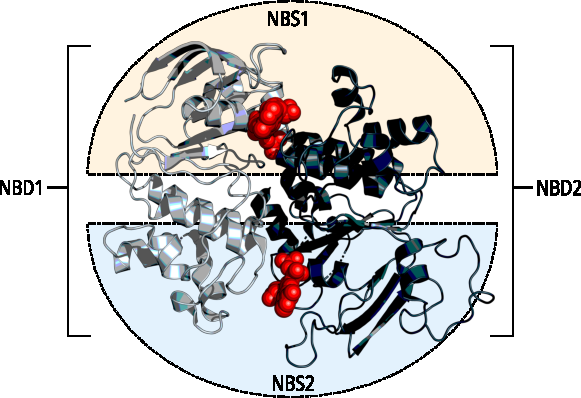
\includegraphics[width=\textwidth]{nbd_structure.pdf}
	\end{subfigure}
	\caption[Structure of SUR1]{
		\subref{ch1fig:sur_struct} Cryo-EM structure of SUR1 captured with a nucleotide (shown in red) bound at each NBS (PDB \#6C3P).
		A single SUR1 subunit is shown, with TMD1 and TMD2 in white and TMD0 in grey.
		A single Kir6.2 subunit is also shown in blue to show the interface between subunits.
		The plasma membrane is displayed in pink.
		\subref{ch1fig:nbd_struct} Top-down view of the NBDs from the same cryo-EM structure.
		NBD1 is on the left in white, NBD2 is on the right in grey, and the two NBSs are higlighted; NBS1 in orange and NBS2 in blue.
		Adapted from Mikes JGP review.
	}
\end{figure}

\section{Ligand-independent regulation of the pancreatic K\ATP{} channel}

\subsection{Assembly and trafficking}

Biogenesis of K\ATP{} channels occurs in the endoplasmic reticulum (ER), and is an important checkpoint in determining surface expression and channel stoichiometry \cite{zerangue_new_1999-1, martin_pharmacological_2013}.
The precise nature of the events which occur between subunit translation and insertion of octameric K\ATP{} into the cell membrane are not fully mapped out, but studies have highlighted some important quality control steps in this process which regulate K\ATP{} channel expression.
When Kir6.2 or SUR1 are expressed alone in heterologous systems, they are retained in the ER \cite{zerangue_new_1999-1}.
This mechanism is achieved through the exposure of a three amino acid ER-retention motif (RKR) in the cytoplasmic domains of both Kir6.2 and SUR1.
Only upon complete assembly of the channel complex are the RKR motifs masked, allowing forward trafficking of K\ATP{} to the cell surface.
Deletion of the RKR motif \cite{tucker_truncation_1997}, or mutation of the motif to AAA \cite{zerangue_new_1999-1}, results in unregulated surface expression of individual subunits and/or partially assembled channel complexes.
Addition of a GFP label to the C-terminus of Kir6.2 is also sufficient to allow trafficking of subunits to the cell surface in the absence of SUR1 \cite{john_sulphonylurea_1998-1}.

In addition to the RKR motif, there are two N-linked glycosylation sites on SUR1 (N10 and N1050) which are required for cell surface expression \cite{conti_membrane_2002}.
Mutation of these sites to glutamines results in retention in the ER and drastically reduced expression of K\ATP{} on the cell surface.
This mechanism is thought to be separate to that for the ER-retention motif, as mutation of RKR to AAA is not sufficient to drive surface expression of the glycosylation mutants \cite{conti_membrane_2002}.

A putatitive third site of trafficking regulation is in the C-terminus of SUR1.
Mutation or deletion of a dileucine motif 16 amino acids distal to the C-terminal of SUR1 results in reduced surface expression of K\ATP{} channels in COSm6 cells \cite{sharma_c_1999}.
This reduction in expression is not rescued by C-terminal truncation of Kir6.2, indicating that this result is not due to masking of the RKR retention motif.
The dileucines are therefore suggested to promote forward trafficking of assembled channel complexes to the cell membrane \cite{sharma_c_1999}.
Expression of K\ATP{} channels expressed in \textit{Xenopus} oocytes is also dramatically reduced by truncation of the C-terminal 42 amino acids of SUR1 \cite{vedovato_role_2018}.
However, longer deletions of the SUR1 C-terminus did not reduce surface expression of channels in HEK293 cells \cite{giblin_cytoplasmic_2002}, and other modifications of the SUR1 C-terminus do not exhibit effects on surface expression \cite{schwappach_molecular_2000}.
In fact, a splice variant of SUR1 missing the entirety of the NBD2 domain (truncated at residue 1355) was found to successfully traffic to the membrane of insulin-secreting \textgreek{b}-cell line MIN6 cells \cite{sakura_altered_1999-1}.
The precise role of the dileucine motif remains unclear, and is potentially confounded by the use of expression system \cite{giblin_cytoplasmic_2002, martin_pharmacological_2013}

Failure of the channel complex to pass these three checkpoints results in ER-associated degradation (ERAD), a common pathway shared by most membrane and secretory proteins \cite{bonifacino_ubiquitin_1998, yan_role_2005}.
Both SUR1 and Kir6.2 are substrates for polyubiquitination, both when heterologously expressed and in INS-1 cells \cite{yan_role_2005}.
Application of proteasome inhibitors both reduces the rate of degradation for Kir6.2 and SUR1, and increases the surface expression of K\ATP{} channels by increasing their biogenesis efficiency \cite{yan_role_2005}.

The surface expression of K\ATP{} channels is therefore controlled by a variety of different quality control mechanism to ensure that only correctly assembled octameric channel complexes reach the cell membrane.
Mutations which lead to defects in assembly and trafficking are therefore a common cause of congenital hyperinsulinemia (HI).
These mutations are found throughout both Kir6.2 and SUR1, although they are more commonly found in SUR1 \cite{martin_pharmacological_2013}.

Interestingly, sulphonylureas are able to act as pharmacological chaperones and rescue surface expression of several mutations which would otherwise not traffic to the cell surface \cite{yan_sulfonylureas_2004, yan_sulfonylureas_2006, yan_congenital_2007, yan_congenital_2007-1, martin_pharmacological_2016}.
Sulphonylureas bind directly to the channel during biogenesis, as mutation of residues in SUR1 which are critical for sulphonylurea binding abolished or reduced the effectiveness of expression rescue \cite{yan_sulfonylureas_2006}.
Pharmacological chaperoning requires full assembly of the channel complex, as the presence of Kir6.2 was required to rescue expression of trafficking mutants even when the SUR1 RKR motif was mutated to AAA \cite{yan_sulfonylureas_2006}.
In addition, reducing the temperature at which cells are cultured can rescue some trafficking defects \cite{yang_low_2005}.

\begin{figure}[h]
	\centering
	\begin{subfigure}[t]{0.9\textwidth}
		\caption{}\label{ch1fig:katp_cartoon}
		\centering
		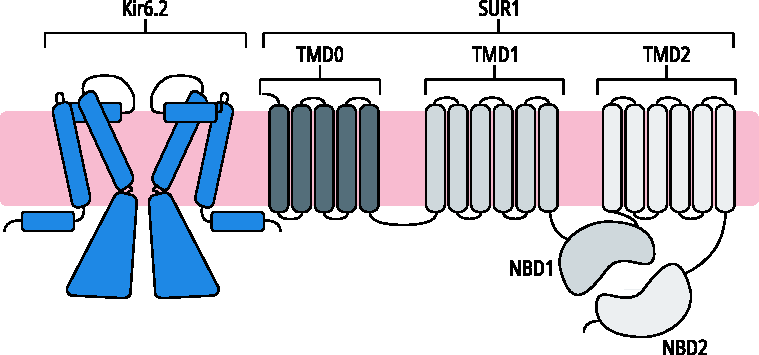
\includegraphics[width=\textwidth]{katp_cartoon.pdf}
	\end{subfigure}
	\vfill
	\begin{subfigure}[t]{0.45\textwidth}
		\caption{}\label{ch1fig:sur_topdown}
		\centering
		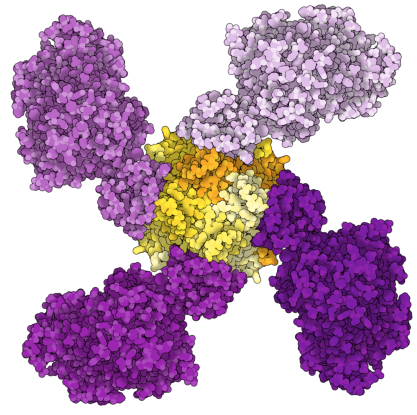
\includegraphics[width=\textwidth]{sur_topdown_propellor.pdf}
	\end{subfigure}
	\hfill
	\begin{subfigure}[t]{0.45\textwidth}
		\caption{}\label{ch1fig:sur_ctd}
		\centering
		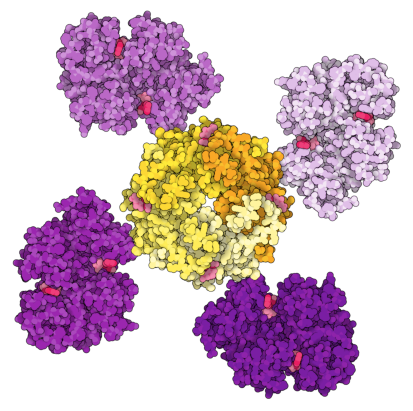
\includegraphics[width=\textwidth]{sur_topdown_ctd_propellor.pdf}
	\end{subfigure}
	\caption[K\ATP{} architecture and nucleotide regulation]{
		\subref{ch1fig:katp_cartoon} Membrane topology of the K\ATP{} channel shown with two Kir6.2 subunits and one SUR1 subunit.
		\subref{ch1fig:sur_topdown} Top-down view of a cryo-EM structure of the K\ATP{} channel (PDB \# 6C3P) solved with nucleotides bound at each of the three canonical binding sites.
		Each SUR1 subunit is shown in a shade of purple, and each Kir6.2 subunit is shown in a shade of orange.
		\subref{ch1fig:sur_ctd} The same view of the structure shown to the left, but with the transmembrane domains removed to reveal the cytoplasmic domains of each subunit only.
		The nucleotides bound to the channel are shown in red.
	}
\end{figure}

\subsection{Regulation of intrinsic gating}

In the absence of nucleotides, K\ATP{} channels are spontaneously active.
This can be seen at a macroscopic level in excised patches.
Upon excision of a patch from a cell membrane containing K\ATP{} channels, the magnitude of current dramatically increases when voltage is applied (Figure \ref{ch1fig:shyng_trace}), reflecting the relief from inhibition of cytoplasmic nucleotides.
While this macroscopic time course is smooth and graded, it consists of hundreds or thousands of individual channels which exhibit binary behaviour; switching between a nonconducting closed state and a conducting open state \ref{hille_ion_2001}.
The summed activity of these individual channels constitutes the large currents observed in macroscopic excised patches.

Single K\ATP{} channels exhibit bursts of brief openings, separated by long interburst closures \cite{alekseev_ligand-insensitive_1998, babenko_two_1999, li_open_2002, proks_modeling_2009}.
Thus, the open probability ($P_O$) of the channel is determined both by the kinetics of the burst (open and closed durations within a burst) and the duration of the long interburst closures.
The intrinsic gating of K\ATP{} can therefore be separated into two separate 'gating' processes; fast (responsible for intraburst closures) and slow (responsible for interburst closures).
While it is helpful to distinguish between fast and slow gating processes to characterise channel regulation, doing so does not require the existence of separate structural gates \cite{proks_modeling_2009, hille_ion_2001}.

Gating is a property intrinsic to Kir6.2, which is able to open and close in the absence of SUR1 \cite{tucker_truncation_1997, enkvetchakul_kinetic_2000-1} (Figure \ref{ch1fig:singles_sur}); albeit with very different kinetic properties which will be discussed later.
The open and intraburst closed time of single channels is dependent on the electrochemical gradient across the cell membrane, otherwise called the K\textsuperscript{+} driving force \cite{benz_characterization_1998}.
As the name implies, the electrochemical gradient depends on two things: the voltage across the membrane, and the K\textsuperscript{+} concentration gradient.
Increasing hyperpolarisation decreases the amount of time channels remain in the open state and increases the amount of time channels remain in the closed state within bursts \cite{alekseev_burst_1997, trapp_molecular_1998-1}.
This is a characteristic feature shared by other inwardly-rectifying K\textsuperscript{+} channels \cite{sakmann_voltage-dependent_1984, alekseev_burst_1997}.
In addition, altering the  K\textsuperscript{+} gradient across the membrane by changing the K\textsuperscript{+} concentration in the pipette or bath solution has the same effect on fast gating kinetics \cite{zilberter_gating_1988, benz_characterization_1998}.
As the driving force for K\textsuperscript{+} increases, the open lifetime of the K\ATP{} channel decreases.
This is in contrast to other K\textsuperscript{+} channels such as K\textsubscript{V}2.1, which exhibits the opposite relationship \cite{chapman_allosteric_2006}.

There are a number of domains within Kir6.2 that regulate the intrinsic gating of the channel.
Firstly, the P-loop is a conserved feature across K\textsuperscript{+} channels (amongst others) \cite{kuang_structure_2015}.
In Kir channels, the P-loop connects the two transmembrane domains, and dips into the plasma membrane to form the K\textsuperscript{+} selectivity filter.
While the P-loop is broadly conserved between Kir family members, there are key residues which differ.
Notably, the K\textsuperscript{+} selectivity filter signature sequence (TxGYG) is identical across all other Kir subtypes (TIGYG), but in Kir6.2 the tyrosine is replaced by a phenylalanine at position 133 (TIGFG), a feature shared only by eag-like K\textsuperscript{+} channels \cite{heginbotham_mutations_1994}.
Another particularly interesting residue is V127, which is unique to Kir6.1 and Kir6.2 within the Kir family - all other Kir channels posess a threonine at this location \cite{proks_mutations_2001}.

\citeauthor{proks_mutations_2001} investigated a range of substitutions at these two residues.
Mutation of V127 to the conserved threonine (V127T) dramatically increases the open time of K\ATP{}, while also increasing the intraburst closed time.
There is also some suggestion of an additional open state existing in this mutant construct, evidenced by the appearance of a second peak in the open time histograms.
Mutation of F133 to the conserved tyrosine (F133Y) did not produce expression of functional channels; however combining the two mutations (V127T,F133Y) resulted in functional channels with a further increase in the open time when compared to the single mutant V127T.
In addition, substitutions at other residues in the P-loop of Kir6.2 leads to a range of effects on the intraburst kinetics of K\ATP{}.
Crucially, none of the substitutions affected the slow gating of the channel; i.e. burst duration and interburst closed times remained similar despite the varied alterations in the intraburst kinetics.
\citeauthor{proks_mutations_2001} concluded that the P-loop is instrumental in regulating the fast gating of K\ATP{}, and suggested that the lack of correlation between perturbations of inter- and intra-burst kinetics is evidence for independence between the fast and slow gating processes.
(I haven't mentioned the correlated decrease in conductance associated with these mutations - need to think more about how this ties in with the regulation of open time by driving force).

Other domains of Kir6.2 are involved in the regulation of slow gating.
The cytosolic end of the second transmembrane domain of Kir6.2 has been implicated in regulation of K\ATP{} slow gating by a number of mutational studies \cite{shyng_control_1997, tucker_molecular_1998, trapp_molecular_1998-1, loussouarn_structure_2000}.
Substitution of C166 with a more bulky or hydrophobic residue dramatically reduces the frequency of the channel entering the long, closed interburst state, and increases the open time of the channel in the bursts \cite{trapp_molecular_1998-1}.
However, no effect is seen on the length of the intraburst closed times, which is additional evidence for the independence of the fast and slow gating processes.
Substitutions at N160 \cite{shyng_control_1997}, L164 \cite{tammaro_kir62_2008}, I167 \cite{tucker_molecular_1998}, and T171 \cite{tucker_molecular_1998, drain_katp_1998} also increase channel open time and decrease the rate of entry into the interburst closed state, further implicating this region of Kir6.2 in modulating the slow gating of K\ATP{}.

The slide-helix of Kir6.2 is the interface between the transmembrane domain and the cytoplasmic domain, and mutations in this region result in changes in the single channel kinetics and $P_O$ of K\ATP{} \cite{proks_molecular_2004, koster_dend_2008, mannikko_interaction_2010, li_decomposition_2013,cooper_conserved_2017}.
Mutations examined at the single channel level show changes in burst duration \cite{proks_molecular_2004, koster_dend_2008, mannikko_interaction_2010} but unaltered intraburst kinetics.
Interpretation of the mechanism underlying these single channel kinetics alterations is complicated by the proximity of this region of Kir6.2 to the putative PIP\textsubscript{2} binding site \cite{pipatpolkai_evaluating_2020}.
Perturbations of this region could be affecting intrinsic gating directly, or indirectly by altering PIP\textsubscript{2} regulation, both of which would lead to changes in slow gating.

While Kir6.2 is able to gate intrinsically when expressed alone, coassembly with SUR1 alters the intrinsic gating of the channel in a number of ways.
Compared to the single channel kinetics of Kir6.2\textgreek{D}C or Kir6.2-GFP alone, coexpression of Kir6.2 with SUR1 increases the open time of the channel within the bursts, and increases their duration, while the intraburst closed times are unaffected \cite{trapp_molecular_1998-1, john_sulphonylurea_1998-1, chan_n-terminal_2003-1}.
This suggests that interactions of SUR1 with Kir6.2 serve to regulate the slow gating of the channel, rather than the fast gating.
The mechanisms by which SUR1 regulates intrinsic gating of the K\ATP{} channel are complex and not yet fully understood.
Structurally, the primary contacts between the two subunits are formed between the N-terminus and first transmembrane domain of Kir6.2 and TMD0 and L0 of SUR1 (Figure \ref{ch1fig:sur_struct}) \cite{martin_anti-diabetic_2017, lee_molecular_2017-1, li_structure_2017-1}.
The contributions of the interactions of these regions have been studied in a variety of ways.

\begin{figure}[h]
	\centering
	\begin{subfigure}[t]{0.45\textwidth}
		\caption{}\label{ch1fig:singles_sur}
		\centering
		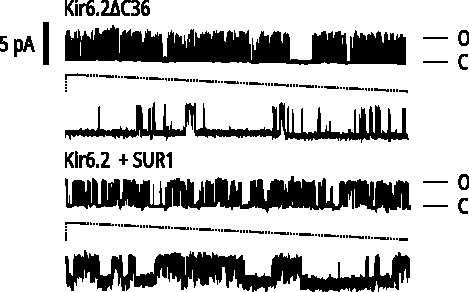
\includegraphics[width=\textwidth]{single_traces_sur.pdf}
	\end{subfigure}
	\hfill
	\begin{subfigure}[t]{0.45\textwidth}
		\caption{}\label{ch1fig:singles_tmd0}
		\centering
		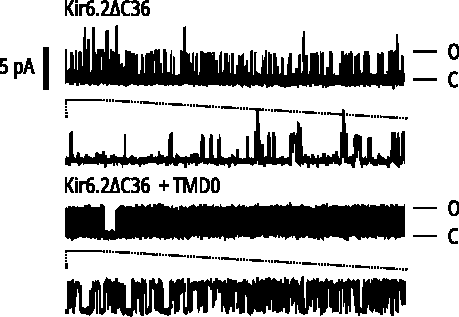
\includegraphics[width=\textwidth]{single_traces_tmd0.pdf}
	\end{subfigure}
	\vfill
	\begin{subfigure}[t]{0.45\textwidth}
		\caption{}\label{ch1fig:intrinsic_diagram}
		\centering
		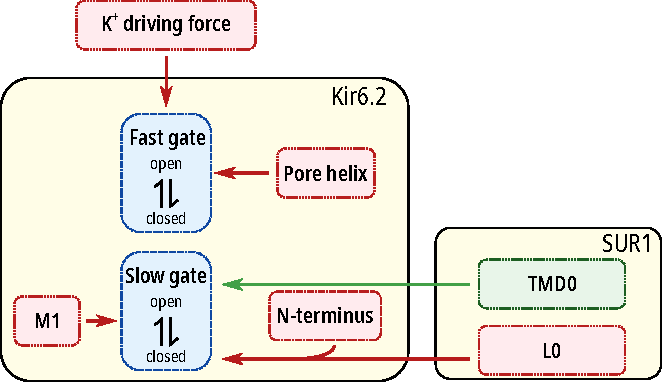
\includegraphics[width=\textwidth]{regulation_diagram_2.pdf}
	\end{subfigure}
	\hfill
	\begin{subfigure}[t]{0.45\textwidth}
		\caption{}\label{ch1fig:sur_shift}
		\centering
		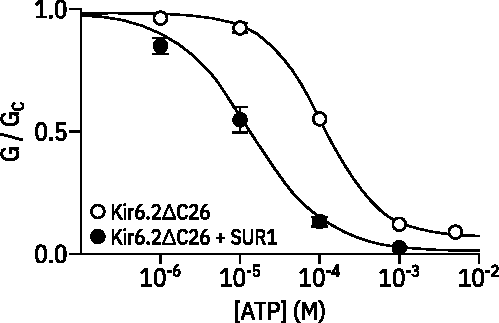
\includegraphics[width=\textwidth]{tucker_sur_shift.pdf}
	\end{subfigure}
	\caption[SUR1 modulates Kir6.2 gating]{
		\subref{ch1fig:singles_sur} Single channel recordings of excised patches from cultured cells either expressing Kir6.2 alone with the C-terminal 36 amino acids truncated (Kir6.2\textgreek{D}C36) or coexpressing wild-type Kir6.2 with SUR1.
		Adapted from (Enkvetchakul/Nichols, 2000).
		\subref{ch1fig:singles_tmd0} Single channel recordings of excised patches from cultured cells either expressing Kir6.2\textgreek{D}C36 alone or coexpressing Kir6.2\textgreek{D}C36 with the TMD0 region of SUR1.
		Adapted from (Pratt/Shyng, 2011).
		In both panels, currents were recorded in symmetrical 140 mM K\textsuperscript{+} at a membrane potential of -50 mV and openings are displayed as upward deflections.
		Note that the timescales differ slightly between panels as traces are from two separate papers.
		\subref{ch1fig:intrinsic_diagram} The intrinsic open-closed equilibrium of the pancreatic K\ATP{} channel pore is regulated by the K\textsuperscript{+} driving force and by the presence of different SUR1 domains.
		\subref{ch1fig:sur_shift} Concentration-response relationship of ATP from macroscopic currents excised from \textit{Xenopus} oocytes injected with either Kir6.2\textgreek{D}C26 mRNA alone (open circles), or a mixture of Kir6.2\textgreek{D}C26 and SUR1 mRNAs (closed circles).
		Response is given as the fraction of the slope conductance (G) remaining during exposure to ATP.
		Adapted from (Tucker/Ashcroft, 1997).
	}
\end{figure}

\citeauthor{babenko_two_1999} constructed a series of SUR1/SUR2A chimeras and characterised the changes in single channel kinetics that resulted from swapping different domains between the two isoforms of SUR.
They found that Kir6.2+SUR2A channels exhibited a far higher single channel $P_O$ than Kir6.2+SUR1 channels (0.91 and 0.64 respectively).
This difference could be attributed to increased burst durations and decreased interburst periods, while fast gating is indistinguishable.
They found that a chimerical construct replacing the N-terminal 291 amino acids of SUR1 with those of SUR2A was sufficient to recapitulate the single channel kinetics of full-length SUR2A, suggesting that this region is critical for specifying the intrinsic gating of K\ATP{}.

Later work established that truncations of SUR1 to TMD0 or TMD0-L0 fragments allowed expression of "mini-K\ATP{}" channels at the cell membrane \cite{babenko_sur_2003, chan_n-terminal_2003, fang_n-terminal_2006}.
The first two studies showed that expression of Kir6.2 with TMD0 alone (residues 1-195 or 1-196 of SUR1) essentially recapitulates the intrinsic gating characteristics of Kir6.2 expressed with full-length SUR1, restoring the increased open time duration and burst duration as compared to expression of Kir6.2 alone \cite{babenko_sur_2003, chan_n-terminal_2003}.
\citeauthor{fang_n-terminal_2006} later found that in their hands, mini-K\ATP{} channels formed from Kir6.2\textgreek{D}C and SUR1-TMD0 were similar to full-length K\ATP{} but they consistently observed differences in the burst durations.
This discrepancy may be, at least in part, due to differences in the heterologous expression system (COSm6 cells in \cite{babenko_sur_2003}, \textit{Xenopus} oocytes in \cite{fang_n-terminal_2006}).
Otherwise, the remaining difference between K\ATP{} and mini-K\ATP{} channels could either be due to differences in structural interactions due to the truncation, or could implicate a role for the ABC core domain in regulating slow gating \cite{fang_n-terminal_2006}.

Increasing the length of the SUR1 fragment to include the first section of the L0 linker (residues 1-232 of SUR1) results in a nearly constitutively open channel, with dramatically increased open time duration and few observable interburst closures \cite{babenko_sur_2003}.
The resulting $P_O$ of 0.93 reflects a near saturation of the slow gating process; as without changes to the fast gating there can be limited further increases in $P_O$ due to the flickery closure.
Increasing the length of the L0 linker included in the SUR1 truncation fragment results in a progressive decrease in the open time duration, burst length and $P_O$, although it never regresses to the kinetics observed in Kir6.2 expressed alone \cite{babenko_sur_2003}.
These findings suggest that while the TMD0 and the initial segment of L0 help to stabilise the open state of K\ATP{} channels, sections of the L0 linker act to destabilise the open state in some fashion \cite{babenko_sur_2003, puljung_cryo-electron_2018-1}.

One hypothesis for this destabilisation is that parts of the L0 linker interact with the N-terminus of Kir6.2 to regulate intrinsic gating of K\ATP{} channels \cite{koster_atp_1999, babenko_n-terminus_1999, reimann_involvement_1999-1, babenko_sur-dependent_2002}.
When Kir6.2\textgreek{D}C is expressed alone, deletion of the first 14 amino acids of the N-terminus of Kir6.2 does not affect single channel kinetics \cite{reimann_involvement_1999-1}.
However, in the presence of SUR1, truncations of up to the first 44 amino acids of the N-terminus reduces the frequency of transitions to the long closed state, increasing the $P_O$ \cite{reimann_involvement_1999-1, koster_atp_1999, babenko_n-terminus_1999}.
This effect increases with progressive truncations from \textgreek{D}N4 to \textgreek{D}N30, but increasing the truncation past this point does not appear to have additional effects.

\citeauthor{cukras_role_2002} conducted an alanine scan of positively charged residues in the N-terminus of Kir6.2.
They identified two residues in the proximal 30 amino acids which reduced $P_O$ when substituted (R4A, K5A) and two residues which increased $P_O$ when substituted (R16A, R27A).

Application of a synthetic peptide which contains the first 33 amino acids of the N-terminus of Kir6.2 to full-length K\ATP{} channels decreases the frequency of transitions to the closed state, in a manner comparable to truncation of the N-terminus \cite{babenko_sur-dependent_2002}.
This effect was dependent on the presence of SUR1, as with the N-terminal truncation experiments.
This finding suggests that the synthetic peptide competes with the endogenous N-terminal of Kir6.2 for an interaction within the K\ATP{} channel complex.

Finally, \citeauthor{craig_-frame_2009} investigated an in-frame deletion of five amino acids (28\textgreek{D}32) identified in neonatal diabetes patients.
This deletion resulted in K\ATP{} channels with increased $P_O$ only in the presence of SUR1; single Kir6.2\textgreek{D}C and Kir6.228\textgreek{D}32,\textgreek{D}C channel currents were indistinguishable.
The authors then made use of the 1-195 and 1-288 truncated SUR1 constructs described in reference \cite{babenko_sur_2003}, and determined that only when the L0 linker was present (i.e. SUR1 residues 1-288) was there a difference in intrinisc gating upon the 28\textgreek{D}32 deletion.

Together, these results provide evidence for interactions between SUR1 and the N-terminal of Kir6.2 which facilitate transitions to the long closed state of the channel \cite{babenko_sur_2003}.

Of course, when measuring currents from hundreds or thousands of K\ATP{} channels, it is not possible to distinguish between perturbations which alter fast gating and perturbations which alter slow gating; the current measured reflects the sum of both of these processes.
At a macroscopic level, anything which increases single channel open time or burst duration, or decreases the intraburst closed time or frequency of entering the interburst state will be indistinguishable.

\section{Ligand dependent regulation of the pancreatic K\ATP{} channel}

K\ATP{} channels are regulated by two classes of endogenous ligands (nucleotides and phosphoinositides) and a range of exogenous ligands (predominantly sulphonylureas and glinides) (Figure \ref{ch1fig:regulation_diagram}).
Thus far, the action of each of these ligands appears to exclusively affect the slow gating of channel \cite{proks_modeling_2009}.
While the binding of adenine nucleotides to the Kir6.2 binding site leads to closure of the pore, binding of nucleotides to the NBSs of SUR1 in the presence of Mg\textsuperscript{2+} activates the channel \cite{nichols_adenosine_1996-1, vedovato_nucleotide-binding_2015}.
The interplay between the action of nucleotides at these distinct sites (Figure \ref{ch1fig:sur_ctd}) determines the response of the K\ATP{} channel to metabolic changes, and therefore even subtle mutations or modifications to these sites can lead to diseases of insulin secretion.
Phosphoinositides present in cell membranes are also regulators of K\ATP{} function, a property which is shared amongst the Kir family of channels \cite{fan_anionic_1997, nichols_k_2006, hibino_inwardly_2010}.
PIP\textsubscript{2} especially stimulates the opening of K\ATP{}, and excision of membrane patches results in a decline of channel activity due to the loss of PIP\textsubscript{2} in the excised membrane over time \cite{proks_running_2016-2}.
Finally, in addition to allowing activation of the channel by Mg-nucleotides, proper assembly of Kir6.2 and SUR1 allows for highly sensitive inhibition of currents by sulphonylureas and glinides \cite{gribble_interaction_1997, ashcroft_new_2010}.

Proteins are inherently dynamic and sample a vast ensemble of accessible conformations \cite{boehr_role_2009}.
Techniques with high temporal resolution such as NMR spectroscopy have revealed the breadth of the energy landscape of macromolecules, and highlighted the ability of molecules at equilibrium to adopt a variety of conformational states \cite{mittermaier_new_2006}.
The K\ATP{} channel is no exception.
The ability of the channel to open and close in the absence of ligand (i.e. after channel rundown due to loss of PIP\textsubscript{2}) shows that at equilbrium, the K\ATP{} channel is able to exchange between open and closed states, albeit with a much higher occupancy of closed states \cite{ribalet_regulation_2000, proks_running_2016-2}.
One mechanism by which ligands are proposed to regulate the equilibrium of K\ATP{} channels (and macromolecules in general) is by being selective for particular conformations.
For example, PIP\textsubscript{2} will exhibit a higher binding affinity for an open state of the channel that it will for a closed state; and thus the presence of PIP\textsubscript{2} will selectively stabilise the open state of K\ATP{} channels.
This mechanism is the cornerstone of the MWC model of allostery \cite{monod_nature_1965-1, rubin_nature_1966, garcia_chapter_2011, marzen_statistical_2013}, and its assumptions and implications will be discussed in more detail in \ref{ch4}.
In this framework, the link between ligand binding and channel gating, sometimes called transduction, is the factor by which a ligand preferentially stabilises a particular conformation.
Figure \ref{ch1fig:regulation_diagram} is a simplified diagram of how ligands interact to regulate the K\ATP{} channel.
Briefly, $L$ describes the unliganded equilibrium between open and closed, while ligands which bind with affinity constants $K_X$ preferentially stabilise the open state by a factor $D_X > 1$ or the closed state by a factor $D_X < 1$.

\begin{figure}[h]
	\centering
	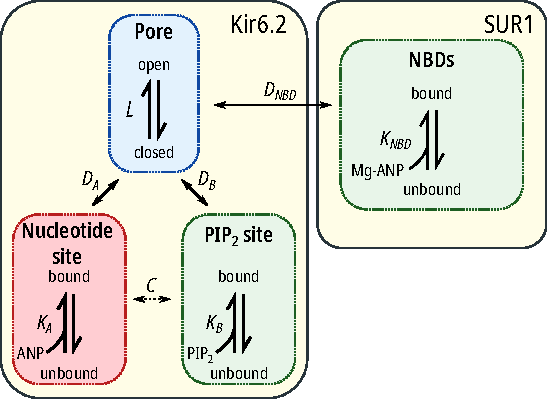
\includegraphics[width=0.7\textwidth]{regulation_diagram.pdf}
	\caption[Modes of regulation of K\ATP{}]{
	Adapted from \cite{puljung_cryo-electron_2018}.
	The open-closed equilibrium of the K\ATP{} channel pore (denoted as $L$) is energetically coupled to three different ligand binding sites.
	The four inhibitory nucleotide binding sites of Kir6.2 (labelled as NBS) bind either ATP or ADP (generalised to ANP) with an equilbrium binding constant $K_A$.
	The four stimulatory PIP\textsubscript{2} binding sites of Kir6.2 bind PIP\textsubscript{2} with an equilbrium binding constant $K_B$.
	The four stimulatory Mg-nucleotide binding site formed by the dimerisation of the NBDs of SUR1 (labelled as NBDs) bind either Mg-ATP or Mg-ADP (generalised to Mg-ANP) with an equilbrium binding constant $K_C$.
	Each binding domain interacts with the channel pore according to the factors $D_A$, $D_B$, and $D_{NBD}$ respectively.
	In addition, there is a potential coupling between the inhibitory nucleotide binding site of Kir6.2 and the stimulatory PIP\textsubscript{2} binding site of Kir6.2 described by the factor $C$.
	}\label{ch1fig:regulation_diagram}
\end{figure}

\subsection{Nucleotide regulation of the pancreatic K\ATP{} channel}

The physiological regulation of channel activity by nucleotides is the summed contribution of activation by Mg-nucleotides binding to the NBSs of SUR1, and inhibition by nucleotides binding to Kir6.2 \cite{nichols_adenosine_1996}.
To study these contributions experimentally, most research to date has relied on electrophysiological recordings of K\ATP{} currents.
Separating the contributions of the different classes of site has been achieved through a variety of methods.
Firstly, activation of the channel by Mg-nucleotides can be eliminated by removing Mg\textsuperscript{2+} ions from the solutions used to perfuse excised patches by inclusion of high concentrations of chelators such as EGTA \cite{gribble_mgatp_1998-1, proks_activation_2010-1}.
This experimental paradigm allows for the measurement of inhibition by nucleotides alone.
Secondly, activation of the channel by Mg-nucleotides can be isolated by introducing mutations which abolish nucleotide binding to Kir6.2 \cite{gribble_mgatp_1998-1, proks_activation_2010-1}.

Mutation of residues which are involved in nucleotide inhibition of the K\ATP{} channel can result in one of two functional effects.
In the first category are residues which, when substituted, reduce the sensitivity of the channel to nucleotide inhibition (i.e. increase the IC\textsubscript{50} for nucleotide inhibition) while not perturbing the intrinsic gating of the channel.
Mapping these residues to the the cryo-EM structures of ATP-bound K\ATP{} reveals that the residues in this category are invariably located close to the nucleotide binding site of Kir6.2.
The binding site is composed of part of the N-terminal region of one Kir6.2 subunit, and part of the C-terminal region of its neighbouring subunit.
Well characterised mutations of residues in this region of the N-terminus (R50 \cite{proks_involvement_1999, cukras_role_2002, john_molecular_2003, ribalet_molecular_2003, trapp_identification_2003, shimomura_mutations_2006}, G53 \cite{koster_dend_2008}) and C-terminus (I182 \cite{drain_katp_1998, koster_atp_2005, li_i182_2000}, K185 \cite{john_molecular_2003, ribalet_molecular_2003, trapp_identification_2003}, F333 \cite{tammaro_kir62_2005}, G334 \cite{drain_katp_1998, tammaro_kir62_2005, masia_atp-binding_2007-1, proks_activation_2010-1}) have no effects on single channel kinetics in the absence of nucleotide.
However, they are far less sensitive to inhibition by nucleotides.
The simplest hypothesis to explain this data given the location of the residues in the structures is that mutations of these residues perturb interactions between K\ATP{} and nucleotides, reducing the direct binding affinity of nucleotides for the inhibitory binding site (i.e. a reduction of $K_A$ in Figure \ref{ch1fig:regulation_diagram}).

Alternatively, mutations which do not affect intrinsic gating but reduce sensitivity to nucleotide inhibition may be affecting the relative selectivity of nucleotides for the closed state of the channel (i.e. $D_A$ approaches unity in Figure \ref{ch1fig:regulation_diagram}).
R201 was hypothesised to form part of the binding site as a cysteine \cite{proks_molecular_2004, antcliff_functional_2005} or histidine \cite{tammaro_functional_2006} substitution at this site results in reduced inhibition of K\ATP{} channels by nucleotides, without any changes in intrinsic gating .
Curiously, an alanine at this position results in K\ATP{} channels which exhibit both reduced sensitivity to ATP inhibition and reduced activation by PIP\textsubscript{2} \cite{shyng_structural_2000}.
Examining the cryo-EM structures suggests that this residue does not form direct contacts with bound ATP, and would therefore have to alter the nucleotide binding site allosterically - potentially by stabilising the short helix containing the critical F333 and G334 residues \cite{puljung_cryo-electron_2018}.
\citeauthor{ribalet_molecular_2003, john_molecular_2003} proposed that mutating R201 to an alanine instead acts by perturbing the preference of nucleotides for the closed state of the channel, increasing $D_A$.

The second category of residues are those which, when mutated, increase the $P_O$ of the channel and also affect the sensitivity of the channel to nucleotide inhibition.
This category is far larger, and these residues are found across both Kir6.2 and SUR1 structures.
Within the MWC framework in Figure \ref{ch1fig:regulation_diagram}, mutations which increase $L$ (and therefore increase the observed $P_O$) reduce the ability of nucleotides to inhibit the channel.
By increasing the stability of the open state, the selectivity of nucleotides for the closed state ($D_A < 1$) results in a decreased probability of nucleotide binding, and thus reducing inhibition.
Mutations within this category are difficult to fully characterise in the cell membrane environment due to the presence of phosphoinositides.
An observed increase in $P_O$ in an excised patch may either stem from an increase in $L$, or from an increase in $K_B$ or $D_B$.

Activation of K\ATP{} channels by Mg-nucleotides is not quite as trivial to measure in isolation.
The most common experimental paradigm used to isolate activatory effects is introducing a mutation into Kir6.2 which renders it insensitive to inhibition by nucleotides \cite{gribble_mgatp_1998-1, proks_activation_2010-1}.
Apllication of Mg-nucleotides to mutant channels such as Kir6.2-G334D then results in an increase in the burst duration and therefore the $P_O$ of K\ATP{} channels \cite{proks_activation_2010-1}.
This stimulatory effect is conferred by the NBSs of SUR1, as mutation of the Walker A motif in either NBS1 or NBS2 results in K\ATP{} channels which are no longer activated by Mg-nucleotides \cite{gribble_essential_1997,nichols_adenosine_1996}.

In ABC transporters, the conformational changes which allow substrate movement across the membrane are driven by ATP hydrolysis \cite{rees_abc_2009}.
In addition, there is strict coupling between ATP hydrolysis and channel gating in CFTR, an ABC family member which is in itself a chloride channel \cite{csanady_strict_2010-1}.
The NBDs of SUR1 are capable of hydrolysing ATP at rates comparable to that of CFTR \cite{matsuo_atp_1999, wet_studies_2007, puljung_cryo-electron_2018}.
\citeauthor{zingman_signaling_2001-1} used beryllium-fluoride and orthovanadate to stabilise the pre- and post-hydrolytic states of SUR1 respectively, and suggested that the post-hydrolytic state favoured channel opening.

However, \citeauthor{choi_testing_2008} analysed the microscopic reversibility of single-channel kinetics to determine whether ATP hydrolysis is coupled to channel gating.
Microscopic reversibility is a property of equilibrium systems such that their dynamics are time-reversible.
As ATP hydrolysis is irreversible and thus not in equilibrium, if channel gating is dependent on ATP hydrolysis it will not obey microscopic reversibility \cite{rothberg_testing_2001}.
Unlike for CFTR \cite{csanady_strict_2010-1}, \citeauthor{choi_testing_2008} found no evidence for ATP-dependent violations of microscopic reversibility in K\ATP{} channel gating, supporting the conclusion that ATP hydrolysis by the NBDs of SUR1 is not directly coupled to conformational changes of the channel.
In addition, Mg-ADP is sufficient to activate channel currents, obviating the need for ATP hydrolysis \cite{proks_activation_2010-1}.
It is most likely that the activatory function of Mg-nucleotides occurs in a similar manner as in inhibitory function of nucleotides; via an allosteric equilibrium effect on the channel pore ($D_{NBD}$ in Figure \ref{ch1fig:regulation_diagram}).

\subsection{PIP\textsubscript{2} regulation of the pancreatic K\ATP{} channel}

A conserved feature of Kir channels is that they are regulated by phosphoinositides, in particular PIP\textsubscript{2}, and Kir6.2 is no exception \cite{hibino_inwardly_2010, fan_anionic_1997, shyng_membrane_1998, baukrowitz_pip2_1998}.
Studying the nature of the regulation of K\ATP{} by PIP\textsubscript{2} is difficult experimentally due to the lack of control over PIP\textsubscript{2} concentrations, and our inability to precisely measure them.
Firstly, while the contaminating effects of intracellular nucleotides are removed by excision of a patch, the same is not true for PIP\textsubscript{2}.
The rundown of channel currents is largely attributable to dissociation and/or degradation of PIP\textsubscript{2} from the membrane patch, but rundown is a complex phenomenon and the relative amounts of PIP\textsubscript{2} in the membrane varies between patches and experimental conditions \cite{proks_running_2016-2}.
The hydrophobicity of PIP\textsubscript{2} means that perfusing a membrane patch results in accumulation of lipid in the membrane; it is impossible to reach an equilibrium with a known concentration.
An alternative is using analogs of PIP\textsubscript{2} with increased solubility due to shortening of the acyl chain length, such as dioctanoyl (diC\textsubscript{8}) PIP\textsubscript{2} \cite{rohacs_specificity_2003}.
While more soluble analogs are easier to work with and an experimenter can reach a quasi-equilibrium, we do not know how the concentration of diC\textsubscript{8} PIP\textsubscript{2} applied to a membrane equates to the concentration achieved in the membrane.
Another alternative is using polyamines such as neomycin as negative charge chelators; screening the negatively-charged phospholipid head groups present in the membrane away from their normal binding sites \cite{fan_anionic_1997, schulze_phosphatidylinositol_2003}.
This approach runs into the problems of both methods previously outlined; we do not know the precise correlation between the concentration of neomycin applied and the concentration of active, un-chelated PIP\textsubscript{2} in the membrane; and due to rundown it is impossible to reach a true equilibrium.

Despite all these complexities, there is still a great deal of research exploring how PIP\textsubscript{2} regulates K\ATP{} channel gating.
PIP\textsubscript{2} stimulates K\ATP{} channel currents by increasing channel open time and burst duration, and reduces the sensitivity of K\ATP{} channel currents to inhibition by nucleotides \cite{fan_phosphoinositides_1999, baukrowitz_pip2_1998, shyng_membrane_1998, fan_phosphoinositides_1999, enkvetchakul_kinetic_2000}.
The stimulatory effect occurs in the absence of SUR1, as the $P_O$ of Kir6.2\textgreek{D}C or Kir6.2-cGFP expressed alone is still enhanced by perfusion of PIP\textsubscript{2} \cite{fan_phosphoinositides_1999, enkvetchakul_kinetic_2000}.
However, the presence of SUR1 appears to enhance the ability of PIP\textsubscript{2} to stimulate channel currents \cite{baukrowitz_pip2_1998, shyng_membrane_1998, fan_phosphoinositides_1999, enkvetchakul_kinetic_2000}.
This enhancement has been proposed to occur through the interaction between the N-terminal of Kir6.2 and TMD0 of SUR1, and may account (at least in part) for the increase in 'intrinisc' $P_O$ observed when Kir6.2 and SUR1 are coexpressed \cite{pratt_n-terminal_2011}.
\citeauthor{pratt_n-terminal_2011} introduced a mutation (E128K) into the TMD0 region of SUR1 and found that K\ATP{} channels formed either with full-length mutant SUR1 or mutant TMD0 exhibited drastically reduced $P_O$ when compared to their wild-type counterparts.
In addition, the E128K mutation reduced the activation of channel currents by PIP\textsubscript{2}, and exposure to PIP\textsubscript{2} did not reduce the sensitivity of E128K channels to nucleotide inhibition.
These findings highlight the complexity of the regulatory role of SUR1, and also the difficulty in separating effects on intrinsic channel gating from effects on PIP\textsubscript{2} regulation, given the difficulty in measuring and controlling the latter.

The second functional aspect of PIP\textsubscript{2} modulation is its effects on sensitivity of K\ATP{} channels to nucleotide inhibition.
Application of PIP\textsubscript{2} reduces the ability of nucleotides to inhibit K\ATP{} channels, and reduction of PIP\textsubscript{2} activity from rundown or application of neomycin increases the ability of nucleotides to inhibit K\ATP{} channels \cite{baukrowitz_pip2_1998, shyng_membrane_1998, fan_phosphoinositides_1999, enkvetchakul_kinetic_2000}.
In addition, photoaffinity labelling of Kir6.2 by ATP analogs is reduced in the presence of phosphoinositides \cite{wang_compromised_2002}.
This phenomenon can be explained by the allosteric effects of increasing channel $P_O$, which would result in a corresponding decrease in nucleotide binding and inhibition due to the energetic coupling of the nucleotide binding site and the channel pore ($D_A$ in Figure \ref{ch1fig:regulation_diagram}) \cite{proks_modeling_2009}.
However, it has also been hypothesised that there is an additional interaction between nucleotides and PIP\textsubscript{2} which is not mediated through energetic coupling to the channel pore ($C$ in Figure \ref{ch1fig:regulation_diagram}) \cite{fan_phosphoinositides_1999, proks_modeling_2009, haider_identification_2007}.
This interaction could be due to direct competition between PIP\textsubscript{2} and nucleotides for the same site, or by local allosteric interactions which energetically disfavour binding of one ligand when the other is already bound.

While the cryo-EM structures of K\ATP{} were not able to capture a PIP\textsubscript{2}-bound state, there is a crystal structure of Kir2.2 complexed with PIP\textsubscript{2} which suggests that the Kir6.2 PIP\textsubscript{2} binding site is not the same as the nucleotide binding site \cite{hansen_structural_2011}.
This is supported by mutagenic electrophysiological studies, which show that substitutions at residues which alter nucleotide sensitivity but not $P_O$ also do not affect activation of channel currents by PIP\textsubscript{2} (with the notable exception of R201, which is discussed previously) \cite{fan_anionic_1997, shyng_structural_2000, schulze_phosphatidylinositol_2003, haider_identification_2007}.
This does not rule out the possibility of separate but overlapping sites for nucleotide and PIP\textsubscript{2} binding, and whether nucleotides and PIP\textsubscript{2} are able to simultaneously bind to the same subunit remains an open question \cite{enkvetchakul_gating_2003-2, proks_modeling_2009}.

\section{Fluorescence methods in ion channel research}

\subsection{Fluorescence as a tool}

\subsection{Forster resonance energy transfer}

\subsection{Unnatural amino acid incorporation}

\chapter{\label{ch:2-methods}Methods}

\graphicspath{{figures/ch2/}}

\minitoc 

\section{Molecular biology.}
Human Kir6.2 and SUR1 were subcloned into pcDNA4/TO and pCGFP\_EU vectors for expression of wild-type and GFP-tagged constructs, respectively.
pcDNA4/TO and pANAP were obtained from Addgene.
peRF1-E55D and pCGFP\_EU were kind gifts from the Chin Laboratory (MRC Laboratory of Molecular Biology, Cambridge, UK) and the Gouaux Laboratory (Vollum Institute, Oregon, USA) respectively.
Amber stop codons and point mutations were introduced using the QuikChange XL system (Stratagene; San Diego, CA).
All constructs were confirmed by DNA sequencing (DNA Sequencing and Services, University of Dundee, Scotland).

\section{Cell culture and channel expression}
HEK-293T cells were obtained from and verified/tested for mycoplasma by LGC standards (ATTC CRL-3216, Middlesex, UK).
Our working stock tested negative for mycoplasma contamination using the MycoAlert Mycoplasma Detection Kit (Lonza Bioscience; Burton on Trent, UK).
Cells were plated onto either poly-L-lysine coated borosilicate glass coverslips (VWR International; Radnor, PA) or poly-D-lysine coated glass-bottomed FluoroDishes (FD35-PDL-100, World Precision Instruments).
ANAP-tagged Kir6.2 constructs were labelled using amber stop codon suppression as described by Chatterjee et al.
Transfections were carried out 24 hours after plating using TransIT-LT1 (Mirus Bio LLC; Madison, WI) at a ratio of 3 \si{\micro\litre} per \si{\micro\gram} of DNA.
Unless specified otherwise, all transfections included a Kir6.2 construct with an amber stop codon (TAG) at position 311 (Kir6.2-W311\textsuperscript{TAG}), SUR1, pANAP and eRF1-E55D in the ratio 0.5:1.5:1:1.
Transfected cells cultured in Dulbecco’s Modified Eagle Medium (Sigma; St. Louis, MO) + 10\% foetal bovine serum, \SI{100}{\Unit\per\milli\litre} penicillin and \SI{100}{\micro\gram\per\milli\litre} streptomycin (Thermo Fisher Scientific; Waltham, MA) supplemented with \SI{20}{\milli\Molar} ANAP (free acid, AsisChem; Waltham, MA).
Cells were incubated at \SI{33}{\degreeCelsius} and in the presence of \SI{300}{\micro\Molar} tolbutamide to enhance protein expression and channel trafficking to the plasma membrane.
eRF1-E55D was included to increase efficiency of ANAP incorporation.
Experiments were carried out 2-4 days after transfection.
We also expressed constructs labelled with ANAP at positions I182, F183, F198, and I210.
Kir6.2-F183*, Kir6.2-F198*, and Kir6.2-I210* co-expressed with SUR1 did not produce sufficient currents for subsequent experimentation.
Mutations at I182 are known to produce profound effects on nucleotide inhibition of K\textsubscript{ATP}.
Thus, we did not consider this site for further experimentation.

\section{Western blots}
Transfected HEK-293T cells grown in 6-well plates were harvested in cold PBS (Life Technologies Limited; Paisley, UK), pelleted at 0.2 x g for 2.5 minutes and resuspended in lysis buffer containing 0.5\% Triton X-100, \SI{100}{\milli\Molar} potassium acetate, and a cOmplete protease inhibitor tablet (1 tablet/\SI{50}{\milli\litre}, Roche; Basel, Switzerland), buffered to pH 7.4.
After a 30-minute benzonase (Sigma) treatment at room temperature, samples were mixed with a DTT containing reducing agent and loading buffer (NuPAGE, Invitrogen; Carlsbad, CA) and run on a precast Bis-Tris 4-12\% poly-acrylamide gel at \SI{200}{\volt} for 40 minutes.
Proteins were wet transferred overnight onto polyvinylidene difluoride (PVDF) membranes (Immobilon P, Merck Millipore; Burlington, VT) in \SI{25}{\milli\Molar} Tris, \SI{192}{\milli\Molar} glycine, 20\% methanol, and 0.1\% SDS at \SI{10}{\volt} on ice.
Membranes were blocked with 5\% milk in TBS-Tw (\SI{150}{\milli\Molar} NaCl, 0.05\% Tween 20, \SI{25}{\milli\Molar} Tris, pH 7.2) before staining for 30 minutes with a 1:1000 dilution of rat anti-HA monoclonal antibody in TBS-Tw (clone 3F10, Roche).
After washing with TBS-Tw, membranes were incubated for 30 minutes with a 1:20,000 dilution of HRP-conjugated goat anti-rat polyclonal antibodies in TBS-Tw (Jackson ImmunoResearch; Ely, UK).
Detection was performed using the SuperSignal West Pico Chemiluminescent Substrate (Thermo Fisher) and a C-DiGit Blot Scanner (Licor Biosciences; Lincoln, NE).
Analysis was performed using custom code written in Python.

To confirm our ability to express full-length Kir6.2*-GFP, we performed western blots for HA-tagged Kir6.2 constructs in detergent-solubilized HEK-293T cells (Figure 1—Figure supplement 1C).
The HA tag plus a short linker (YAYMEKGITDLAYPYDVPDY) was inserted in the extracellular region following helix M1 of Kir6.2 between L100 and A101.
Transfection of wild-type Kir6.2-HA or Kir6.2-HA-GFP resulted in two bands on the western blots.
The upper bands were close to the expected sizes for full-length Kir6.2-HA and Kir6.2-HA-GFP (\SI{46}{\kilo\dalton} and \SI{77}{\kilo\dalton}, respectively).

We consistently observed a lower molecular weight band as well.
This band must correspond to an N-terminally truncated Kir6.2 product, as the apparent molecular weight shifted with addition of the C-terminal GFP tag.
Based on the molecular weight, we predict that the truncated protein product initiated from a start codon in the first transmembrane domain.
Therefore, we believe it is unlikely that this protein would form functional channels or traffic to the plasma membrane.
When Kir6.2-W311\textsuperscript{TAG}-HA or Kir6.2-W311\textsuperscript{TAG}-HA-GFP were co-transfected with SUR1, pANAP, and eRF1-E55D, and cells were cultured in the presence of ANAP, the western blots were similar to wild-type Kir6.2-HA or Kir6.2-HA-GFP.
Over 90\% full-length Kir6.2*-HA-GFP was produced under these conditions (Figure 1—Figure supplement 1D).
We were unable to quantify the percentage of full-length Kir6.2*-HA produced as the C-terminally truncated band resulting from termination at the TAG codon was very similar in size to the N-terminally truncated band.
Co-expression with SUR1 increased the percentage of full-length Kir6.2*-HA-GFP produced (Figure 1—Figure supplement 1D).
In the absence of ANAP, we did not observe any full-length Kir6.2, indicating that there was no read-through of the amber (TAG) stop codon (Figure 1—Figure supplement 1D).

\section{Confocal microscopy}
Confocal imaging was performed using a spinning-disk system (Ultra-VIEW VoX, PerkinElmer; Waltham, MA) mounted on an IX81 microscope (Olympus; Southend-on-Sea, UK) with a Plan Apo 60x oil immersion objective (NA = 1.4), provided by the Micron Advanced Bioimaging Unit, Oxford.
Transfected HEK-293T cells were incubated for 15 minutes with \SI{1}{\nano\Molar} CellMask Deep Red (Thermo Fisher) to stain plasma membranes before washing with PBS and imaging.
ANAP was excited with a solid-state laser at \SI{405}{\nano\Molar}.
GFP and CellMask were excited with an argon laser at \SI{488}{\nano\Molar} and \SI{633}{\nano\Molar} respectively.
Images were captured on an EMCCD camera (ImagEM; Hamamatsu Photonics; Welwyn Garden City, UK) binned at 2 x 2 pixels and analysed using Python.
A median filter with a box size of 32 x 32 pixels was applied to improve the signal-to-noise ratio by reducing background fluorescence.

We examined the surface expression of our ANAP-labelled constructs using confocal microscopy (Figure 1—Figure supplement 1A,B).
When Kir6.2-W311\textsuperscript{TAG}-GFP was co-transfected with SUR1 along with pANAP and eRF1-E55D in the presence of ANAP, the ANAP and GFP fluorescence were co-localized at the plasma membrane.
When wild-type Kir6.2-GFP was transfected under the same conditions, only GFP fluorescence was observed at the plasma membrane.
ANAP fluorescence was diffuse and confined to the cytoplasm or intracellular structures.
Thus, the plasma-membrane ANAP signal was specific for Kir6.2*-GFP.

\section{Surface expression assays}
We measured surface expression of HA-tagged Kir6.2 subunits using an approach outlined by Zerangue et al.
Cells were plated on \SI{19}{\milli\metre} coverslips coated with poly-L-lysine and transfected as described above.
Following incubation, cells were rinsed with PBS before fixation with 10\% formalin for 30 minutes at room temperature.
After washing again, cells were blocked with 1\% BSA in PBS for 30 minutes at \SI{4}{\degreeCelsius} before a 1-hour incubation at \SI{4}{\degreeCelsius} with a 1:1000 dilution (in PBS) of rat anti-HA monoclonal antibodies.
Cells were then washed 5 times on ice with 1\% BSA in PBS followed by a 30-minute incubation at \SI{4}{\degreeCelsius} with a 1:2000 dilution of HRP-conjugated goat anti-rat polyclonal antibodies.
Cells were washed 5 times in PBS + 1\% BSA and 4 times in PBS.
Coverslips were removed from the culture dishes and placed in clean, untreated dishes for measurement.
\SI{300}{\micro\litre} of SuperSignal ELISA Femto Maximum Sensitivity Substrate (Thermo Fisher) was added to each sample and the luminescence was measured using a Glomax 20/20 Luminometer (Promega; Madison, WI) after a 10 second incubation.

HEK-293T cells were transfected with Kir6.2 constructs with or without a TAG stop codon corresponding to position 311.
Cells were co-transfected with pANAP and eRF1-E55D in the presence or absence of SUR1 and cultured with or without ANAP.
Wild-type Kir6.2-HA and Kir6.2-HA-GFP in the presence of SUR1 were included as positive controls.
Kir6.2 constructs with no HA tag served as negative controls.
In the presence of ANAP, we observed strong trafficking of Kir6.2*-HA-GFP to the plasma membrane, but much less trafficking of Kir6.2*-HA (Figure 1—Figure supplement 1E).
When cells were cultured in the absence of ANAP, we observed little to no Kir6.2 surface expression from cells that were transfected with Kir6.2-W311\textsuperscript{TAG}-HA or Kir6.2-W311\textsuperscript{TAG}-HA-GFP, suggesting that prematurely truncated constructs did not traffic to the plasma membrane.
In the absence of SUR1, surface expression was weak for both wild-type and tagged constructs, despite the reported ability of Kir6.2-GFP to traffic to the plasma membrane in the absence of SUR1.

\section{Epifluorescence imaging and spectroscopy}
Epifluorescence imaging and spectroscopy were performed using a Nikon Eclipse TE2000-U microscope with a 60x water immersion objective (Plan Apo VC, NA = 1.2, Nikon; Kingston upon Thames, UK) or a 100x oil immersion objective (Nikon, Apo TIRF, NA = 1.49).
Imaging of ANAP was performed using a \SI{385}{\nano\metre} LED source (ThorLabs; Newton, NJ) with a \SI{390/18}{\nano\metre} band-pass excitation filter, an MD416 dichroic and a \SI{479/40}{\nano\metre} band-pass emission filter (all from ThorLabs).
GFP was imaged using a \SI{490}{\nano\metre} LED source (ThorLabs) with a \SI{480/40}{\nano\metre} band-pass excitation filter, a DM505 dichroic, and a \SI{510}{\nano\metre} long-pass emission filter (all from Chroma; Bellows Falls, VT).
Fluorescence spectra were collected by exciting ANAP as above but using a \SI{400}{\nano\metre} long-pass emission filter (ThorLabs), then passing emitted light through an IsoPlane 160 Spectrometer (Princeton Instruments; Trenton, NJ) with a \SI{300}{\gram\per\milli\metre} grating.
Images were collected with \SI{1}{\second} exposures on a Pixis 400BR\_eXcelon CCD (Princeton Instruments).

\section{Electrophysiology.}
Patch pipettes were pulled from thick-walled borosilicate glass capillaries (GC150F-15, Harvard Apparatus; Holliston, MA) to a resistance of \SIrange{1.5}{2.5}{\mega\ohm} when filled with pipette solution.
Currents were recorded at \SI{-60}{\milli\volt} from excised inside-out patches using an Axopatch 200B amplifier equipped with a Digidata 1322A digitizer and using pClamp 10 software (Molecular Devices; San Jose, CA).
Currents were low-pass filtered at \SI{5}{\kilo\hertz} and digitized at \SI{20}{\kilo\hertz}.
The bath solution (intracellular) contained \SI{140}{\milli\Molar} KCl, \SI{10}{\milli\Molar} HEPES, \SI{1}{\milli\Molar} EDTA and \SI{1}{\milli\Molar} EGTA (pH 7.3 with KOH).
The pipette solution (extracellular) contained \SI{140}{\milli\Molar} KCl, \SI{10}{\milli\Molar} HEPES and \SI{1}{\milli\Molar} EDTA (pH 7.4 with KOH).
All experiments were carried out in Mg\textsuperscript{2+}-free conditions.
Currents were leak corrected using the current remaining in bath solution containing \SI{5}{\milli\Molar} barium acetate at \SI{+60}{\milli\volt}, assuming a linear leak with a reversal potential of \SI{0}{\milli\volt}.
Inhibition was calculated and corrected for rundown by alternating test concentrations of nucleotide solution with nucleotide-free solution, then expressing the test currents as a fraction of the average of the control currents before and after the test solution as described previously.

\section{FRET calculations}
We calculated the expected FRET efficiency between ANAP incorporated at amino acid position 311 and a docked TNP-ATP molecule as described previously.
The equivalency between FRET efficiency (measured as ANAP quenching) and nucleotide binding is based on two main assumptions.
Firstly, we assume that the observed quenching from a bound nucleotide does not differ dramatically between open and closed states of the channel.
As there is no open-state structure of K\textsubscript{ATP}, we do not know exactly how much relative movement would occur between a bound TNP-ATP and Kir6.2-W311.
However, based on cryo-EM structures of apo and nucleotide-bound Kir6.2 we do not expect to see a change in the distance between these two positions.

Secondly, we assume that the ANAP and TNP-ATP molecules on each subunit do not undergo energy transfer with those on other subunits to an extent which would dramatically change the observed quenching.
At saturating TNP-ATP concentrations, where each ANAP-labelled site on Kir6.2 is occupied, FRET between ANAP and the closest acceptor will be kinetically favoured and the overall FRET efficiency will not be affected by cross-talk between neighbouring sites.
In the limiting case, at low TNP-ATP concentrations, one would expect a large proportion of Kir6.2 tetramers (with four ANAP-labelled binding sites) bound to only a single TNP-ATP molecule.
In this case, we expect a 4\% overestimation of nucleotide binding as calculated using a numerical method to simulate a single TNP-ATP acceptor with multiple ANAP donors based on the distances calculated from our docking.
This may have resulted in our binding curves becoming artifically shallow at low concentrations.
However, this difference is not significant in the context of our measurements as it is smaller than the observed error of our measurements at low TNP-ATP concentrations.

\section{Unroofed binding measurements.}
Unroofed membranes were prepared as described previously.
A coverslip plated with transfected HEK-293T cells was removed from the culture media and rinsed with PBS.
The coverslip was then briefly sonicated using a probe sonicator (Vibra-cell; Newtown, CT) leaving behind adherent plasma membrane fragments.
Cells cultured on FluoroDishes were rinsed and sonicated directly in the dish.
Unroofed membrane fragments were nearly invisible in bright-field images and identified by their GFP and ANAP fluorescence.
Fluorescent TNP-nucleotides (Jena Bioscience; Jena, Germany) were diluted in bath solution and perfused onto unroofed membranes using a valve controlled microvolume superfusion system (\si{\micro}Flow, ALA Scientific Instruments; Farmingdale, NY).

Fluorescence spectra were collected as described above.
A region of interest corresponding to the membrane fragment was manually selected and line-averaged for each wavelength.
A similarly sized region of background was selected and averaged, then subtracted from the spectrum of interest.
After subtraction, ANAP intensity was calculated by averaging the fluorescence intensity measured between \SI{469.5}{\nano\metre} and \SI{474.5}{\nano\metre}.
Bleaching was corrected by fitting the normalised ANAP intensity of exposures taken during perfusion with nucleotide-free solution to a single exponential decay of the form
\begin{equation} \label{eq:bleaching}
    \frac{F}{F_{max}} = ae^{kt} + (1 - a)
\end{equation}
then using the fit to correct the intensity of exposures taken during perfusion with test nucleotide solutions.

Some experiments were excluded from further analysis due to obvious cross-contamination between different solutions within the \si{\micro}Flow superfusion system.
These were identified by noticeable colour changes in the solution in the delivery tubes.

\section{Patch-clamp fluorometry.}
The tip of the patch pipette was centred on the slit of the spectrometer immediately after patch excision.
Currents were measured as described above.
Fluorescence emission spectra from the excised patch were acquired concurrently with current measurements, both during test solution application as well as nucleotide-free solution.
Background subtraction was slightly imperfect due to the exclusion of TNP-ATP from volume of the glass of the pipette, resulting in spectra that have negative intensities at the TNP-ATP peak at high nucleotide concentrations.
However, this over-subtraction does not affect the size of the ANAP peak, which we used to quantify nucleotide binding.

ANAP bleaching was corrected as for the unroofed binding experiments with Equation \ref{eq:bleaching} (Figure 2-Figure supplement 3A).
Due to the lower signal-to-noise ratio for PCF compared to the unroofed membranes, we performed experiments from both high-to-low and low-to-high TNP-ATP concentrations to minimise artifacts from our bleaching corrections.
Kir6.2*-GFP + SUR1 showed consistent bleaching time courses (Figure 2-Figure supplement 3B) and an average of 34\% of the initial ANAP fluorescence intensity remained at the end of each experiment (Figure 2-Figure supplement 3C).

Some experiments were excluded from further analysis due to low fluorescence intensity, as we were concerned about a low signal to noise ratio influencing our results.

\section{Data processing and presentation.}
Raw spectrographic images and current traces were pre-processed in Python and Clampfit (Axon) before analysis with R.
Where applicable, all experimental data points are displayed in each figure.
The number of experiments is reported in the figure legends and tables.
To help visualise uncertainty and prevent some data points being hidden, they are arranged with a small amount of horizontal jitter; vertical position remains unaffected.
Unless otherwise stated, summary statistics are overlaid as the mean with error bars representing the standard error of the mean.
Where these error bars are not visible, they are smaller than the size of the point used for the mean.

Hill fits to fluorescence quenching were nonlinear least-squares fits to the following equation:
\begin{equation} \label{eq:hill}
    \frac{y}{y_{max}} = 1 - E_{max} + \frac{E_{max}}{1 + 10^{(EC_{50} - [TNPATP]) \cdot h}}
\end{equation}
where $y$ represents normalised fluorescence intensity and $EC_{50}$ and $[TNPATP]$ are $\log_{10}$ values.
Current inhibition data were fit to the same equation but with $y$ representing normalised current magnitude, $IC_{50}$ instead of $EC_{50}$, and $I_{max}$ instead of $E_{max}$.

\section{Computational docking.}
Computational docking of TNP-ATP into the nucleotide binding site of Kir6.2 was performed using AutoDock-Vina and Pymol (Schrödinger, LLC; New York, NY).
11 TNP-ATP structures from the Protein Data Bank (PDB accession \#s 1I5D, 3AR7, 5NCQ, 5SVQ, 5XW6, 2GVD, 5A3S, 2PMK, and 3B5J) were used as starting poses and a 15x11.25x15 \si{\angstrom} box was centred on the ATP bound to Kir6.2 in PDB accession \#6BAA.
Protonation states for each residue were assigned using PDB2PQR and PROPKA 3.0.
The modal highest-scoring pose from the docking run was selected (PDB accession \#5XW6) and distances were measured from a pseudo atom at the centre of the fluorescent moiety.
TNP-ATP (PDB \#3AR7) was positioned into the first nucleotide binding domain of SUR1 (PDB \#6PZI) using the alignment tool in Pymol.

\section{Chemicals and stock solutions.}
Unless otherwise noted, all chemicals were obtained from Sigma.
TNP-ATP was obtained as a \SI{10}{\milli\Molar} aqueous stock from Jena Bioscience and stored at \SI{-20}{\degreeCelsius}. \SI{1}{\milli\Molar} aqueous stocks of ANAP-TFA were prepared by dissolving the free acid in \SI{30}{\milli\Molar} NaOH, and were stored at \SI{-20}{\degreeCelsius}. Tolbutamide stocks (\SI{50}{\milli\Molar}) were prepared in \SI{100}{\milli\Molar} KOH and stored at \SI{-20}{\degreeCelsius}.

\chapter{\label{ch:3}Measuring nucleotide binding to K\ATP} 

\graphicspath{{figures/ch3/}}

\minitoc

\section{Designing a nucleotide binding assay}

\subsection{Criteria for a useful assay for nucleotide binding to Kir6.2}

Previous approaches to measuring nucleotide binding directly to the different binding sites  of K\ATP{} have relied on isolating binding to individual classes of site by disrupting protein function; either by introducing mutations which abolish binding to a particular site, by measuring binding to Kir6.2 or SUR1 alone, or by measuring binding to fragments of the two subunits.

Two key studies have attempted to measure nucleotide binding to the inhibitory site on Kir6.2 directly.
The first relied on photoaffinity labelling of Kir6.2 by the radionucleotide 8-azido-[\textgreek{g}-\textsuperscript{32}P]-ATP \cite{tanabe_direct_1999}.
In these experiments, Kir6.2 with an N-terminal FLAG-tag was expressed in COS-7 cells, and membranes were separated by centrifugation.
After incubating the membrane fractions with 8-azido-[\textgreek{g}-\textsuperscript{32}P]-ATP, application of UV light results in a covalent linkage between the bound 8-azido-[\textgreek{g}-\textsuperscript{32}P]-ATP and Kir6.2.
After separation of the membrane fraction proteins on a gel, the quantity of bound radionucleotide can then by quantified by counting the radioactivity of the band corresponding to Kir6.2.
These experiments were able to definitively establish that the inhibitory nucleotide binding site of K\ATP{} was on Kir6.2, and suggested that the Kir6.2 binding site possessed a lower affinity toward the radionucleotide than the SUR1 binding sites.

The second made use of a fluorescent congener for ATP, trinitrophenyl (TNP)-ATP.
TNP-ATP had previously been used in binding measurements of purified proteins due to it's increased quantum yield (and thus increase in observed fluorescence) upon binding (need a ref).
TNP-ATP is most commonly used as an antogonist of P2X receptors, which are also sensitive to endogenous ATP.
The authors measured binding of TNP-ATP to the purified carboxyl terminal of Kir6.2 (residues 169 to 354) solubilised by linking it to mannose binding protein (MBP) \cite{vanoye_carboxyl_2002}.
The increased fluoresence of TNP-ATP when bound to the Kir6.2-MBP construct could be measured in a spectrometer, and allowed for equlibrium measurements of nucleotide binding.
These experiments were able to establish an initial estimate for the binding affinity of the Kir6.2 site for TNP-ATP at \SI{5}{\micro\Molar}.
These findings were replicated in a similar study, which used fusion proteins constructed from residues 170 to 390 of Kir6.2 fused to glutathione-S-transferase (GST) and estimated a binding affinity of \SI{5}{\micro\Molar} \cite{wang_inhibition_2006}.

These studies were hampered by the need to isolate the Kir6.2 binding site from the two SUR1 binding sites, which leads to unphysiological experimental conditions.
To improve on these methods, an ideal assay measuring nucleotide binding to the K\ATP{} channel neeeds to fulfill a number of criteria.

\begin{enumerate}
	\item We need sufficient spatial sensitivity to distinguish between different classes of binding site; i.e. the assay should be capable of distingushing binding to Kir6.2 from binding to NBS1 or NBS2.
	\item We should be able to measure binding to a channel which we know is functional, so our experimental conditions cannot be drastically different from those used to measure channel function.
	\item There should be minimal perturbation of the channel in order for binding measurements to be physiologically relevant.
	\item For accurate measures of affinity, binding should be at equilibrium so we cannot use covalent interactions or other forms of non-equilibrium labelling.
	\item We should be able to achieve a higher temporal resolution.
\end{enumerate}

TO fulfill these criteria, we used an approach involving a fluorescent unnatural amino acid, ANAP.
ANAP has been used increasing widely in the study of ion channel structure and function due to several desirable qualities.

\begin{enumerate}
	\item It is smaller than traditional fluorescent labels such as fluorescent proteins or rhodamine derivatives.
	Therefore, it should be less perturbing to the function of the protein it labels.
	\item As it is an amino acid, it can be site-specifically inserted into any protein.
	This avoids the issues of other small chemical dyes which are targeted to a site via post-translational covalent modifications, typically by reacting with a cysteine residue.
	While this can be avoided in some proteins by mutating each cysteine residue to an alternative residue to avoid off-target labelling, there are functionally important cysteines in the K\ATP{} channel which cannot be mutated.
	In addition, this does not solve the problem of off-target labelling of other membrane proteins
	\item ANAP is environmentally sensitive, which has been used to great effect in other studies.
	Notably, the peak emission ranges from \textasciitilde450nm to \textasciitilde490nm depending on the hydrophobicity of the surrounding environment.
\end{enumerate}

Initially, we hoped that the environmental sensitivity of ANAP fluorescence might be sufficient for the peak fluorescence of an ANAP residue inserted into an ATP binding site to measureably change when ATP was bound.
Unfortunately, when we introduced ANAP directly into the Kir6.2 binding site in place of residues I182 or F183 we were not able to observe any functional K\ATP{} channels at the cell membrane.

Instead, we turned to FRET as a reporter for ATP binding.
As ATP itself is not fluorescent, and has no intrinsic fluorescence quenching, we turned to TNP-ATP (Figure \ref{ch3fig:chemical_structures}).
TNP-ATP is an excellent FRET partner of ANAP, as evidenced by the good overlap in the TNP emission spectra and the ANAP extinction spectra (Figure \ref{ch3fig:spectral_overlap}).
This leads to a theoretical distance-dependency of FRET which is most sensitive between \SIrange{20}{60}{\angstrom} (Figure \ref{ch3fig:fret_efficiency}) with a calculated R0 of \SI{38.4}{\angstrom}.

\begin{figure}[h]
	\centering
	\begin{subfigure}[t]{0.4\textwidth}
		\caption{}\label{ch3fig:chemical_structures}
		\centering
		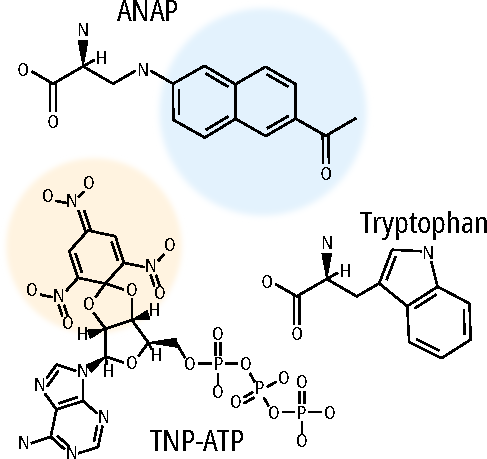
\includegraphics[width=\textwidth]{chemical_structures.pdf}
	\end{subfigure}
	\hfill
	\parbox[t]{0.5\textwidth}{
	\begin{subfigure}[t]{0.5\textwidth}
		\caption{}\label{ch3fig:spectral_overlap}
		\centering
		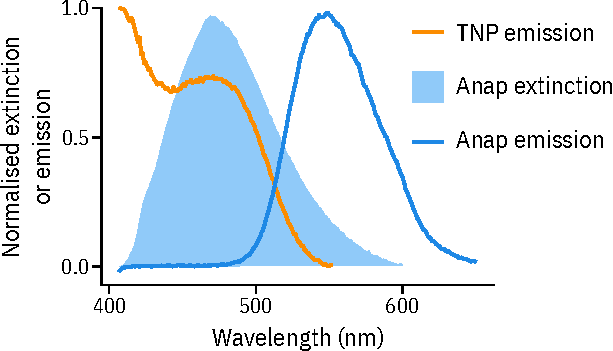
\includegraphics[width=\textwidth]{spectral_overlap.pdf}
	\end{subfigure}
	\hfill
	\begin{subfigure}[t]{0.5\textwidth}
		\caption{}\label{ch3fig:fret_efficiency}
		\centering
		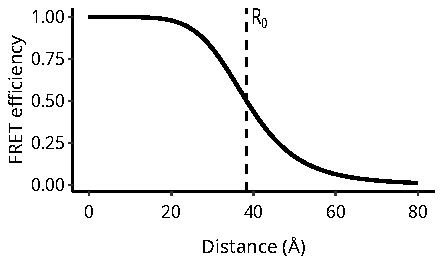
\includegraphics[width=\textwidth]{fret_efficiency.pdf}
	\end{subfigure}
	}
	\caption[ANAP and TNP-nucleotides as FRET pairs]{
		\subref{ch3fig:chemical_structures} Chemical structures of ANAP and TNP-ATP shown with the fluorescent moieties highlighted in blue (ANAP) or orange (TNP-ATP).
		\subref{ch3fig:spectral_overlap} Normalised emission spectra (solid lines) of ANAP (blue) and TNP-nucleotides (orange) overlayed on the normalised extinction spectra of ANAP (filled light blue area).
		Extinction spectra were measured from ANAP and TNP-nucleotides separately in aqueous solution.
		ANAP emission is the averaged spectra from W311*+SUR1 expressed in unroofed membranes.
		\subref{ch3fig:fret_efficiency} Theoretical FRET efficiency displayed as a function of the distance between donor and acceptor fluorophores.
		The curve was calculated as a function of the overlap shown in \subref{ch3fig:spectral_overlap}.
		The full formula is discussed in Chapter \ref{ch:2-methods}.
	}

\end{figure}

\subsection{Choosing a site to incorporate ANAP}

THe theoretical R0 of \SI{38.4}{\angstrom} for FRET between ANAP and TNP-ATP allowed for flexibility when choosing a site to incorporate ANAP.
Ideally, a residue should be chosen to maximise the following aims:

\begin{enumerate}
	\item The incorporated ANAP needs to be close enough to the nucleotide binding site of interest to report a quantifiable change in FRET when TNP-ATP is bound.
	This would not have to be close enough for \SI{100}{\percent} FRET to occur, but the greater the efficiency achieved the higher the signal-to-noise ratio would be for measuring binding.
	\item It also needs to be far enough from each other class of nucleotide binding site to avoid quenching by TNP-ATP bound to other sites.
	\item In addition to avoiding interference from other classes of binding site, we also need to avoid cross-talk between nucleotide binding sites of the same class on different subunits, as this would lead to difficulty interpreting the measured quenching.
	The ideal theoretical solution would be labelling only one nucleotide binding site per ion channel, but without using a concatemer this is not so easy in practise.
	\item More practically, incorporation of ANAP should not lead to drastic changes in nucleotide binding or channel gating properties, and the complete K\ATP{} channel needs to be expressed on the membrane.
\end{enumerate}

To narrow down which residues could be candidates for ANAP incorporation to measure binding at Kir6.2, we took three cryo-EM structures of K\ATP{} with ATP bound and computationally docked TNP-ATP into the nucleotide binding pocket (Figure \ref{ch3fig:docking}).
To assess the validity of computationally docking a ligand to each structure, we first attempted to dock ATP into the inhibitory binding pocket of Kir6.2 to check that the highest-scoring binding poses were similar to those observed in the cryo-EM structures.
Docking ATP to both \#6C3P and \#6C3O yielded binding poses which were very similar to the pose found in the cryo-EM structures (Figures \ref{ch3fig:6c3p_docking}, \ref{ch3fig:6c3o_docking}).
However, docking ATP to \#6BAA resulted in binding poses which were in a flipped orientation relative to the pose found in the cryo-EM structure (Figure \ref{ch3fig:6baa_docking}).

We then took TNP-nucleotide structures from eleven different X-ray diffraction and cryo-EM structures published on RCSB to dock to the Kir6.2 binding site of K\ATP{}.
For both \#6BAA and \#6C3P we observed that the three highest scoring binding poses for TNP-nucleotides closely resemble those of the ATP solved in complex with the channel (Figures \ref{ch3fig:6baa_docking}, \ref{ch3fig:6c3p_docking}).
It is not so clear for \#6C3O, for which the highest scoring poses are not in agreement with each other or the solved structure of ATP.

Based on the predicted TNP-ATP poses for \#6BAA and \#6C3P, we could narrow down potential ANAP incorporation sites to within \SI{25}{\angstrom} of the centre of the TNP-moiety, at which distance we would expect to see over \SI{90}{\percent} FRET efficiency when TNP-ATP is bound to Kir6.2.
In addition, we excluded residues which fell within \SI{45}{\angstrom} of NBS1 or NBS2, as this restricts the potential FRET between TNP-ATP bound at these sites and our chosen residue to roughly \SI{25}{\percent} or less.
While we can exclude residues which fall too close to the NBS's of SUR1, the close proximity of the Kir6.2 nucleotide binding sites to each other means that we cannot exclude intersubunit FRET occuring; i.e. TNP-ATP binding to a neighbouring subunit will also be able to quench ANAP to a certain extent. However, this occurs in a predictable way that we can measure and account for.

We ended up with one residue which fulfilled these criteria and for which membrane expression of the ANAP-incorporated channel could be detected: W311.
It is a bulky hydrophobic residue similar to ANAP, and no mutations at this residue have been previously identified to alter K\ATP{} function.

\begin{figure}[h]
	\centering
	\begin{subfigure}[t]{0.30\textwidth}
		\caption{}\label{ch3fig:6baa_docking}
		\centering
		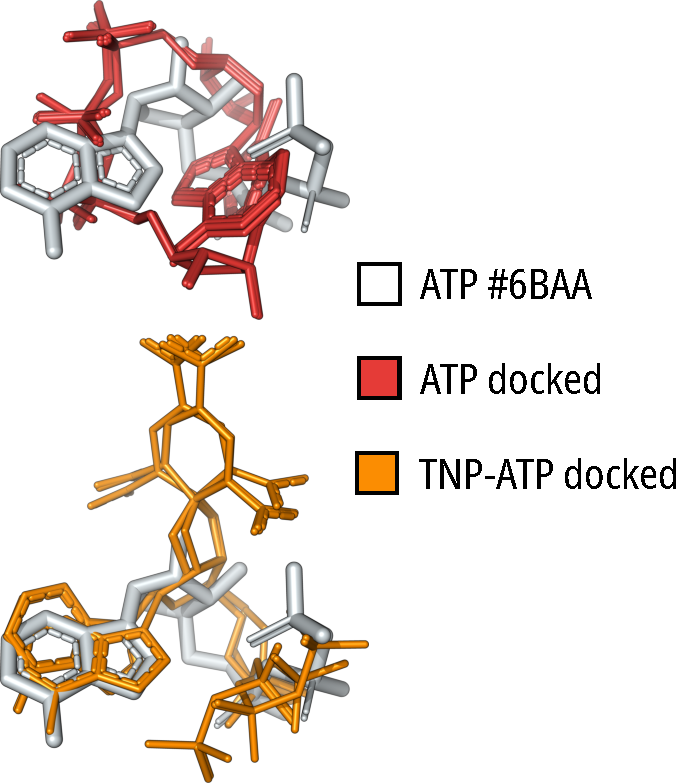
\includegraphics[width=\textwidth]{6baa_docking.pdf}
	\end{subfigure}
	\hfill
	\begin{subfigure}[t]{0.28\textwidth}
		\caption{}\label{ch3fig:6c3p_docking}
		\centering
		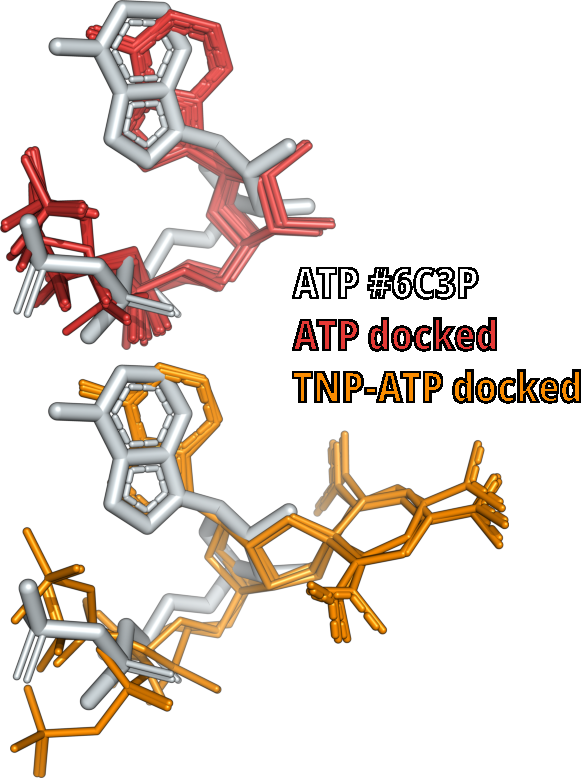
\includegraphics[width=\textwidth]{6c3p_docking.pdf}
	\end{subfigure}
	\hfill
	\begin{subfigure}[t]{0.30\textwidth}
		\caption{}\label{ch3fig:6c3o_docking}
		\centering
		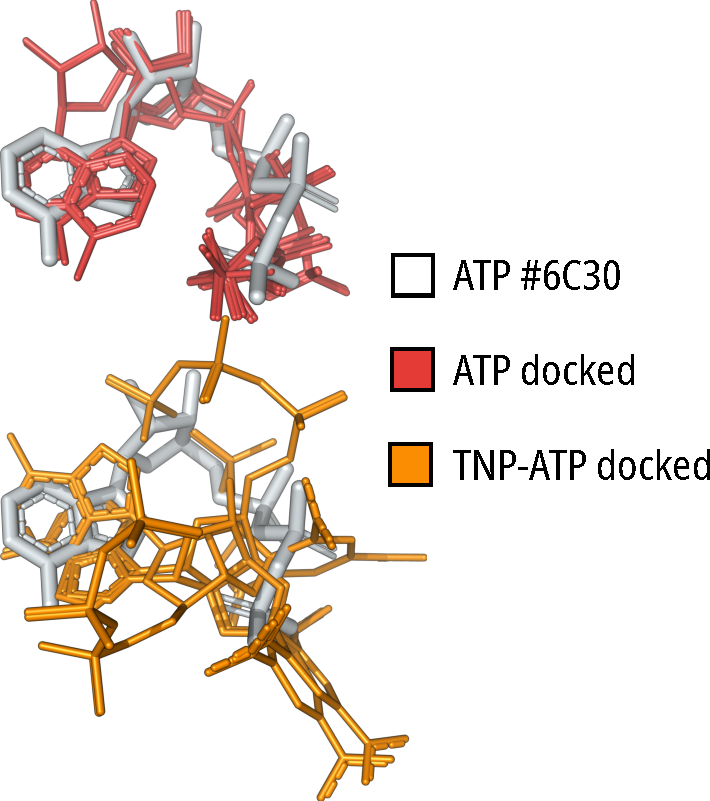
\includegraphics[width=\textwidth]{6c3o_docking.pdf}
	\end{subfigure}
	\vfill
	\begin{subfigure}[t]{0.4\textwidth}
		\caption{}\label{ch3fig:6c3p_bound}
		\centering
		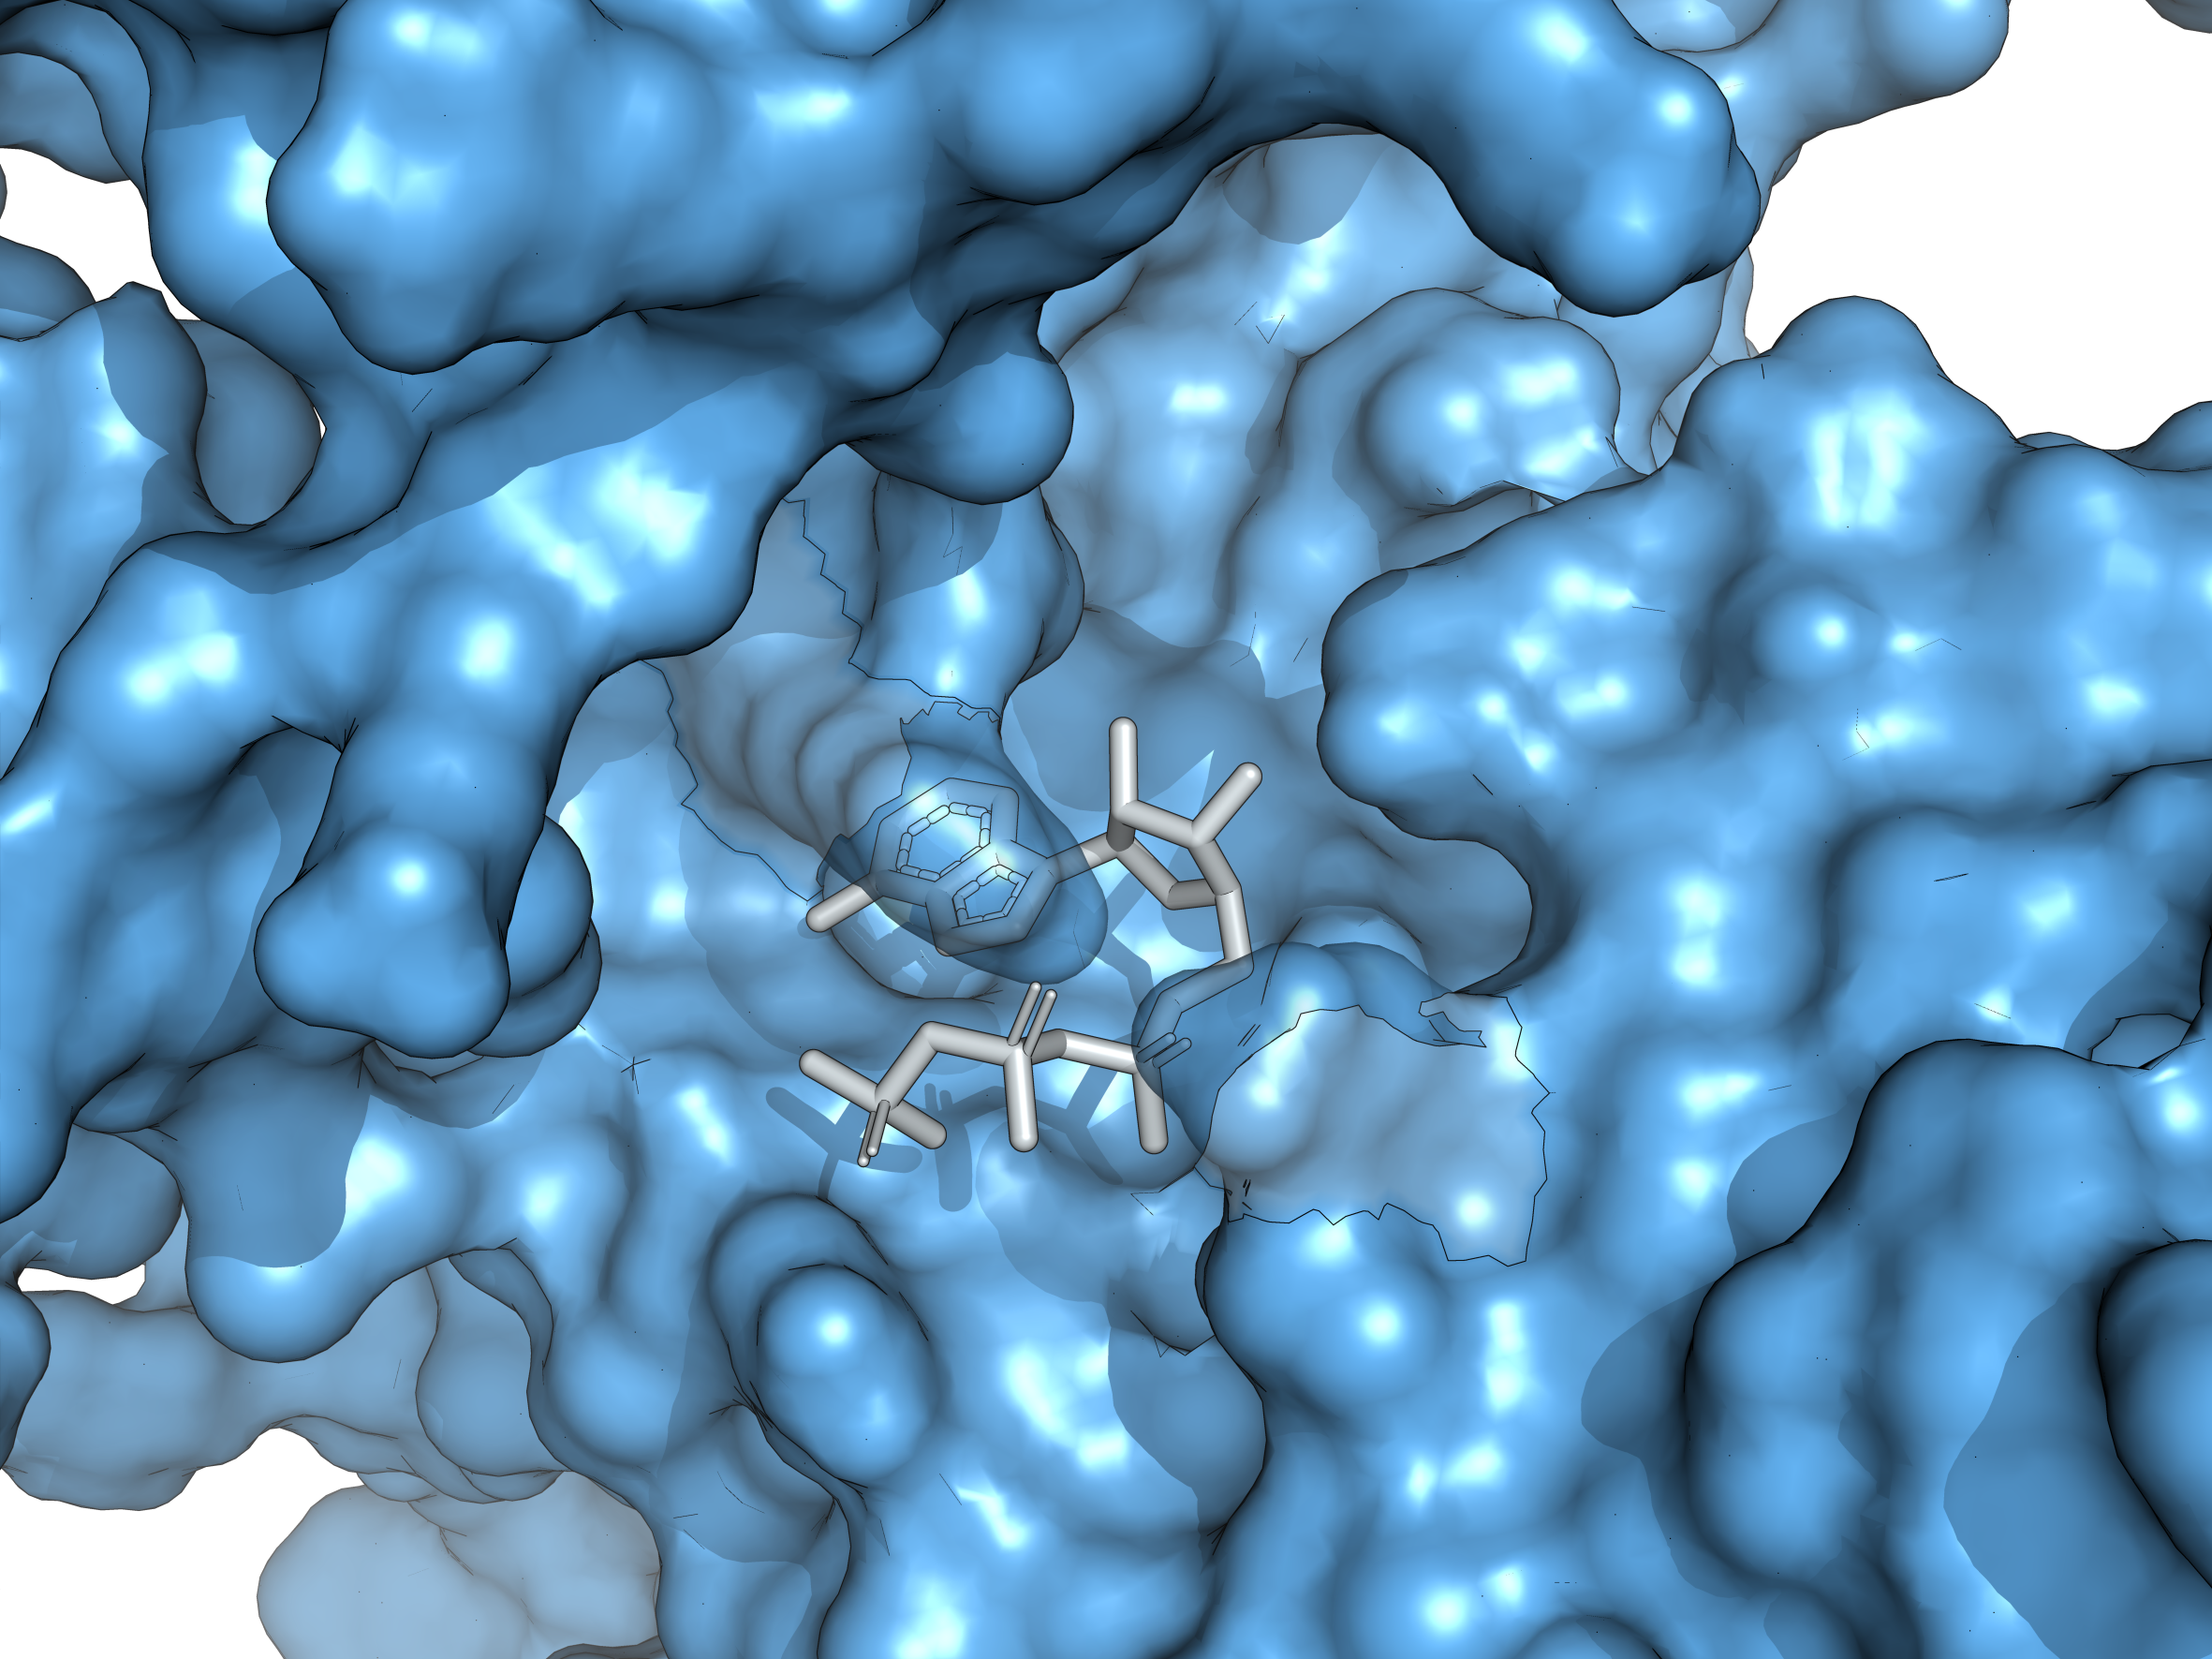
\includegraphics[width=\textwidth]{6c3p_site_bound.png}
	\end{subfigure}
	\hfill
	\begin{subfigure}[t]{0.4\textwidth}
		\caption{}\label{ch3fig:6c3p_docked}
		\centering
		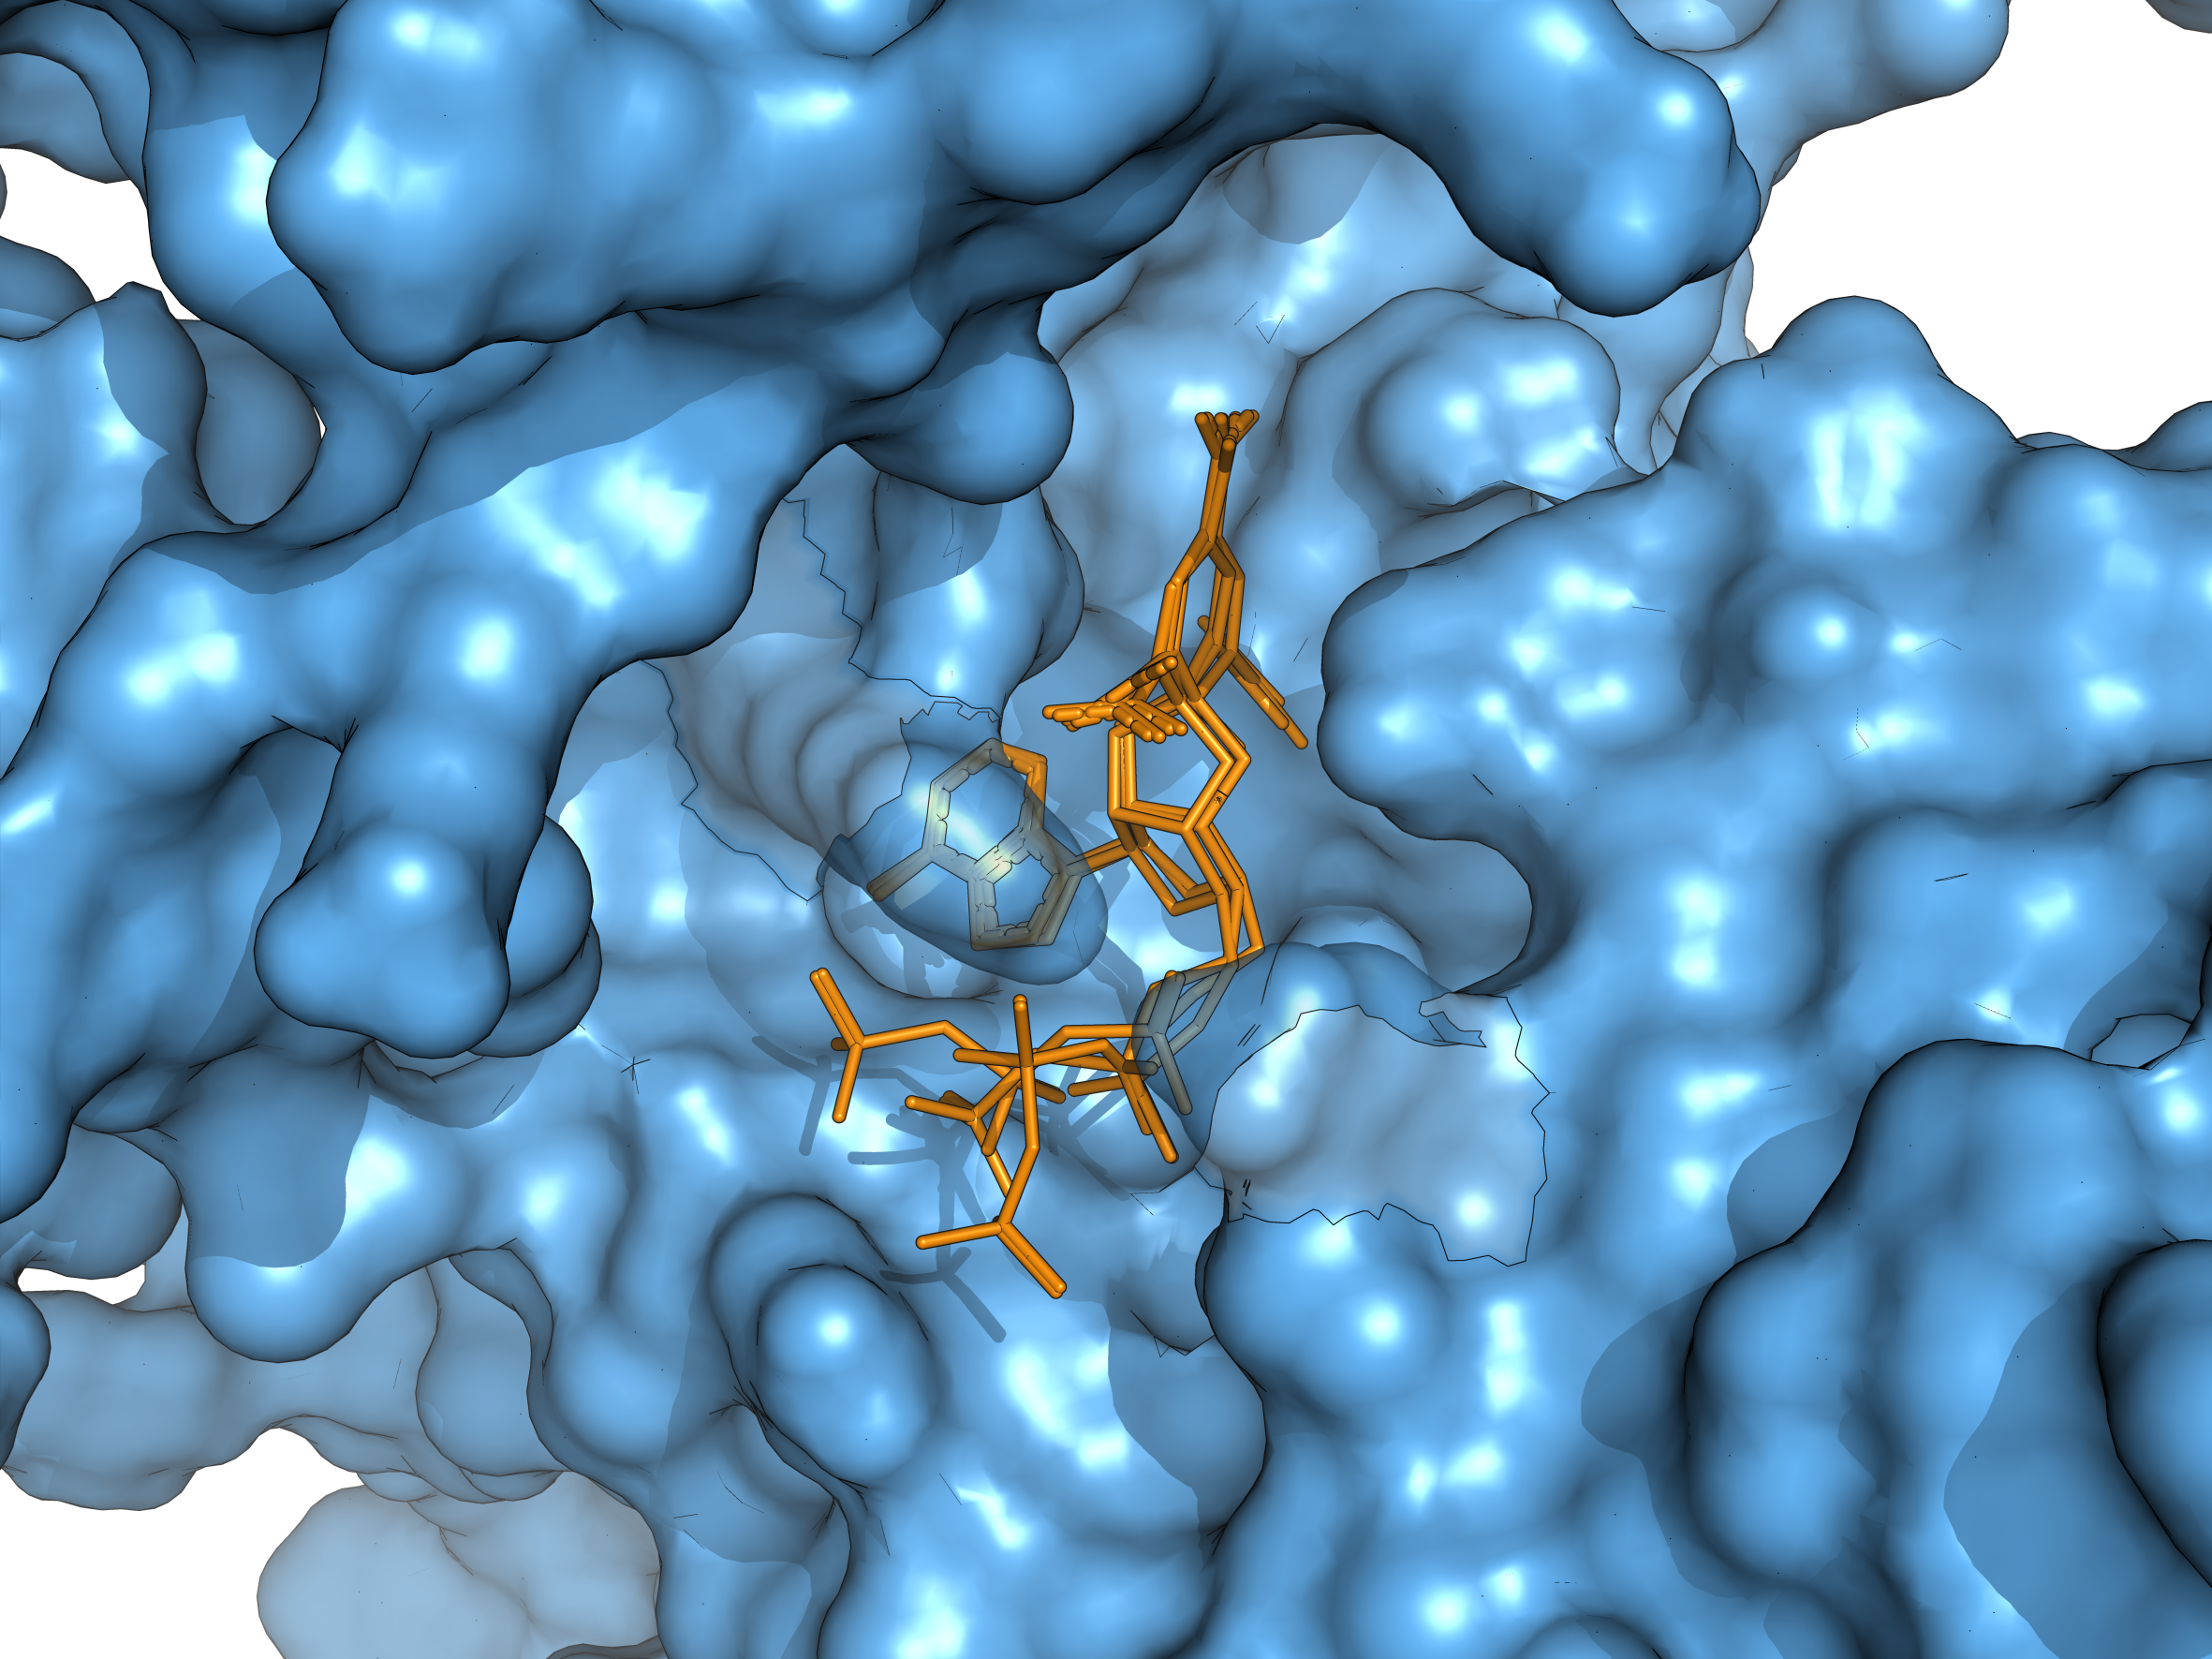
\includegraphics[width=\textwidth]{6c3p_site_docked.png}
	\end{subfigure}
	
	\caption[TNP-nucleotides can bind with a similar pose to ATP]{
	\subref{ch3fig:6baa_docking}, \subref{ch3fig:6c3p_docking}, \subref{ch3fig:6c3o_docking} Cryo-EM binding poses for ATP bound to Kir6.2 (white) overlayed with either the ten highest scoring computationally docked ATP poses (red) or the three highest scoring computationally docked TNP-nucleotide poses (orange).
	Starting poses for ATP were generated from ten different random seeds based on the cryo-EM poses.
	Starting poses for TNP-nucleotides were generated from eleven structures taken from the RCSB database for different proteins solved in the presence of TNP-ATP.
	The poses shown are from \#3B5J (X-ray diffraction structure of TNP-ADP bound to the NBD complex of a bacterial ABC transporter) and \#5SVQ (X-ray diffraction structure of TNP-ATP bound to the human P2X3 ion channel).
	\subref{ch3fig:6c3p_bound} Cryo-EM structure of the nucleotide binding site in the presence of ATP from \#6C3P.
	\subref{ch3fig:6c3p_docked} As \subref{ch3fig:6c3p_bound} but with the three top scoring binding poses for docked TNP-nucleotides.
	}\label{ch3fig:docking}
\end{figure}

\section{Incorporating ANAP into the Kir6.2 binding site}

\subsection{Amber stop codon expression system}

ANAP can be introduced into a protein of interest by essentially expanding the genetic code to incorporate a noncanconical amino acid \cite{chin_expanding_2017}.
The amber stop codon (TAG) is the least frequently occuring stop codon in eukaryotic cells \cite{cridge_eukaryotic_2018}, and can be repurposed to encode ANAP.
This requires the introduction of a transfer RNA (tRNA) which recognises the TAG codon, and an aminoacyl-tRNA synthetase (aaRS) which selectively aminoacylates the tRNA with ANAP into the heterologous expression system , without crossreacting with the existing translational machinery \cite{lee_genetic_2009, chatterjee_genetically_2013}.

\citeauthor{lee_genetic_2009} used directed evolution to develop a tRNA/aaRS pair to encode ANAP in \textit{Saccharomyces cerevisiae} \cite{lee_genetic_2009}.
Briefly, they altered the specificity of \textit{Escherichia coli} leucyl-tRNA synthetase so that it was able to aminoacylate the leucyl-tRNA with ANAP, and not endogenous amino acids.
The coevolved tRNA/aaRS pair were built into an expression plasmid pANAP (Figure \ref{ch3fig:amber_codon}) which is capable of driving expression in mammalian cells \cite{chatterjee_genetically_2013}.
HEK293 cells transfected with pANAP and a plasmid encoding GFP with an amber stop codon at residue position 40 (40TAG) exhibited green fluorescence only when incubated in the presence of ANAP in the culture media \cite{chatterjee_genetically_2013}, demonstrating that ANAP can be selectively incorporated into proteins in mammalian cells.

As far as we are aware, only two other studies have incorporated unnatural amino acids into Kir6.2 \cite{zhang_conserved_2015, devaraneni_structurally_2015}.
\citeauthor{zhang_conserved_2015} incorporated three unnatural tryptophan variants at position W68 to highlight the necessity of a planar amino acid side-chain at this location to maintain physiological K\ATP{} channel function \cite{zhang_conserved_2015}.
However, in this study \textit{Xenopus} oocytes were the heterologous expression system, so rather than transfecting a combination of plasmids, the authors injected a combination of transcribed mRNAs.

\citeauthor{devaraneni_structurally_2015} incorporated azidophenylalanine (AzF) at three different positions on the N-terminus of Kir6.2 (residue numbers 12, 18 and 52) \cite{devaraneni_structurally_2015}.
AzF is photocross-linkable upon exposure to UV light, and the authors used this phenomenon to investigate the extent of physical interactions between the N-terminus of Kir6.2 and SUR1, and how these interactions are mediated by pharmacological chaperones.
In this study, COSm6 cells were the heterologous expression system, and expression of AzF containing constructs was found to be dramatically reduced when compared to wild-type channels.

\subsection{ANAP incorporation into amber stop codon containing constructs}

\begin{figure}[h]
	\centering
	\begin{subfigure}[t]{0.9\textwidth}
		\caption{}\label{ch3fig:amber_codon}
		\centering
		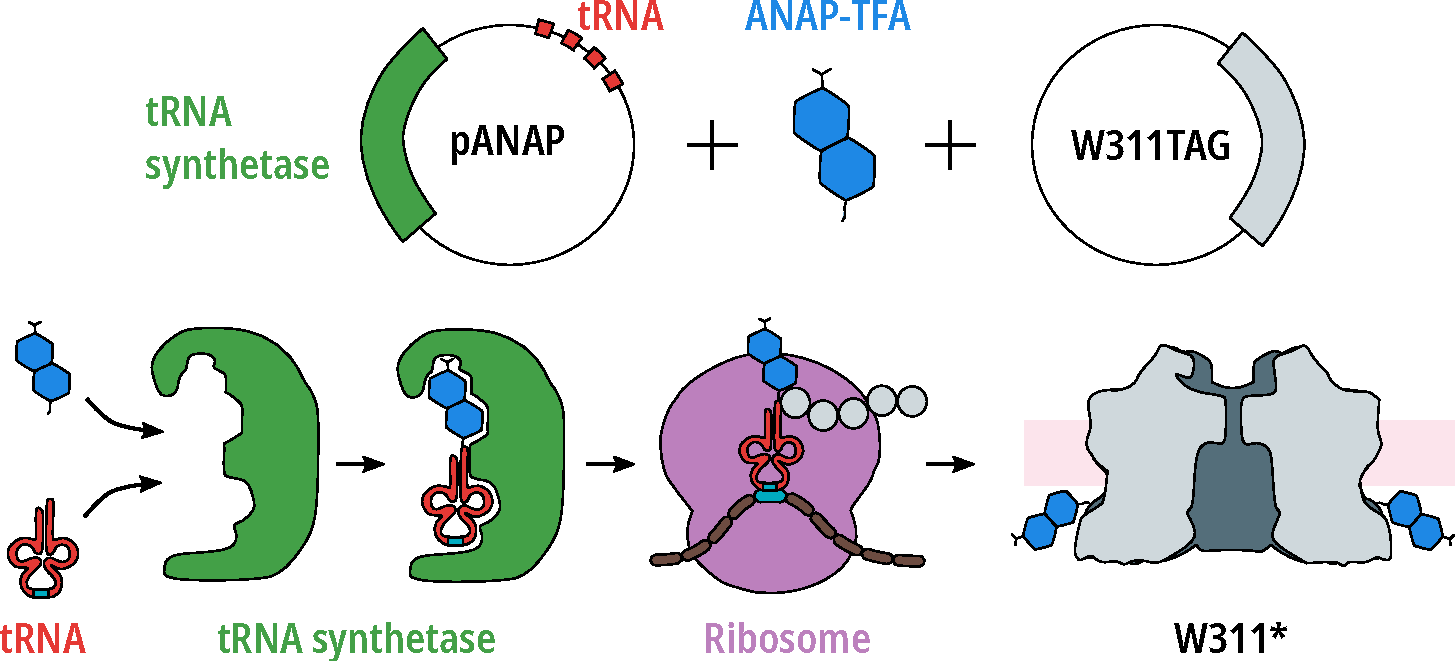
\includegraphics[width=\textwidth]{amber_codon.pdf}
	\end{subfigure}
	\vfill
	\begin{subfigure}[t]{0.45\textwidth}
		\caption{}\label{ch3fig:western_1}
		\centering
		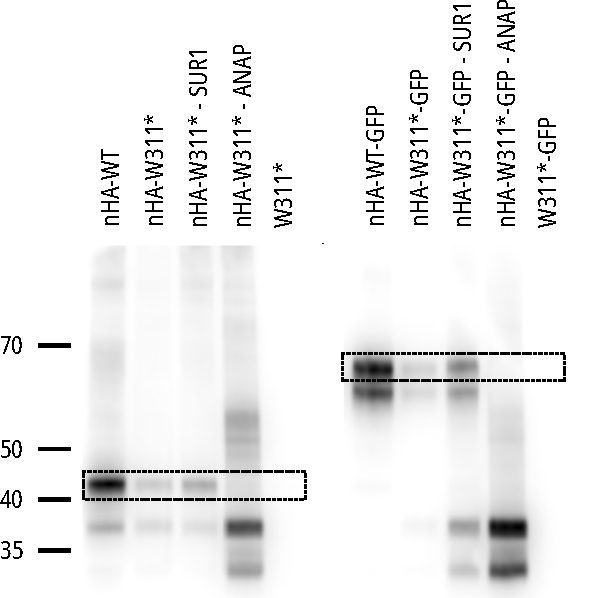
\includegraphics[width=\textwidth]{western_1.pdf}
	\end{subfigure}
	\hfill
	\begin{subfigure}[t]{0.45\textwidth}
		\caption{}\label{ch3fig:western_2}
		\centering
		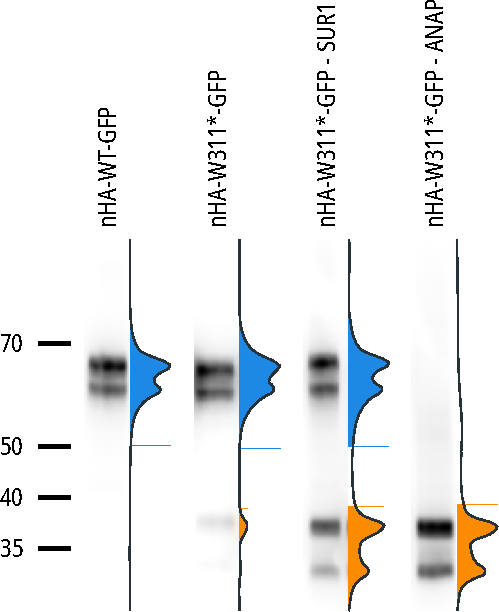
\includegraphics[width=\textwidth]{western_2.pdf}
	\end{subfigure}
	\caption[ANAP incorporation]{
	\subref{ch3fig:amber_codon} ANAP incorporation is accomplished through the transfection of two plasmids.
	pANAP codes for tRNA (red) and it's tRNA synthetase (green), while pW311TAG codes for Kir6.2 with an amber stop codon (TAG) inserted in place of the codon for W311 (grey).
	When the transfected cells are incubated with ANAP (present here as its free acid, ANAP-TFA, blue) the tRNA synthetase assembles tRNA which is capable of recognising the amber stop codon and loads it with ANAP.
	During translation of W311TAG, the primed ANAP tRNAs recognise the TAG and insert ANAP into the desired location.
	\subref{ch3fig:western_1} Two separate western blots against the N-terminal HA epitope incorporated into WT or W311* (left) and WT-GFP or W311*-GFP (right) constructs.
	Cells were co-transfected with pANAP, eRF1-E55D, and SUR1 unless otherwise indicated.
	Full-length Kir6.2 constructs are indicated on each gel with a dashed box.
	The doublets represent an N-terminally truncated product decribed in the main text.
	\subref{ch3fig:western_2} Each lane from the gel containing C-terminally GFP-tagged consstructs is displayed normalised to its highest intensity accompanied by the line averaged density trace.
	The density peak corresponding to full-length Kir6.2 is filled in blue.
	The density peak for C-terminally truncated Kir6.2 is filled in orange.
	}\label{ch3fig:anap_incorporation}
\end{figure}

The nature of the amber stop codon suppression system requires a number of careful controls to ensure the following:

\begin{enumerate}
	\item Stop codon recognition is not perfect, and there is a chance of read-through.
	Instead of incorporating ANAP, it is possible that the translation machinery can insert endogenous amino acids instead, leading to production of full length,unlabelled Kir6.2.
	However, we found that cells transfected with W311TAG constructs and pANAP which were not cultured in the presence of ANAP did not produce full length Kir6.2 (Figure \ref{ch3fig:western_1}, \ref{ch3fig:western_2}), suggesting there is minimal read-through of the stop codon in our experiments.
	\item Introducing a stop codon creates a risk that truncated Kir6.2 will be produced instead of ANAP labelled Kir6.2.
	This risk can be reduced by transfecting a dominant negative engineered version of eukaryotic translation termination factor 1(eRF1-E55D), which does not efficiently terminate protein synthesis in response to the amber stop codon (but leaves opal and ochre stop codons nearly unaffected) and thus increases the incorporation of ANAP \cite{schmied_efficient_2014}.
	We found that transfection of W311TAG constructs with a C-terminal GFP tag produced minimal truncated Kir6.2 (less than \SI{10}{\percent} of the total density observed in Figure \ref{ch3fig:western_2}).
	\item Despite being the least frequent eukaryotic stop codon, the amber stop codon is still present in a significant number of proetin sequences.
	We must be careful that ANAP is not incorporated into a protein which localises to the plasma membrane to an extent which would affect our ability to assign ANAP fluorescence to Kir6.2.
	We found that in cells transfected with GFP-tagged Kir6.2 without an amber stop codon, there was no increase in ANAP fluorescence at the cell membrane (Figure \ref{ch3fig:wt_confocal}, \ref{ch3fig:wt_confocal_profiles}).
	By contrast, when W311TAG-GFP was transfected, we saw a clear increase in ANAP fluorescence at the cell membrane (Figure \ref{ch3fig:w311_confocal}, \ref{ch3fig:w311_confocal_profiles}), suggesting that any observed ANAP fluorescence at the cell membrane originates from our labelled Kir6.2 construct.
\end{enumerate}

\begin{figure}[h]
	\centering
	\begin{subfigure}[t]{0.55\textwidth}
		\caption{}\label{ch3fig:wt_confocal}
		\centering
		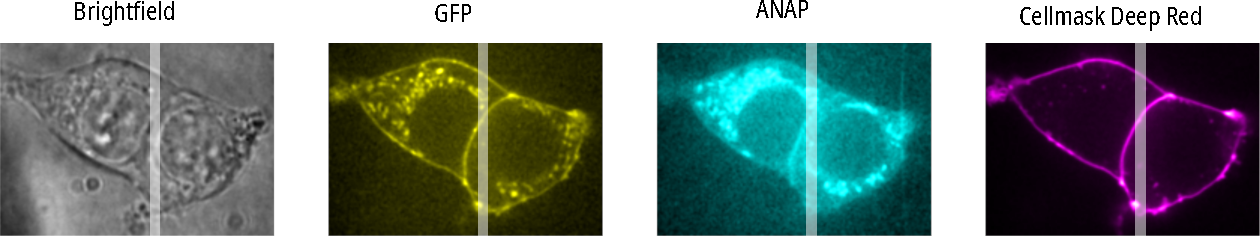
\includegraphics[width=\textwidth]{wt_confocal.pdf}
	\end{subfigure}
	\hfill
	\begin{subfigure}[t]{0.35\textwidth}
		\caption{}\label{ch3fig:wt_confocal_profiles}
		\centering
		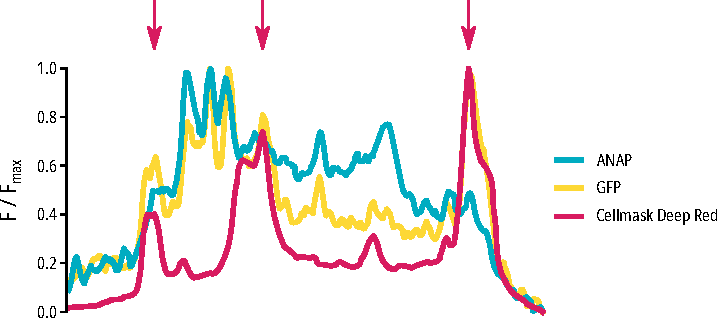
\includegraphics[width=\textwidth]{wt_confocal_profiles.pdf}
	\end{subfigure}
	\vfill
	\begin{subfigure}[t]{0.55\textwidth}
		\caption{}\label{ch3fig:w311_confocal}
		\centering
		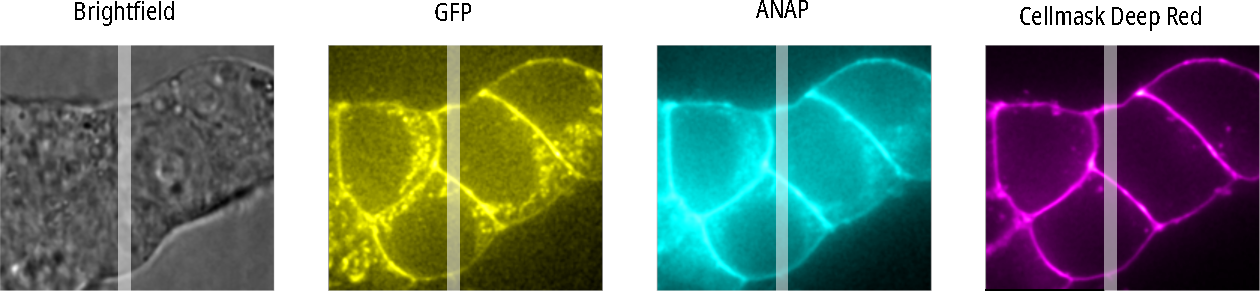
\includegraphics[width=\textwidth]{w311_confocal.pdf}
	\end{subfigure}
	\hfill
	\begin{subfigure}[t]{0.35\textwidth}
		\caption{}\label{ch3fig:w311_confocal_profiles}
		\centering
		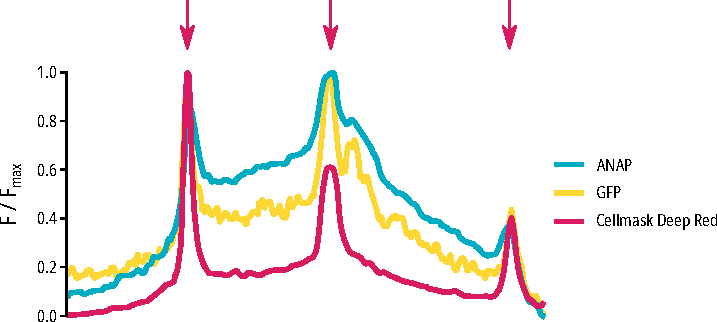
\includegraphics[width=\textwidth]{w311_confocal_profiles.pdf}
	\end{subfigure}
	\caption[Confocal imaging]{
	\subref{ch3fig:wt_confocal}, \subref{ch3fig:w311_confocal} Confocal images of two HEK293T cells transfected with WT-GFP (\subref{ch3fig:wt_confocal}) or W311TAG-GFP (\subref{ch3fig:w311_confocal}), plus SUR1, pANAP, peRF1-E55D and with ANAP in the culture medium.
	Cells were incubated with Cellmask Deep Red for ten minutes before imaging to label the plasma membranes.
	The vertical grey box indicates the section of the images plotted in \subref{ch3fig:wt_confocal_profiles} and \subref{ch3fig:w311_confocal_profiles}
	Images are displayed after median filtering with a box radius of 5, and normalising the intensities per channel.
	\subref{ch3fig:wt_confocal_profiles}, \subref{ch3fig:w311_confocal_profiles}The line-averaged intensity of the pixels in the grey boxes in \subref{ch3fig:wt_confocal} and \subref{ch3fig:w311_confocal} respectively.
	The plasma membranes are identifiable as clear peaks in the Cellmask Deep Red fluorescence (magenta) and are marked with arrows.
	Notably, while there are clear GFP peaks at the membrane in both \subref{ch3fig:wt_confocal_profiles} and \subref{ch3fig:w311_confocal_profiles}, only in \subref{ch3fig:w311_confocal_profiles} do peaks in the ANAP fluorescence coincide with the membrane.
	}
\end{figure}

\section{Testing for functional membrane expression}

\subsection{Surface expression of HA-epitope labelled Kir6.2 constructs}

To assess the ability of ANAP-incorporating constructs to traffic to the plasma membrane, we used a luminence-based surface expression assay.
This assay relies on the recognition of an HA-epitope introduced into an extracellular region of the protein of interest (in this case, the N-terminal region of Kir6.2) by an anti-HA primary antibody followed by an HRP-conjugated secondary antibody.
The luminescence after applying HRP substrate is then proportional to the amount of protein at the plasma membrane of the cells.

We assessed the membrane expression of N-terminally HA-tagged Kir6.2 (nHA-Kir6.2) in the presence or absence of ANAP in the culture media and in the presence or absence of cotransfected SUR1.
We also measured how the addition of a C-terminal GFP tag affected membrane expression under these conditions.
We used untagged Kir6.2 as a control for nonspecific luminesence.

We find that for wild-type Kir6.2 (WT) there is roughly a 20-fold increase in observed luminescence when coexpressed with SUR1 over background, and roughly a 100-fold increase for the C-terminally GFP tagged Kir6.2 (WT-GFP, Figure \ref{ch3fig:surface_expression_1}, \ref{ch3fig:surface_expression_3}).
There is no difference in surface expression of these constructs when ANAP is present in the culture medium (Figure \ref{ch3fig:surface_expression_1}, \ref{ch3fig:surface_expression_4}).
When ANAP is incorporated at either residue 183 or 311 (F183* and W311* respectively) we see an increase in luminescence over background when coexpressed with SUR1 and with ANAP present in the culture medium (Figure \ref{ch3fig:surface_expression_1}, \ref{ch3fig:surface_expression_3}).
The presence of the C-terminal GFP tag increases luminescence further for both constructs, dramatically so for W311*.
However, when F183* is transfected and ANAP is not present in the culture media we still see a similar increase in fluorescence over background when compared to the luminescence when ANAP is present (Figure \ref{ch3fig:surface_expression_1}, \ref{ch3fig:surface_expression_4}), suggesting that a large proportion of the protein reaching the membrane does not have ANAP incorporated.
In contrast, when W311*-GFP is transfected with SUR1 in the presence of ANAP, we see a 10-fold increase in luminescence compared to when ANAP is not present, consitent with the majority of surface expressed protein incorporating ANAP.
We also see a consistent increase in luminescence for all constructs aside from W311* due to cotransfection with SUR1 (Figure \ref{ch3fig:surface_expression_2}), suggesting that the incorporation of ANAP and the addition of a C-terminal GFP tag do not affect the role of SUR1 in forming the full K\ATP{} complex and trafficking to the membrane.

\begin{figure}[h]
	\centering
	\begin{subfigure}[t]{0.45\textwidth}
		\caption{}\label{ch3fig:surface_expression_1}
		\centering
		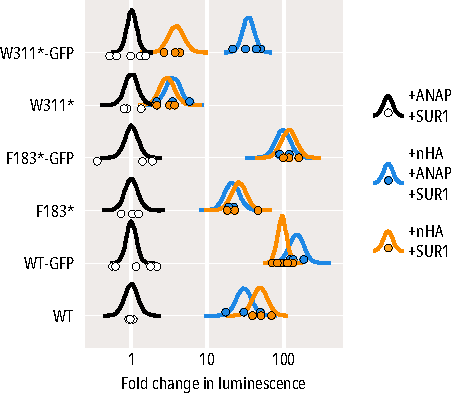
\includegraphics[width=\textwidth]{surface_expression_1.pdf}
	\end{subfigure}
	\hfill
	\begin{subfigure}[t]{0.45\textwidth}
		\caption{}\label{ch3fig:surface_expression_2}
		\centering
		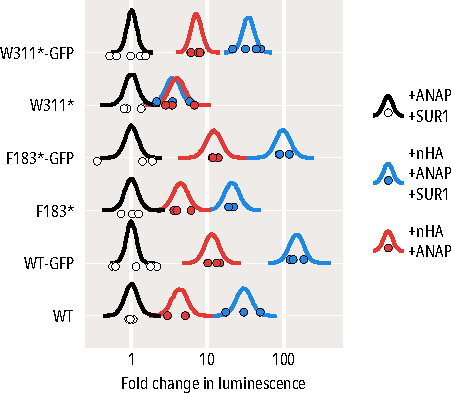
\includegraphics[width=\textwidth]{surface_expression_2.pdf}
	\end{subfigure}
	\vfill
	\begin{subfigure}[t]{0.45\textwidth}
		\caption{}\label{ch3fig:surface_expression_3}
		\centering
		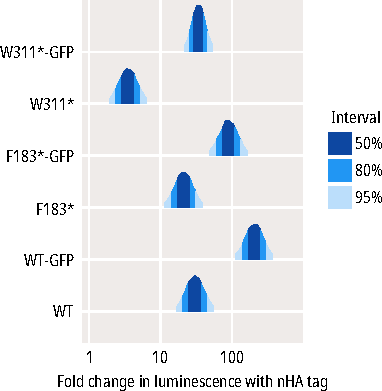
\includegraphics[width=\textwidth]{surface_expression_3.pdf}
	\end{subfigure}
	\hfill
	\begin{subfigure}[t]{0.45\textwidth}
		\caption{}\label{ch3fig:surface_expression_4}
		\centering
		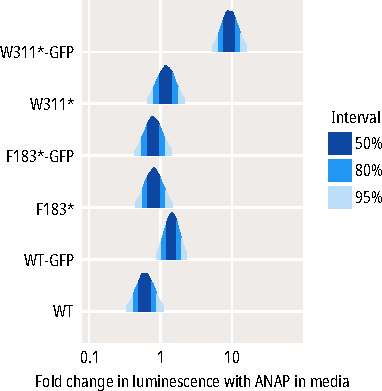
\includegraphics[width=\textwidth]{surface_expression_4.pdf}
	\end{subfigure}
	\caption[ANAP construct surface expression assay]{
	\subref{ch3fig:surface_expression_1}, \subref{ch3fig:surface_expression_2} Individual observations (points) and posterior probability distributions for surface expression of Kir6.2 constructs.
	Before fitting, the observations for each construct were centered by subtracting the mean of the luminesence observed without the N-temrinal HA tag.
	Observations for constructs without the N-terminal HA tag and for constructs transfected with both ANAP and SUR1 are duplicated between panels to clarify the differences observed when either ANAP (\subref{ch3fig:surface_expression_1}) or SUR1 (\subref{ch3fig:surface_expression_2}) are omitted.
	\subref{ch3fig:surface_expression_3}, \subref{ch3fig:surface_expression_4} Contrasts between constructs differing only in the presence or absence of the N-terminal HA-tag (\subref{ch3fig:surface_expression_3}) or the presence or absence of ANAP in the culture media (\subref{ch3fig:surface_expression_4}).
	Different intervals in the posterior probability distribution of the contrasts are shown in shades of blue.
	}
\end{figure}

\subsection{Electrophysiology of Kir6.2 constructs}

To establish whether W311*-GFP formed K\ATP{} channels with similar function to wild-type, we excised patches from cells transfected with either WT-GFP or W311*-GFP cotransfected with SUR1.
Excision was performed in Mg\textsuperscript{2+}-free solution to reduce rundown and to prevent activation of the channel by nucleotides.
We observed similar magnitudes of current for both WT-GFP and W311*-GFP, and currents ran own at similar rates.

We fit our inhibition data with equation \ref{eq:hill} (Figure \ref{ch3fig:atp_inhibition_1}) as described in the methods.
Briefly, our fitting procedure assumes that there is a population parameter for $IC_{50}$, $I_{max}$ and $h$, and an additional 'random' effect on $IC_{50}$ that can differ between experiments (shown in Figure \ref{ch3fig:atp_inhibition_2}).
Our fits result in posterior probability distributions for the population $IC_{50}$ parameter shown in blue in Figure \ref{ch3fig:ec50_fits_1}.
These distributions reflect our confidence in the population parameter for the $IC_{50}$, marginalising over the random effect of different experiments.
For all $IC_50$ and $EC_{50}$ values fitted this way, in the text we will report the \SI{95}{\percent} intervals of the posterior probability distribution for the fitted population parameter.

Perfusion of ATP resulted in current inhibition with an IC\textsubscript{50} of \SIrange{24}{45}{\micro\Molar} for WT-GFP+SUR1 and \SIrange{75}{124}{\micro\Molar} for W311*-GFP+SUR1.
Thus, despite the distance from the ATP binding site, the incorporation of ANAP at W311 clearly affects some aspect of nucleotide inhibition.
However, we assume that insights into the function of the ANAP-incorporating channel will still be applicable to wild-type channels despite the change in nucleotide inhibition.

Next, we established that TNP-ATP inhibits K\ATP{} (Figure \ref{ch3fig:tnpatp_inhibition_1}, \ref{ch3fig:tnpatp_inhibition_2}).
We observed current inhibition with an IC\textsubscript{50} of \SIrange{0.7}{1.8}{\micro\Molar} for WT-GFP+SUR1 and \SIrange{2.9}{10}{\micro\Molar} for W311*-GFP+SUR1.
K\ATP{} thus appears to be more sensitive to inhibition by TNP-ATP than by ATP.
This could potentially be due to extra contacts made by the TNP moiety with Kir6.2, seen in our computational docking (Figure \ref{ch3fig:docking}).

\begin{figure}[h]
	\centering
	\begin{subfigure}[t]{0.45\textwidth}
		\caption{}\label{ch3fig:atp_inhibition_1}
		\centering
		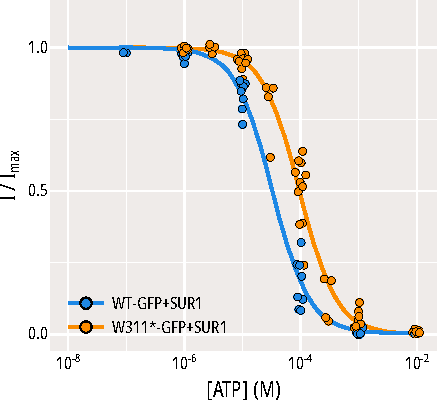
\includegraphics[width=\textwidth]{atp_inhibition_1.pdf}
	\end{subfigure}
	\hfill
	\begin{subfigure}[t]{0.45\textwidth}
		\caption{}\label{ch3fig:tnpatp_inhibition_1}
		\centering
		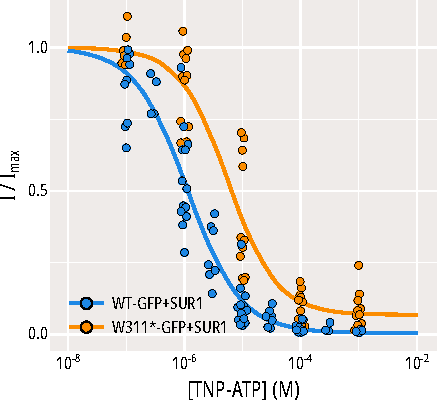
\includegraphics[width=\textwidth]{tnpatp_inhibition_1.pdf}
	\end{subfigure}
	\vfill
	\begin{subfigure}[t]{0.9\textwidth}
		\caption{}\label{ch3fig:atp_inhibition_2}
		\centering
		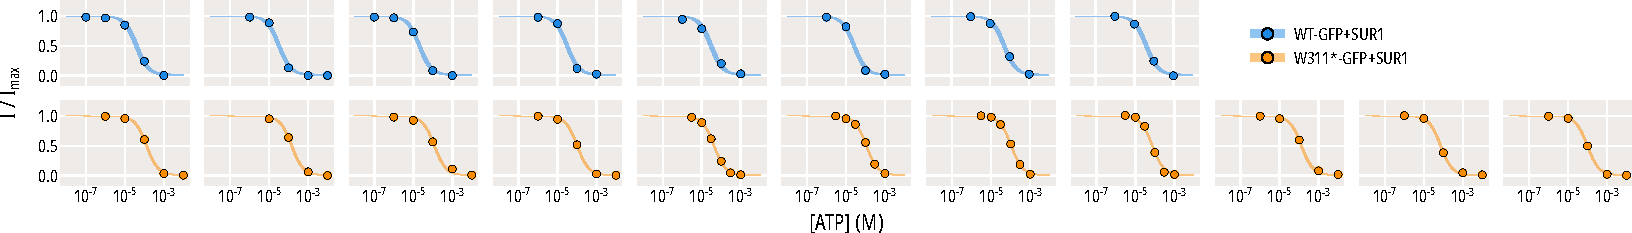
\includegraphics[width=\textwidth]{atp_inhibition_2.pdf}
	\end{subfigure}
	\vfill
	\begin{subfigure}[t]{0.9\textwidth}
		\caption{}\label{ch3fig:tnpatp_inhibition_2}
		\centering
		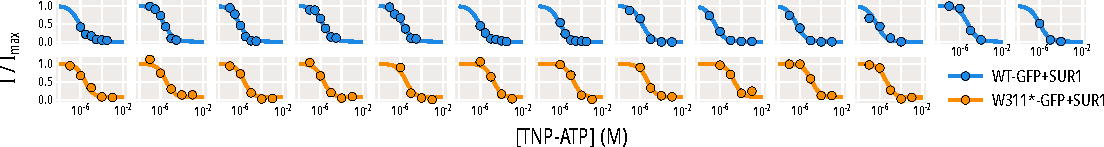
\includegraphics[width=\textwidth]{tnpatp_inhibition_2.pdf}
	\end{subfigure}
	\vfill
	\begin{subfigure}[t]{0.6\textwidth}
		\caption{}\label{ch3fig:ec50_fits_1}
		\centering
		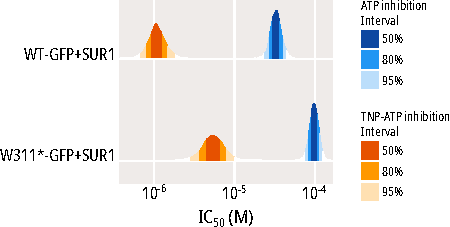
\includegraphics[width=\textwidth]{ec50_fits_1.pdf}
	\end{subfigure}
	\caption[WT-GFP and W311*-GFP electrophysiology]{
	\subref{ch3fig:atp_inhibition_1},  \subref{ch3fig:tnpatp_inhibition_1}Inhibition of current by ATP (\subref{ch3fig:atp_inhibition_1}) or TNP-ATP (\subref{ch3fig:tnpatp_inhibition_1}) in excised patches expressing either WT-GFP+SUR1 (blue) or W311*-GFP+SUR1 (orange).
	Each point represents an individual measurement normalised to the average of the current measured immediately before TNP-ATP perfusion, and immediately after TNP-ATP washout.
	The smooth filled curves are the \SI{95}{\percent} intervals of the posterior probability distribution of fits to equation \ref{eq:hill} as described in the methods.
	\subref{ch3fig:atp_inhibition_2}, \subref{ch3fig:tnpatp_inhibition_2} Data from each experiment is shown separately.
	The smooth filled curves are the \SI{95}{\percent} intervals of the posterior predictions for each experiment.
	\subref{ch3fig:ec50_fits_1} Posterior probability distributions for the population $IC_{50}$ values for inhibition by ATP (blue) or TNP-ATP (orange).
	}
\end{figure}

\subsection{Unroofed membrane binding assay of Kir6.2 constructs}

We then directly measured nucleotide binding to W311*-GFP in unroofed membranes.
Briefly sonicating transfected cells adhered to coverslips results in the lower membrane of the cell remaining stuck to the coverslip while the rest of the cell contents is disrupted and perfused away.
This leaves the cytoplasmic domains of expressed K\ATP{} channels open to perfusion of TNP-ATP.
These patches of membrane are barely visible under brightfield illumination, but due to the presence of the C-terminal GFP tag and the incorporated ANAP, we can see patches of membrane expressing K\ATP{} channels light up when we excite either fluorophore (Figure \ref{ch3fig:unroofed_images}).
By measuring the fluorescence spectra of patches of unroofed membrane, we can separate the fluorescence emission peaks of the C-terminal GFP tag and the incorporated ANAP (Figure \ref{ch3fig:unroofed_spectral_images}).
The peak at \SI{472}{\nano\metre} corresponds to ANAP emission, while the peak at \SI{508}{\nano\metre} corresponds to GFP emission.
We observed no change in the locations of those peaks in the presence of ATP or TNP-ATP.

Perfusing TNP-ATP results in a decrease in the peak corresponding to ANAP fluorescence, and a concomittant increase in a fluorescence peak which corresponds to the TNP-ATP (Figure \ref{ch3fig:unroofed_spectral_traces}).
This phenomenon is the fresult of FRET between TNP-ATP bound to the channel at the Kir6.2 binding site.
The decrease in ANAP fluorescence is almost directly correlated to an increase in bound nucleotide.
We chose to measure the decrease in ANAP fluorescence rather than the increase in TNP-ATP fluorescence or the change in the ratio of ANAP:TNP-ATP fluorescence as we know that the ANAP fluorescence is specific to the Kir6.2 binding site.
Increases in TNP-ATP fluorescence could in part be due to direct excitation of TNP-ATP bound to other membrane proteins.
We can plot the quenching of ANAP fluorescence as a concentration-response curve as in Figure \ref{ch3fig:unroofed_intensities}.

\begin{figure}[h]
	\centering
	\begin{subfigure}[t]{0.3\textwidth}
		\caption{}\label{ch3fig:unroofed_images}
		\centering
		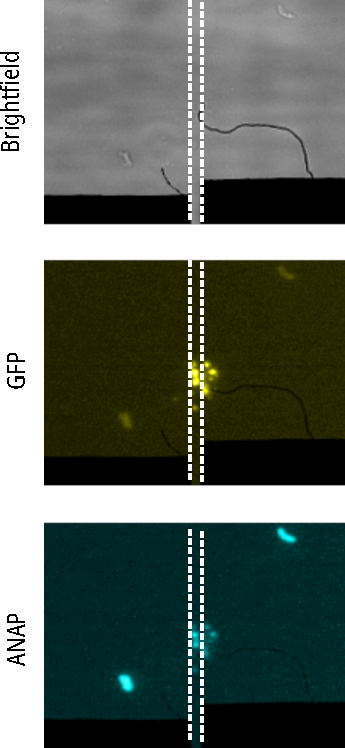
\includegraphics[width=\textwidth]{unroofed_images.pdf}
	\end{subfigure}
	\hfill
	\begin{subfigure}[t]{0.6\textwidth}
		\caption{}\label{ch3fig:unroofed_spectral_images}
		\centering
		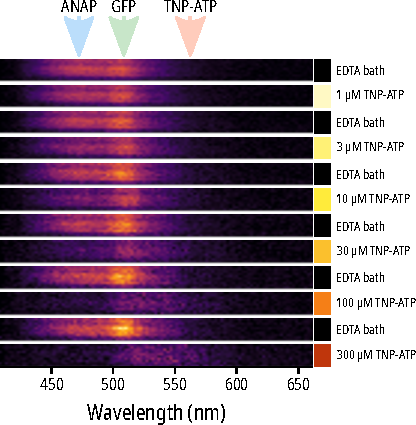
\includegraphics[width=\textwidth]{unroofed_spectral_images.pdf}
	\end{subfigure}
	\vfill
	\begin{subfigure}[t]{0.45\textwidth}
		\caption{}\label{ch3fig:unroofed_spectral_traces}
		\centering
		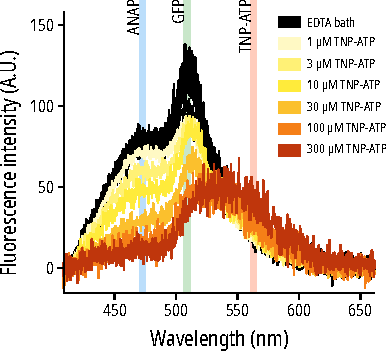
\includegraphics[width=\textwidth]{unroofed_spectral_traces.pdf}
	\end{subfigure}
	\hfill
	\begin{subfigure}[t]{0.45\textwidth}
		\caption{}\label{ch3fig:unroofed_intensities}
		\centering
		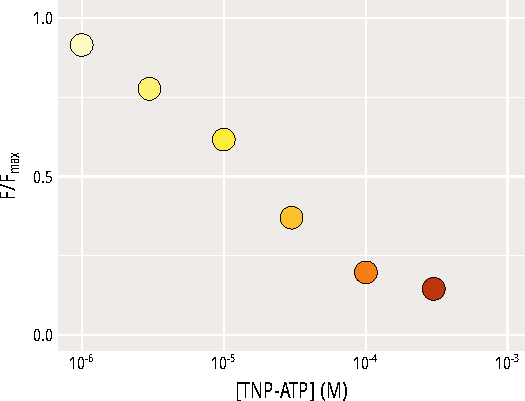
\includegraphics[width=\textwidth]{unroofed_intensities.pdf}
	\end{subfigure}
	\caption[Unroofed membranes spectral images]{
	\subref{ch3fig:unroofed_images} An unroofed membrane patch imaged either with brightfield illumination (top panel), GFP fluorescence (middle panel) or ANAP fluorescence (bottom panel).
	The dashed white lines indicate the region of the image isolated by the spectrometer mask for spectral imaging.
	\subref{ch3fig:unroofed_spectral_images} Bleaching-corrected spectral images of the unroofed membrane patch in \subref{ch3fig:unroofed_images} captured in the presence of different concentrations of TNP-ATP.
	Each image represents the region delineated by the dashed white lines in \subref{ch3fig:unroofed_images}, but the $x$-dimension is lost and instead we are able to separate the emitted light by wavelength.
	\subref{ch3fig:unroofed_spectral_traces} Line-averaged, bleaching-corrected traces of the spectral images in \subref{ch3fig:unroofed_spectral_images} coloured according to the TNP-ATP concentration present.
	The two clearest peaks in emission belong to ANAP and GFP.
	The ANAP peak is marked with with a grey line.
	At the higher TNP-ATP concentrations, the presence of a third peak belonging to the TNP-moiety begins to appear as the ANAP peak reduces in intensity due to FRET.
	\subref{ch3fig:unroofed_intensities} Bleaching-corrected ANAP fluorescence intensities of the spectral traces in \subref{ch3fig:unroofed_spectral_images} expressed as the average fluorescence of the ANAP peak (the average intensity of the spectra inside the grey line in \subref{ch3fig:unroofed_spectral_images}) divided by the average fluorescence of the ANAP peak in $0$ TNP-ATP, or $F/F_{max}$.
	}
\end{figure}

Before analysis, ANAP bleaching was corrected as shown in Figure \ref{ch3fig:bleaching_plots_2}.
ANAP intensities of spectra imaged during bath perfusion in between applications of TNP-ATP were fit with Equation \ref{eq:bleaching}.
We found that all unroofed experiments showed bleaching well described by the single exponential fit to equation \ref{eq:bleaching}.
In each experiment, there was a mean proportion of \SI{49}{\percent} ANAP fluorescence remaining by the last exposure (Figure \ref{ch3fig:bleaching_terms_4}), maintaining a good signal-to-noise ratio for each spectra imaged.

\begin{figure}[h]
	\centering
	\begin{subfigure}[t]{0.9\textwidth}
		\caption{}\label{ch3fig:bleaching_plots_2}
		\centering
		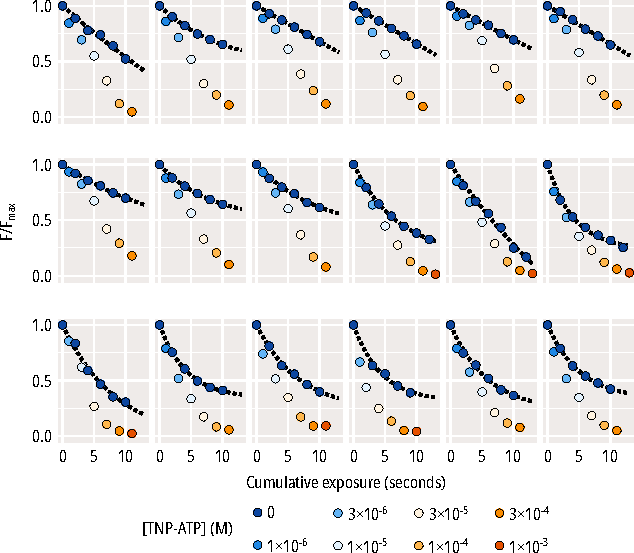
\includegraphics[width=\textwidth]{bleaching_plots_2.pdf}
	\end{subfigure}
	\vfill
	\begin{subfigure}[t]{0.45\textwidth}
		\caption{}\label{ch3fig:bleaching_terms_3}
		\centering
		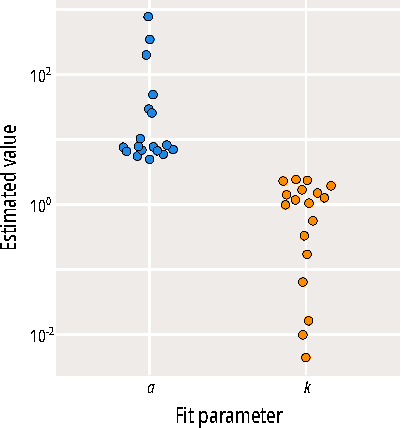
\includegraphics[width=\textwidth]{bleaching_terms_3.pdf}
	\end{subfigure}
	\hfill
	\begin{subfigure}[t]{0.45\textwidth}
		\caption{}\label{ch3fig:bleaching_terms_4}
		\centering
		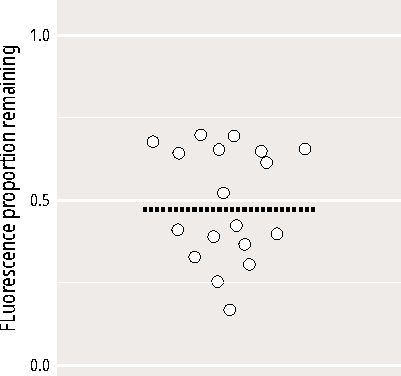
\includegraphics[width=\textwidth]{bleaching_terms_4.pdf}
	\end{subfigure}
	\caption[Unroofed membranes bleaching correction]{
	\subref{ch3fig:bleaching_plots_2} Normalised ANAP fluorescence intensities in unroofed membranes perfused at different concentrations of TNP-ATP are shown as points coloured according to the concentration of TNP-ATP.
	The black dashed lines are fits to the fluorescence intensities without TNP-ATP present with equation \ref{eq:bleaching}.
	\subref{ch3fig:bleaching_terms_3} Values of the two parameters in equation \ref{eq:bleaching} for fits to each of the experiments in \subref{ch3fig:bleaching_plots_2}.
	Estimates are shown on a log scale due to a number of the experiments which show bleaching behaviour on a different timescale than the majority.
	\subref{ch3fig:bleaching_terms_4} Proportion of ANAP fluorescence remaining unbleached in the last exposure taken without the presence of TNP-ATP in each experiment.
	The dashed line is the mean, with a value of $0.49$.
	}
\end{figure}

While our measurements of ANAP quenching are proportional to nucleotide binding to K\ATP{}, the raw $F/F_{max}$ observations are not directly equivalent to the unbound fraction of Kir6.2 subunits.
This non-equivalence is due to two factors.
Firstly, there is the potential for crosstalk between ANAP incorporated in one subunit and TNP-ATP bound to the adjacent subunits.
To determine the extent to which this crosstalk would affect the measured FRET efficiency when ANAP is incorporated at position 311, we adapted a program described by \citeauthor{deplazes_exifret_2012} which uses a numerical method to model FRET in complex geometries.
We implemented a simple version of this program in Python which uses a Monte Carlo simulation scheme to approximate the observed FRET efficiency for a given set of donor and acceptor fluorophores and coordinates.
An overview of the program is shown in Figure \ref{ch3fig:exifret_program}.
We did not measure the fluorescence lifetimes and quantum yields of ANAP and TNP-ATP directly, instead using previously determined values \cite{zagotta_measuring_2016-1, ye_spectroscopic_1999, ishikawa_single-molecule_2002}.
The fluorescence lifetime of TNP-ATP differs when it is bound to proteins; we ran simulations using the fluorescence lifetime of TNP-ATP in solution and the fluorescence lifetime of bound TNP-ATP and saw no difference in the FRET efficiency.

We simulated the expected FRET for a single K\ATP{} channel bound to 0-4 molecules of TNP-ATP in two different scenarios.
In the idealised scenario, each ANAP molecule is only able to FRET with the TNP-ATP molecule bound at the closest inhibitory binding site (Figure \ref{ch3fig:exifret_coords}).
In the actual scenario, which resembles the experimental paradigm, each ANAP molecule is able to FRET with any bound TNP-ATP molecule in a probabilistic manner dependent on the inter-fluorophore distance.
We can observe that there is a systematic deviation in the FRET efficiency between these two scenarios (Figure \ref{ch3fig:exifret_out}), which we can correct by transforming the actual values ($F/F_{max}$) into adjusted values ($log_2(\frac{F}{F_{max} + 1})$).

Secondly, we need to correct for incomplete FRET due to the distance between the donor and acceptor.
Based on the results of the computational docking, we predict a maximal FRET efficiency of \SI{91}{\percent} when every Kir6.2 subunit is bound by TNP-ATP.
Fitting our adjusted data to a Hill equation results in a maximum observed FRET efficiency ($E_max$) of \SI{90}{\percent}, agreeing well with our prediction.
We can then constrain our Hill fits so that $E_{max}$ is equal to this maximum FRET efficiency, so that the $EC_{50}$ parameter we obtain is equivalent to the $EC_{50}$ of TNP-ATP binding.

\begin{figure}[h]
	\centering
	\begin{minipage}{0.35\textwidth}
	\begin{subfigure}[t]{\textwidth}
		\caption{}\label{ch3fig:exifret_program}
		\centering
		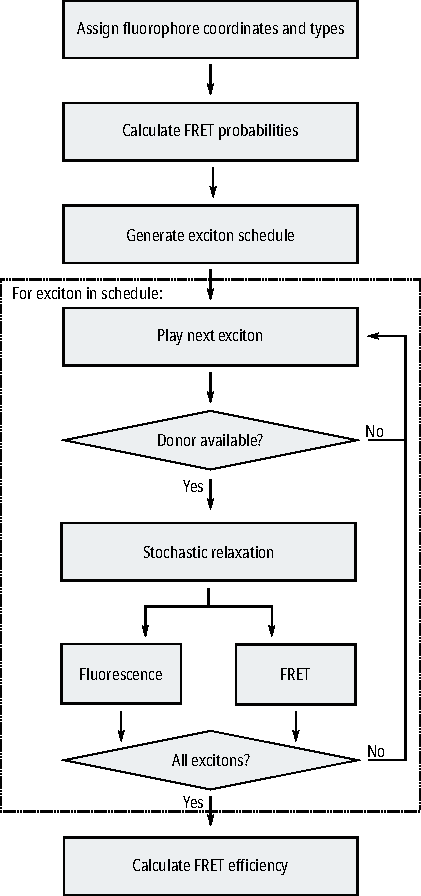
\includegraphics[width=\textwidth]{exifret_program.pdf}
	\end{subfigure}
	\end{minipage}
	\hfill
	\begin{minipage}{0.55\textwidth}
	\begin{subfigure}[t]{\textwidth}
		\caption{}\label{ch3fig:exifret_coords}
		\centering
		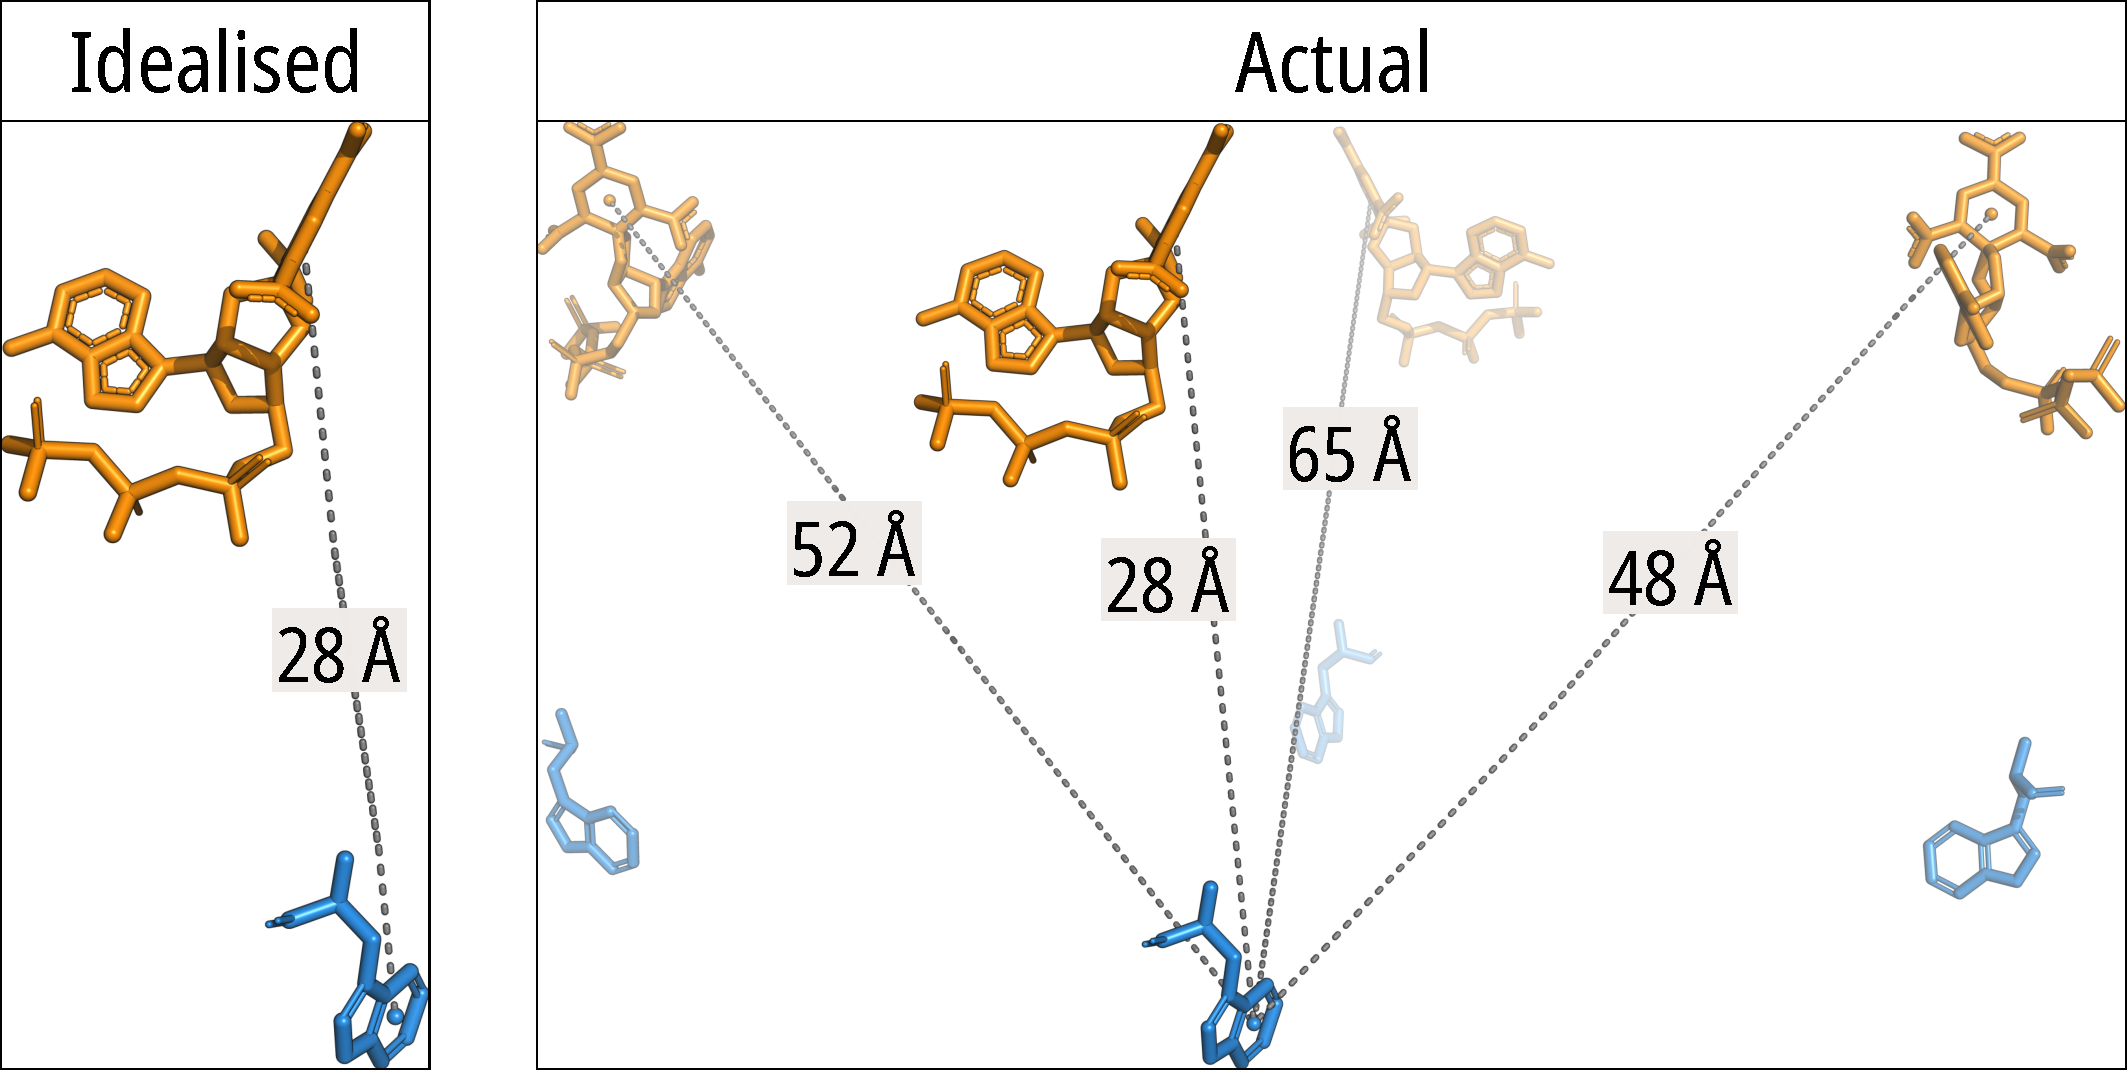
\includegraphics[width=\textwidth]{exifret_coords.pdf}
	\end{subfigure}
	\vfill
	\begin{subfigure}[t]{\textwidth}
		\caption{}\label{ch3fig:exifret_out}
		\centering
		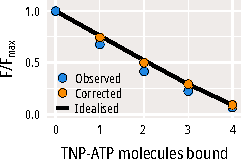
\includegraphics[width=\textwidth]{exifret_out.pdf}
	\end{subfigure}
	\end{minipage}
	\caption[Numerical analysis of FRET efficiency in tetrameric Kir6.2]{
	\subref{ch3fig:exifret_program} Schematic of the numerical simulation.
	After the geometry and fluorophore types are assigned, an exciton schedule is generated from the photon flux determined by the irradiance and wavelength of the LED used to excite ANAP.
	For each simulated photon (exciton), a relaxed donor is chosen at random.
	The donor releases its energy either via fluorescence or FRET to an acceptor based on the relative probability of each process.
	Donors and acceptors relax stochastically based on their fluorescence lifetimes (\SI{2}{\nano\second} for ANAP \cite{zagotta_measuring_2016-1} and \SI{0.05}{\nano\second} or \SI{2}{\nano\second} for TNP-ATP \cite{ye_spectroscopic_1999, ishikawa_single-molecule_2002}).
	Once the full exciton schedule is played, the total number of fluorescence and FRET events are summed and the total FRET efficiency is calculated.
	\subref{ch3fig:exifret_coords} Geometry of W311 and TNP-ATP molecules in tetrameric Kir6.2.
	W311 residues are from PDB \#6C3P, and TNP-ATP is from the highest scoring docking pose in Figure \ref{ch3fig:6c3p_docked}.
	Distances are measured from the centre of mass of the W311 sidechain to the centre of mass of each of the TNP moieties.
	\subref{ch3fig:exifret_out} Shown as a line is the idealised FRET efficiency for a single K\ATP{} channel bound to increasing numbers of TNP-ATP.
	Actual (blue) and corrected (orange) FRET efficiencies from the numerical simulation at each ligand occupancy state are shown as points.
	}
\end{figure}

Overall, these two corrections do not dramatically alter our results (Figure \ref{ch3fig:tnpatp_quenching_1}).
We observed quenching of ANAP fluorescence over a concentration range of TNP-ATP similar to the range in which we observed inhibition of current in W311*-GFP (Figure \ref{ch3fig:ec50_fits_3}, \ref{ch3fig:tnpatp_quenching_2}).
When fit to a Hill equation, quenching ($F/F_{max}$) was fit with an EC\textsubscript{50} of \SIrange{21}{31}{\micro\Molar}, while the corrected binding data (adjusted $F/F_{max}$) gave an EC\textsubscript{50} of \SIrange{30}{45}{\micro\Molar}.

\begin{figure}[h]
	\centering
	\begin{subfigure}[t]{0.45\textwidth}
		\caption{}\label{ch3fig:tnpatp_quenching_1}
		\centering
		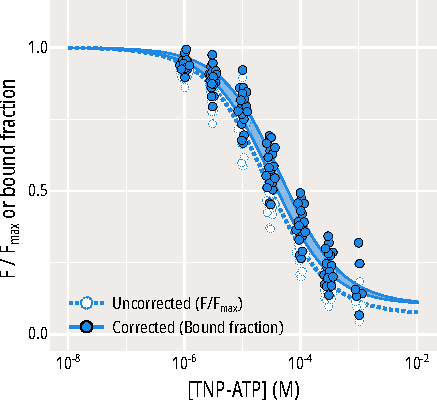
\includegraphics[width=\textwidth]{tnpatp_quenching_1.pdf}
	\end{subfigure}
	\hfill
	\begin{subfigure}[t]{0.45\textwidth}
		\caption{}\label{ch3fig:ec50_fits_3}
		\centering
		\includegraphics[width=\textwidth]{ec50_fits_3.pdf}
	\end{subfigure}
	\vfill
	\begin{subfigure}[t]{0.9\textwidth}
		\caption{}\label{ch3fig:tnpatp_quenching_2}
		\centering
		\includegraphics[width=\textwidth]{tnpatp_quenching_2.pdf}
	\end{subfigure}
	\caption[W311*-GFP unroofed membrane binding]{
	\subref{ch3fig:tnpatp_quenching_1} Fluorescence quenching of W311*-GFP+SUR1 by TNP-ATP in unroofed membrane patches.
	Each uncorrected point (white with dashed blue outline) represents an individual measurement normalised to the maximum current observed in that unroofed membrane.
	Each corrected point (blue filled points) has been transformed to $log_2(\frac{F}{F_{max}}+1)$.
	The smooth filled curves are the \SI{95}{\percent} intervals of the posterior probability distribution of fits to equation \ref{eq:hill} as described in the methods.
	The dashed curve is the median of the fits to the uncorrected data.
	\subref{ch3fig:ec50_fits_3} Posterior probability distribution for the population $EC_{50}$ values from fits to the corrected $F/F_{max}$ data.
	\subref{ch3fig:tnpatp_quenching_2} Data from each experiment is shown separately.
	The smooth filled curves are the \SI{95}{\percent} intervals of the posterior predictions for each experiment.
	}
\end{figure}

\subsection{Patch-clamp fluorometry of Kir6.2 constructs}

To ensure that the ANAP fluorescence we observe in the unroofed membranes is emitted by functional channels, we measured fluorescence quenching and current inhibition from the same excised patches (Figure \ref{ch3fig:atp_tnpatp_trace}, \ref{ch3fig:atp_tnpatp_spectra_1}, \ref{ch3fig:atp_tnpatp_spectra_2}).

This experimental paradigm leads to two complications compared to performing the measurements separately.
Firstly, the number of channels in an excised patch are far smaller than the number of channels in an unroofed membrane patch.
This results in a much dimmer fluorescence readout, and a lower signal-to-noise ratio.
Secondly, the presence of the pipette glass in the images results in some abnormalities in the background subtraction procedure.
This is not due to the glass itself, but results from the occlusion of TNP-ATP from the image surrounding the patch.
This leads to oversubtraction of the background TNP-ATP spectra, leading to an apparent negative peak in our corrected images.
However, we find that there is no overlap of this peak and the ANAP peak, so our fluorescence quenching measurements are unaffected by this phenomenon.
We were able to correct for ANAP bleaching in the same manner as we did for unroofed membranes (Figure \ref{ch3fig:pcf_bleaching}).

\begin{figure}[h]
	\centering
	\begin{subfigure}[t]{0.9\textwidth}
		\caption{}\label{ch3fig:bleaching_plots_1}
		\centering
		\includegraphics[width=\textwidth]{bleaching_plots_1.pdf}
	\end{subfigure}
	\vfill
	\begin{subfigure}[t]{0.45\textwidth}
		\caption{}\label{ch3fig:bleaching_terms_1}
		\centering
		\includegraphics[width=\textwidth]{bleaching_terms_1.pdf}
	\end{subfigure}
	\hfill
	\begin{subfigure}[t]{0.45\textwidth}
		\caption{}\label{ch3fig:bleaching_terms_2}
		\centering
		\includegraphics[width=\textwidth]{bleaching_terms_2.pdf}
	\end{subfigure}
	\caption[PCF bleaching correction]{
	\subref{ch3fig:bleaching_plots_1} Normalised ANAP fluorescence intensities in excised patches perfused at different concentrations of TNP-ATP are shown as points coloured according to the concentration of TNP-ATP.
	The black dashed lines are fits to the fluorescence intensities without TNP-ATP present with equation \ref{eq:bleaching}.
	\subref{ch3fig:bleaching_terms_1} Values of the two parameters in equation \ref{eq:bleaching} for fits to each of the experiments in \subref{ch3fig:bleaching_plots_2}.
	\subref{ch3fig:bleaching_terms_2} Proportion of ANAP fluorescence remaining unbleached in the last exposure taken without the presence of TNP-ATP in each experiment.
	The dashed line is the mean, with a value of $0.41$.
	}\label{ch3fig:pcf_bleaching}
\end{figure}

Our fluoresence measurements from excised patches are right-shifted when compared to our measurements for unroofed membranes (Figure \ref{ch3fig:pcf_1}), with an $EC_{50}$ value of \SIrange{76}{144}{\micro\Molar}.
Our finding that the EC\textsubscript{50} for TNP-ATP binding is right-shifted compared to the IC\textsubscript{50} for TNP-ATP inhibition is consistent between each experimental paradigm (Figure \ref{ch3fig:ec50_fits_4}).
This finding has implications for how exactly the binding of nucleotides to Kir6.2 leads to closure of the K\ATP{} channel pore.

\begin{figure}[h]
	\centering
	\begin{subfigure}[t]{0.9\textwidth}
		\caption{}\label{ch3fig:atp_tnpatp_trace}
		\centering
		\includegraphics[width=\textwidth]{atp_tnpatp_trace.pdf}
	\end{subfigure}
	\vfill
	\begin{subfigure}[t]{0.5\textwidth}
		\caption{}\label{ch3fig:atp_tnpatp_spectra_1}
		\centering
		\includegraphics[width=\textwidth]{atp_tnpatp_spectral_images.pdf}
	\end{subfigure}
	\hfill
	\begin{subfigure}[t]{0.4\textwidth}
		\caption{}\label{ch3fig:atp_tnpatp_spectra_2}
		\centering
		\includegraphics[width=\textwidth]{atp_tnpatp_spectral_traces.pdf}
	\end{subfigure}
	\vfill
	\begin{subfigure}[t]{0.45\textwidth}
		\caption{}\label{ch3fig:pcf_1}
		\centering
		\includegraphics[width=\textwidth]{pcf_1.pdf}
	\end{subfigure}
	\hfill
	\begin{subfigure}[t]{0.45\textwidth}
		\caption{}\label{ch3fig:ec50_fits_4}
		\centering
		\includegraphics[width=\textwidth]{ec50_fits_4.pdf}
	\end{subfigure}
	\caption[ANAP is not quenched by ATP]{
	\subref{ch3fig:atp_tnpatp_trace} Current trace from an excised patch expressing W311*-GFP+SUR1 perfused with either ATP or TNP-ATP.
	The zero current level is shown as a dotted line, and the nucleotide applications are marked as coloured bars.
	\subref{ch3fig:atp_tnpatp_spectra_1} Spectra captured from the same patch during the nucleotide applications marked in \subref{ch3fig:atp_tnpatp_trace}, and during the washout periods between applications.
	Each spectra was captured with a one second exposure and corrected for background fluorescence and bleaching as described elsewhere.
	\subref{ch3fig:atp_tnpatp_spectra_2} Averaged traces of the spectra shown in \subref{ch3fig:atp_tnpatp_spectra_1}. The location of the peak ANAP fluorescence is marked by a grey box.
	\subref{ch3fig:pcf_1} Current inhibition ($I/I_{max}$, orange points) and fluorescence quenching (Adjusted $F/F_{max}$, blue points) of W311*-GFP+SUR1 in excised membrane patches recorded simultaneously.
	The smooth filled curves are the \SI{95}{\percent} intervals of the posterior probability distribution of fits to equation \ref{eq:hill} as described in the methods.
	The dashed blue lines are the \SI{95}{\percent} intervals of the fits reported in Figure \ref{ch3fig:tnpatp_quenching_1}.
	\subref{ch3fig:ec50_fits_4} Posterior probability distributions for the estimated population $EC_{50}$ and $IC_{50}$ values are shown coloured according to their intervals.
	The dashed distribution is the posterior probability distribution reported in Figure \ref{ch3fig:ec50_fits_3}
	}
\end{figure}

\section{Discussion}

We have demonstrated that we can measure nucleotide binding to the inhibitory nucleotide binding site of Kir6.2 in intact, functional K\ATP{} channels in their native membrane environment.
Measuring binding directly in either unroofed membrane patches or in excised patches simultaneously with current recordings reveals that nucleotide binding is right-shifted compared to nucleotide inhibition; i.e. K\ATP{} channels begin to close at nucleotide concentrations where there is very little binding.
This observation rules out certain models of ion channel function, which will be explored further in chapter \ref{ch4}.

These findings come with some important caveats.
Firstly, the introduction of ANAP into Kir6.2 at residue 311 clearly impacts nucleotide inhibition of the channel, increasing the observed $IC_{50}$ values for ATP.
Our analysis of nucleotide binding and inhibition is therefore predicated on this decrease in sensitivity to ATP inhibition not reflecting a disruption of the normal physiological mechanism of ATP inhibition.
As all of our binding experiments are performed in the W311* background by necessity, we hope that measurements of relative changes in binding and inhibition will still be meaningfuly interpretable as they will mirror similar relative changes in inhibition observed in the WT background.

Secondly, K\ATP{} channels are more sensitive to inhibition by TNP-ATP than by ATP.
Again, this means that any conclusions we draw from experiments measuring relative changes in binding and inhibition rely on those relative changes affecting ATP binding and inhibition to a similar extent.
To try and ameliorate these caveats as best as we can, where possible we have performed control experiments in the WT background with ATP to ensure that introduced mutations result in similar relative effects on nucleotide inhibition despite the background of the construct or the identitity of the nucleotide.
As control experiments of this sort are not possible in unroofed membranes, where it is impossible to measure current inhibition, we have focused on patch-clamp fluorometry for constructs where expression is good enough to measure sufficient fluorescence.

This methodology should be readily adaptable to the study of other nucleotide-regulated channels, such as the P2X receptor family or CFTR.
\chapter{\label{ch:4}MWC modelling} 

\graphicspath{{figures/ch4/}}

\minitoc

\section{Modelling nucleotide regulation of the K\ATP{} channel}

The complex regulation of K\ATP{} channel activity by nucleotides and phosphoinositides has led to a wide range of scientists seeking to unify the constellation of structural and functional studies into one mechanistic framework, which is capable of explaining each aspect of channel regulation.
The importance of K\ATP{} channels in regulating insulin secretion, responding to cardiac stress, and protecting against seizures is one driving force behind the search for a model \cite{proks_modeling_2009}.
Another aim is more holistic; hoping that increasing our understanding of how the K\ATP{} channel is regulated by the interplay of its ligands may shed light on other ion channels or proteins \cite{garfinkel_modeling_2017}.
In any case, the primary goal of constructing a mathematical model of the K\ATP{} channel is to explain as much of the diversity of channel function as possible, while keeping the model as simple and biologically relevant as possible; a balancing act between completeness and complexity.

Previous attempts at modelling K\ATP{} channel regulation have primarily focused on nucleotide inhibition \cite{trapp_molecular_1998, enkvetchakul_kinetic_2000, markworth_atp4-_2000, ribalet_regulation_2000, enkvetchakul_atp_2001-1, drain_concerted_2004, proks_gating_2005, li_ligand-dependent_2005, ribalet_atp-sensitive_2006-1, craig_how_2008-1}, due to the relative ease of isolating the effects of nucleotide inhibition.
There have been fewer attempts at incorporating activation by Mg-nucleotides \cite{ribalet_regulation_2000, proks_activation_2010-1, vedovato_nucleotide-binding_2015}.
The difficulty in quantifying phosphinositide regulation of the K\ATP{} channel means that in most cases where it is considered, it is implicitly included as an effect on nucleotide sensitivity, rather than explicitly described \cite{baukrowitz_pip2_1998, fan_phosphoinositides_1999, enkvetchakul_kinetic_2000}, although there are some exceptions \cite{ribalet_regulation_2000, enkvetchakul_atp_2001-1}.

\subsection{Restricting the subset of possible models}


\subsection{Determining open probability}
Noise analysis - you can get a correct answer the wrong way (Puljung).

Measuring the open probability of an ion channel is most accurately accomplished by single-channel electrophysiological recordings, which allows direct measurement of the time a channel spends in an open state.
This approach does not allow for the determination of the open probability of a population of channels great than 2/3 at a time, as it becomes increasingly difficult to separate the openings of different channels in the population.
Thus it would not be possible to determine single channel open probability simultaneously with nucleotide binding, as the fluorescence signal from a small number of channels would be impossible to resolve.

Another approach is noise analysis of currents from large populations of channels.
The 'noise' in noise analysis refers to current fluctuations which occur when recording from a population of ion channels due to the stochastic channel gating of individual channels.
If there are a constant number of channels ($N$) which are gated independently from each other and share a homogenous open probability ($P_O$) and a single open conductance level ($i$), the observed macroscopic current level $I$ can be described by equation \ref{eq:inpo}:
\begin{equation}\label{eq:inpo}
	I = iNP_O
\end{equation}
and the observed variance of the macroscopic current can be described by the variance of the binomial distribution, equation \ref{eq:bin_1}:
\begin{equation}\label{eq:bin_1}
	\sigma^2 = NP_O \cdot (1 - P_O) \cdot i^2
\end{equation}
where the single channel current is essentially a scaling factor.
If we assume that in a given recording $N$ and $i$ remain constant, and it is $P_O$ which changes in response to any given stimuli, then we can combine equations \ref{eq:inpo} and \ref{eq:bin_1} to yield equation \ref{eq:bin_2}:
\begin{equation}\label{eq:bin_2}
	\sigma^2 = iI - \frac{1}{N} \cdot I^2
\end{equation}
This equation yields a parabola from $I = 0$ to $I = Ni$.
Intuitively, there can be no variance when $P_O$ is exactly 0 or 1, as there will be no opening or closing events which can give rise to current fluctuations.
Once $i$ and $N$ have been determined for a given experiment, the observed current magnitude $I$ can be converted into the $P_O$ for the population of channels by rearranging equation \ref{eq:inpo} as follows:
\begin{equation}\label{eq:poin}
	P_O = \frac{I}{iN}
\end{equation}

Equation \ref{eq:bin_2} can be fit to experimental data by calculating the variance of observed current at different current magnitudes.
This calculation is not exactly trivial, and has been accomplished a number of different ways for different purposes.
For channels with fast inactivation such as the Na\textsubscript{V} family, non-stationary noise analysis involves repeating a stimulus multiple times and measuring variance as the squared sum of deviations from the mean of the current magnitude calculated at the same time point across multiple stimuli, referred to in the literature as an 'isochrone'.
For channels which do not inactivate, stationary noise analysis is possible, and variance can be measured as the squared sum of deviations from the mean current magnitude over a period of time for which $I$ is 'stationary'(Figure \ref{ch4fig:noise_example_1}, \ref{ch4fig:noise_example_2}, \ref{ch4fig:noise_example_3}).

Stationary noise analysis has been described for K\ATP{} channels before by a number of different researchers (Shyng, Paolo, Peter).
Unfortunately, in most of the published research the exact procedure for extracting the parameters in equation \ref{eq:bin_1} is described in the methods section, but the quality of the fits and the value of the fitted parameters besides the final calculated $P_O$ is not discussed.
A notable exception to this rule is (Paolo), in which two findings are discussed.
Firstly, fitting equation \ref{eq:bin_2} to the mean and variance of \SI{200}{\milli\second} sections of macroscopic currents from wild-type Kir6.2+SUR2A resulted in a systematic underestimation of the single channel current $i$.
From single channel experiments, the single channel current was determined to be \SI{4}{\pico\ampere}, while the value obtained from fitting macroscopic currents was only \SI{2}{\pico\ampere}.
In the case of WT-GFP+SUR1, we see a similar understimation of single channel current (Figure \ref{ch4fig:noise_example_fits_1}, \ref{ch4fig:noise_example_fits_2}, \ref{ch4fig:noise_example_fits_3}), with fits yielding estimates of \SIrange{1.66}{2.64}{\pico\ampere}, while measured single channel currents are at least \SI{4}{\pico\ampere}.
This underestimate of $i$ is most likely due to an underestimate of channel current variance as $P_O$ increases, which could be due to two main reasons.

Firstly, the process of filtering and digitising channel currents can lead to underestimates of variance depending on the relationship between the open time of the measured channel and the cut-off frequency of the filter used.
It is unlikely that this phenomenon is responsible for our findings, as the K\ATP{} mean open time duration is close to \SI{1}{\milli\second} and filtering at \SI{5}{\kilo\hertz} would lead to less than a \SI{5}{\percent} underestimation of $i$.
Even if the mean open time of WT-GFP+SUR1 was closer to \SI{0.1}{\milli\second}, we would expect a \SI{20}{\percent} reduction rather than the \SI{50}{\percent} we actually observe.
Empirically, we can use the frequency power spectrum of our measured current fluctuations to determine whether there may be high frequency channel openings we are missing (Figure \ref{ch4fig:spectra_converge}).
For WT-GFP+SUR1, we observe that at frequencies approaching our filter cut-off at \SI{5}{\kilo\hertz} there is very little observed amplitude in active channels when compared to fully inhibited channels, suggesting we are not missing high frequency current fluctuations.

\begin{figure}[h]
	\centering
	\begin{subfigure}[t]{0.3\textwidth}
		\caption{}\label{ch4fig:noise_example_1}
		\centering
		\includegraphics[width=\textwidth]{noise_example_1.pdf}
	\end{subfigure}
	\hfill
	\begin{subfigure}[t]{0.3\textwidth}
		\caption{}\label{ch4fig:noise_example_2}
		\centering
		\includegraphics[width=\textwidth]{noise_example_2.pdf}
	\end{subfigure}
	\hfill
	\begin{subfigure}[t]{0.3\textwidth}
		\caption{}\label{ch4fig:noise_example_3}
		\centering
		\includegraphics[width=\textwidth]{noise_example_3.pdf}
	\end{subfigure}
	\vfill
	\begin{subfigure}[t]{0.3\textwidth}
		\caption{}\label{ch4fig:noise_example_fits_1}
		\centering
		\includegraphics[width=\textwidth]{noise_example_fits_1.pdf}
	\end{subfigure}
	\hfill
	\begin{subfigure}[t]{0.3\textwidth}
		\caption{}\label{ch4fig:noise_example_fits_2}
		\centering
		\includegraphics[width=\textwidth]{noise_example_fits_2.pdf}
	\end{subfigure}
	\hfill
	\begin{subfigure}[t]{0.3\textwidth}
		\caption{}\label{ch4fig:noise_example_fits_3}
		\centering
		\includegraphics[width=\textwidth]{noise_example_fits_3.pdf}
	\end{subfigure}
	\vfill
	\begin{subfigure}[t]{0.5\textwidth}
		\caption{}\label{ch4fig:spectra_converge}
		\centering
		\includegraphics[width=\textwidth]{spectra_converge.pdf}
	\end{subfigure}
	\caption[Systematic underestimation of single channel currents]{
	\subref{ch4fig:noise_example_1},\subref{ch4fig:noise_example_2},\subref{ch4fig:noise_example_3} 5 second extracts from three separate recordings of WT-GFP+SUR1 currents.
	Extracts from different recordings are coloured differently.
	The zero current level determined by barium is indicated as a dashed line.
	\subref{ch4fig:noise_example_fits_1}, \subref{ch4fig:noise_example_fits_2}, \subref{ch4fig:noise_example_fits_3} Plots of the mean current and variance for each of the extracts in the panel above.
	Fits to equation x are shown as a solid line when $i$ is allowed to vary freely, and as a dashed line when $i$ is fixed to \SI{4.32}{\pico\ampere}.
	The fitted value for $i$ is shown for each recording separately.
	\subref{ch4fig:spectra_converge} Averaged power spectra for the three recordings analysed.
	The blue line is the power spectra when channels are fully inhibited and represents the background, while the orange line is the power spectra when channels are most active.
	The high frequency components of the current fluctuations are attenuated to near background levels above \SIrange{2}{3}{\kilo\hertz}.
	}\label{ch4fig:noise_manual}
\end{figure}

Secondly, an underestimation of $i$ could occur due to violations in the underlying assumptions of the binomial distribution.
The first two assumptions are that $N$ and $i$ are constant throughout a recording.
We know that $i$ does not change on nucleotide inhibition of K\ATP{} channels, noris it affected by PIP\textsubscript{2} and rundown.
Additionally, in excised patches it is improbable that there will be any change in $N$ during the course of a recording.
The third assumption is that the channels in a patch share a homogenous $P_O$, which exhibits graded changes in response to stimuli (in our case, application of nucleotide).
This assumption is far harder to justify for our experimental condition, in which channel rundown due to loss of PIP\textsubscript{2} results in a complicated mixture of channel populations with different $P_O$s.

An extreme case in which channels transition between two states, one where $0 < P_O < 1$ and one where $P_O \approx 0$ can be approximated by equation \ref{eq:bin_1}, with a channel transitioning to the $P_O \approx 0$ state essentially considered to be no longer available to open, thus reducing $N$.
Thus, fitting the observed current-variance data with \ref{eq:bin_1} would yield a straight line where the slope of the line is equal to $i \cdot (1 - P_O)$.
This formulation of equation \ref{eq:bin_1} has been used successfully in the analysis of currents from CRAC channels, VSOA channels, and in the analysis of a specific cardiac K\ATP{} channel mutation.
Unfortunately, in our case channel rundown does not render the K\ATP{} channel completely unable to open, with fully rundown channels displaying single channel open probabilities in the range of \numrange{0.05}{0.25}.
Instead of each current measurement being a draw from a single binomial distribution, we are instead drawing from a mixture of binomial distributions with different $P_O$s.
We can demonstrate how this leads to an underestimation of $i$ by simulating a simple case where there are two populations of channels, $a$ and $b$, one with a tenfold lower $P_O$ than the other.

\begin{equation}\label{eq:bibi_sim}
\begin{split}
	N_a + N_b &= 1000 \\
	0 < P_{O_{a}} &< 1 \\
	P_{O_{b}} &= \frac{P_{O_{a}}}{10}
\end{split}
\end{equation}

\begin{figure}[h]
	\centering
	\begin{subfigure}[t]{0.3\textwidth}
		\caption{}\label{ch4fig:simulated_noise_1}
		\centering
		\includegraphics[width=\textwidth]{simulated_noise_1.pdf}
	\end{subfigure}
	\hfill
	\begin{subfigure}[t]{0.3\textwidth}
		\caption{}\label{ch4fig:simulated_noise_2}
		\centering
		\includegraphics[width=\textwidth]{simulated_noise_2.pdf}
	\end{subfigure}
	\hfill
	\begin{subfigure}[t]{0.3\textwidth}
		\caption{}\label{ch4fig:simulated_noise_3}
		\centering
		\includegraphics[width=\textwidth]{simulated_noise_3.pdf}
	\end{subfigure}
	\caption[Simulated multibinomial currents]{
	}\label{ch4fig:noise_sim}
\end{figure}

\begin{figure}[h]
	\centering
	\begin{subfigure}[t]{0.9\textwidth}
		\caption{}\label{ch4fig:noise_fits_1}
		\centering
		\includegraphics[width=\textwidth]{noise_fits_1.pdf}
	\end{subfigure}
	\vfill
	\begin{subfigure}[t]{0.9\textwidth}
		\caption{}\label{ch4fig:noise_fits_2}
		\centering
		\includegraphics[width=\textwidth]{noise_fits_2.pdf}
	\end{subfigure}
	\caption[Estimating open probability from stationary noise analysis]{
	\subref{ch4fig:noise_fits_1} Plots of the mean current and variance for 1 second extracts from recordings of WT-GFP+SUR1 (blue) or W311*-GFP+SUR1 (orange).
	Fits to equation x are shown as a solid line when $i$ is allowed to vary freely, and as a dashed line when $i$ is fixed to \SI{4.32}{\pico\ampere}.
	The straight, finer dashed lines are fits to equation y only using the linear portion of the data, which are shown as solid filled points outlined in black.
	\subref{ch4fig:noise_fits_2} Parameter estimates from fits in \subref{ch4fig:noise_fits_1} are shown as separate points for each experiment.
	For fits to equation x, open probability is calculated from the intial current on patch excision.
	To visualise the spread, normal distributions are plotted alongside the point estimates, limited to $0 < x < 1$.
	}\label{ch4fig:all_noise_fits}
\end{figure}

\section{Implementing an MWC model}

\subsection{A simple case}

The simplest case of an allosteric MWC model for an ion channel is shown as Scheme I in Figure \ref{ch4fig:mwc_model_diagrams}.
This simple case assumes a channel composed of a single monomer with a single binding site for ligand $A$.
The channel is restricted to two states, open and closed.
These two states exist in an equilibrium described by L, which is equivalent to $\frac{[open]}{[closed]}$.
Ligand $A$ binds to the protein with a microscopic affinity constant $K_A$.
The ligand $A$ differentially stabilises the open and closed states by a constant $D$.
When $D$ is unity, the ligand $A$ binds equally to both states and so does not influence the conformational changes of the channel.
When $D>1$, the ligand $A$ preferentially stabilises the open state, while when $D<1$ the ligand instead preferentially stabilises the closed state.

\begin{figure}[h]
	\centering
	\begin{subfigure}[t]{0.9\textwidth}
		\caption{}\label{ch4fig:mwc_model_diagrams}
		\centering
		\includegraphics[width=\textwidth]{mwc_model_diagrams.pdf}
	\end{subfigure}
	\vfill
	\begin{subfigure}[t]{0.3\textwidth}
		\caption{}\label{ch4fig:mwc_scheme_1_fits}
		\centering
		\includegraphics[width=\textwidth]{mwc_scheme_1_fits.pdf}
	\end{subfigure}
	\hfill
	\begin{subfigure}[t]{0.3\textwidth}
		\caption{}\label{ch4fig:mwc_scheme_2_fits}
		\centering
		\includegraphics[width=\textwidth]{mwc_scheme_2_fits.pdf}
	\end{subfigure}
	\hfill
	\begin{subfigure}[t]{0.3\textwidth}
		\caption{}\label{ch4fig:mwc_scheme_3_fits}
		\centering
		\includegraphics[width=\textwidth]{mwc_scheme_3_fits.pdf}
	\end{subfigure}
	\vfill
	\begin{subfigure}[t]{0.9\textwidth}
		\caption{}\label{ch4fig:mwc_params_1}
		\centering
		\includegraphics[width=\textwidth]{mwc_scheme_param_fits.pdf}
	\end{subfigure}
	\caption[Generating data from MWC model schemes]{
	\subref{ch4fig:mwc_model_diagrams} Equilibrium diagrams for the three MWC schemes considered.
	For each scheme, only the parameters newly relevant for that scheme are shown explicitly.
	\subref{ch4fig:mwc_scheme_1_fits}, \subref{ch4fig:mwc_scheme_2_fits}, \subref{ch4fig:mwc_scheme_3_fits} Data generated from Scheme I (\subref{ch4fig:mwc_scheme_1_fits}), Scheme II (\subref{ch4fig:mwc_scheme_2_fits}) or Scheme III (\subref{ch4fig:mwc_scheme_3_fits}) all fit to Scheme I.
	The input parameters are shown above each panel.
	$L$ differs between \subref{ch4fig:mwc_scheme_1_fits} and \subref{ch4fig:mwc_scheme_2_fits}, \subref{ch4fig:mwc_scheme_3_fits} due to the introduction of a resting PIP\textsubscript{2} concentration, which in Scheme I is implicitly incorporated into $L$.
	\subref{ch4fig:mwc_params_1} Parameter estimates for the Scheme I model fit to the data generated by all three schemes.
	The input parameter value is marked as a black vertical line for each panel.
	}\label{ch4fig:mwc_models}
\end{figure}

\subsection{The role of PIP\textsubscript{2}}

If we consider introducing a second ligand B which binds to a distinct site on the same monomer and does not directly interact with ligand A, we introduce the states shown in Scheme II of Figure \ref{ch4fig:mwc_model_diagrams}.
Each ligand has its own microscopic association constant ($K_A$ or $K_B$) and its own preference for the open or closed states ($D_A$ or $D_B$).
Importantly, there is no interaction term between ligand $A$ and ligand $B$; the only way the binding of the ligands can impact each other is through effects on $L$.
Scheme II is therefore a restricted form of scheme III, which explicity introduces a term for local interaction ($C$) between binding sites for ligands $A$ and $B$ on the same monomer.
When $C$ is unity, Scheme III becomes Scheme II.
When $C<1$, binding of one ligand reduces the ability of the other ligand to bind on the same monomer.
When $C>1$, binding of one ligand enhances the ability of the other ligand to bind on the same monomer.

To study nucleotide binding to Kir6.2, I have used Scheme I (expanded to incorporate four identical monomers) as an approximation of the K\ATP{} channel, with ligand $A$ representing nucleotides.
To determine whether this approximation is appropriate, I generated data using each of the three schemes as the underlying model of channel function and then fit the generated observations to Scheme I (Figure \ref{ch4fig:mwc_scheme_1_fits}, \ref{ch4fig:mwc_scheme_2_fits}, \ref{ch4fig:mwc_scheme_3_fits}).
Ten individual sets of observations were generated using the inputs shown above each figure panel as the centre of a lognormal distribution with a standard deviation of 0.25.
These observations were then fit to Scheme I (as done previously throughout the thesis) and the values of the three free parameters ($K_A$, $D_A$ and $L$) were estimated (Figure \ref{ch4fig:mwc_params_1}).

\begin{figure}[h]
	\centering
	\begin{subfigure}[t]{0.3\textwidth}
		\caption{}\label{ch4fig:scheme_1_ka_shift}
		\centering
		\includegraphics[width=\textwidth]{mwc_scheme_1_ka_shift.pdf}
	\end{subfigure}
	\hfill
	\begin{subfigure}[t]{0.3\textwidth}
		\caption{}\label{ch4fig:scheme_1_da_shift}
		\centering
		\includegraphics[width=\textwidth]{mwc_scheme_1_da_shift.pdf}
	\end{subfigure}
	\hfill
	\begin{subfigure}[t]{0.3\textwidth}
		\caption{}\label{ch4fig:scheme_1_l_shift}
		\centering
		\includegraphics[width=\textwidth]{mwc_scheme_1_l_shift.pdf}
	\end{subfigure}
	\vfill
	\begin{subfigure}[t]{0.9\textwidth}
		\caption{}\label{ch4fig:mwc_params_2}
		\centering
		\includegraphics[width=\textwidth]{mwc_scheme_param_fits_2.pdf}
	\end{subfigure}
	\caption[Parameter retrieval from MWC models]{
	\subref{ch4fig:scheme_1_ka_shift}, \subref{ch4fig:scheme_1_da_shift}, \subref{ch4fig:scheme_1_l_shift} Data generated from Scheme I with \subref{ch4fig:scheme_1_ka_shift} $K_A$ shifted from $10^4$ to $10^3$, \subref{ch4fig:scheme_1_da_shift} $D_A$ shifted from $0.1$ to $0.8$, or \subref{ch4fig:scheme_1_l_shift} $L$ shifted from $1$ to $10$.
	\subref{ch4fig:mwc_params_} Parameter estimates from each of the model fits.
	In each case, the modified parameter is retrieved accurately and no other parameters are affected.
	}\label{ch4fig:scheme_1_shifts}
\end{figure}

We know that Scheme I is only an approximation of nucleotide binding as it does not explicitly include PIP\textsubscript{2}.
The question is, if the underlying data generating model is Scheme II which explicitly includes a second ligand, are we still able to extract meaningful parameter estimates by fitting the observed data to Scheme I?
In addition,to date it remains unclear whether there is local allostery between the nucleotide and PIP\textsubscript{2} binding sites.
The existence of local allostery would mean that Scheme III, which includes an explicit term for this interaction, would best represent the true data generating model.
We can show that even when Scheme II or Scheme III are the underlying data generating model, with ligand $B$ representing PIP\textsubscript{2}, we are still able to extract the true values of $K_A$ and $D_A$ by fitting the generated data to Scheme I (Figure \ref{ch4fig:mwc_models}).
Parameter choices for Scheme II and III are such that the open probability of the channel at 0 [ATP] is still 50\%, equivalent to $L=1$ in Scheme I.
I really need to redo this with the true $L$ set to $0.01$ instead of $0.1$ as that is closer to post rundown open proability...

We can also show that when Scheme I is the underlying data generating model, changes in any of the three parameters are easily identified and retrieved by fitting the observed data to Scheme I (Figure \ref{ch4fig:scheme_1_shifts}).
This suggests that introducing mutations which directly effect any of the three parameters of this model would be easily identifiable if Scheme I was the true underlying model.

What if Scheme II or III were the underlying model?
We would still expect changes in the three parameters which exist in Scheme I to be identifiable (I should probably check this), although $L$ would not represent the true unliganded open/closed equilibrium as we would be estimating an $L$ modified by the resting PIP\textsubscript{2} concentration, $K_B$, $D_B$ and $C$ - in this case, the estimated $L$ parameter in fact represents the ATP-unbound open/closed equilibrium.

\begin{figure}[h]
	\centering
	\begin{subfigure}[t]{0.45\textwidth}
		\caption{}\label{ch4fig:scheme_2_kb_shift}
		\centering
		\includegraphics[width=\textwidth]{mwc_scheme_2_kb_shift.pdf}
	\end{subfigure}
	\hfill
	\begin{subfigure}[t]{0.45\textwidth}
		\caption{}\label{ch4fig:scheme_3_kb_shift}
		\centering
		\includegraphics[width=\textwidth]{mwc_scheme_3_kb_shift.pdf}
	\end{subfigure}
	\vfill
	\begin{subfigure}[t]{0.9\textwidth}
		\caption{}\label{ch4fig:mwc_params_3}
		\centering
		\includegraphics[width=\textwidth]{mwc_scheme_param_fits_3.pdf}
	\end{subfigure}
	\caption[Parameter retrieval from MWC models]{
	\subref{ch4fig:scheme_2_kb_shift}, \subref{ch4fig:scheme_3_kb_shift} Data generated from \subref{ch4fig:scheme_2_kb_shift} Scheme II  or \subref{ch4fig:scheme_3_kb_shift} with $K_B$ shifted from $10^5$ to $10^6$.
	}\label{ch4fig:scheme_2_3_shifts}
\end{figure}

However, it is unclear how changes in parameters which are not explicitly modelled in Scheme I will affect the generated data and the parameter estimates obtained by fitting the data to Scheme I.
Figure \ref{ch4fig:scheme_2_3_shifts} shows the results of increasing $K_B$ by tenfold on data generated from Scheme II (Figure \ref{ch4fig:scheme_2_kb_shift}) or Scheme III (Figure \ref{ch4fig:scheme_3_kb_shift}).
The first observation of note is that the generated data closely resemble those generated from Scheme I when $L$ is increased (Figure \ref{ch4fig:scheme_1_l_shift}), and indeed when the $L$ parameter estimates for a tenfold shift in $K_B$ in Scheme II/III and tenfold shift in $L$ for Scheme I are compared (Figure \ref{ch4fig:mwc_params_3}, right panel) are compared they appear to be similar.
So far so good, as an observed increase in $L$ when fit with Scheme I would lead us to draw the correct inferences about changes in the underlying model (i.e. the open probability of the cnall has indeed increased).
However, changes in $K_B$ are not perfectly captured by changes in $L$ when fit to scheme I.
Notably, if local allostery exists between the nucleotide and PIP\textsubscript{2} binding site - if Scheme III is the true underlying model - then fitting the observed data to Scheme I would lead us to estimate an incorrect value for $K_A$ (Figure \ref{ch4fig:scheme_2_kb_shift}).
Thus, if there is local allostery between the sites, then a mutation which induces an increase in the binding affinity for PIP\textsubscript{2} would not just increase our estimate of $L$ (which would lead to a correct inference) but it would also decrease our estimate of $K_A$ by a not-insignificant amount, which could lead to the incorrect inference that a mutation is causing a direct change in nucleotide binding when it is in fact causing a direct change in PIP\textsubscript{2} binding, which through local allostery is influencing our estimates of $K_A$.

\chapter{\label{ch:5}Nucleotide regulation of Kir6.2} 

\graphicspath{{figures/ch5/}}

\minitoc

\section{Introduction}

There are variety of ways in which mutations in Kir6.2 can lead to altered K\ATP{} channel function, and often lead to diseases of insulin secretion \cite{ashcroft_katp_2013, aguilar-bryan_neonatal_2008, hattersley_activating_2005, ashcroft_neonatal_2017, flanagan_update_2009, ashcroft_diabetes_2012, pipatpolkai_new_2020-1}.
These can be divided into two broad categories; mutations which have a ligand-independent effect, and those which affect the ligand-dependent regulation of the channel, covered in more detail in Chapter \ref{ch1-intro}.
Nucleotide inhibition of the K\ATP{} channel can be altered by mutations through three separate mechanistic routes.
A mutation which reduces sensitivity of the channel to nucleotide inhibition may act by either reducing the affinity of binding of nucleotides to Kir6.2, increasing the open probability of the channel, reducing the transduction of nucleotide binding to channel closure, or a combinatuon of all three.

Interrogation of residues in this second category is very difficult using electrophysiological measures alone, as without measuring binding of nucleotides directly it is hard to truly separate effects on open probability from effects on binding and transduction \cite{colquhoun_binding_1998}.
In this chapter, we aim to clarify the role of several residues implicated in regulating the inhibitory effect of nucleotides on K\ATP{} channel function by measuring TNP-ATP binding directly to the inhibitory nucleotide binding site on Kir6.2, where possible in conjunction with simultaneous current measurements.

\section{Nucleotide binding}

\subsection{G334D abolishes nucleotide binding}

Residue G334 of Kir6.2 is located in the C-terminal region (Figure \ref{ch5fig:g334d_loc}) and has been hypothesised to form part of the ATP binding site since electrophysiological studies demonstrated a dramatic reduction in nucleotide sensitivity upon mutation of the residue \cite{drain_katp_1998, li_open_2002, li_ligand-dependent_2005}.
In addition, mutation of this residue to aspartic acid (G334D) results in severe permanent neonatal diabetes mellitus \cite{masia_atp-binding_2007-1}.
This hypothesis was confirmed by the solving of cryo-EM structures of K\ATP{} in the presence of ATP, which revealed the close proximity of residue G334 to the bound ATP \cite{lee_molecular_2017, martin_anti-diabetic_2017, li_structure_2017, puljung_cryo-electron_2018-1}.
Mutating G334 to a total of 13 different amino acid substitutions led to a increase in the IC\textsubscript{50} for ATP by over an order of magnitude in excised patches \cite{li_ligand-dependent_2005}.
However, only two of those substitutions (R and K) resulted in any changes in nucleotide-independent channel gating when examined at the single-channel level, with unliganded $P_O$ remaining constant.
It has therefore been suggested that while G334 forms part of the ATP binding site of Kir6.2, it does not participate in channel gating or transduction of ligand binding to the channel pore.

\begin{figure}[h]
	\centering
	\begin{subfigure}[t]{0.45\textwidth}
		\caption{}\label{ch5fig:g334d_loc}
		\centering
		\includegraphics[width=\textwidth]{g334d_1.pdf}
	\end{subfigure}
	\hfill
	\begin{subfigure}[t]{0.45\textwidth}
		\caption{}\label{ch5fig:g334d_popfits}
		\centering
		\includegraphics[width=\textwidth]{g334d_2.pdf}
	\end{subfigure}
	\vfill
	\begin{subfigure}[t]{0.9\textwidth}
		\caption{}\label{ch5fig:g334d_indfits}
		\centering
		\includegraphics[width=\textwidth]{g334d_3.pdf}
	\end{subfigure}
	\vfill
	\begin{subfigure}[t]{0.7\textwidth}
		\caption{}\label{ch5fig:g334d_params}
		\centering
		\includegraphics[width=\textwidth]{g334d_4.pdf}
	\end{subfigure}
	\caption[G334D abolishes nucleotide binding at Kir6.2]{
	\subref{ch5fig:g334d_loc} Residue G334 is shown in purple in the cryo-EM structure of K\ATP{} (PDB \#6C3P).
	Adjacent subunits of Kir6.2 are shown in two different shades of yellow, TMD0 and L0 of SUR1 are shown in two different shades of blue.
	The core of SUR1 is not shown.
	Bound ATP is shown in red.
	\subref{ch5fig:g334d_popfits} Fluorescence quenching of W311*,G334D-GFP+SUR1 by TNP-ATP in unroofed membrane patches.
	Each point represents an individual experiment.
	The smooth filled curves are the \SI{95}{\percent} intervals of the posterior probability distribution of fits to equation \ref{eq:hill} as described in the methods.
	\subref{ch5fig:g334d_indfits} Data from each experiment is shown separately.
	The smooth filled curves are the \SI{95}{\percent} intervals of the posterior predictions for each experiment.
	\subref{ch5fig:g334d_params} Posterior probability distributions for the estimated population $EC_{50}$ values are shown coloured according to their intervals.
	}\label{ch5fig:g334d}
\end{figure}

We sought to test this directly by measuring the binding of TNP-ATP in unroofed membranes to W311*,G334D-GFP+SUR1.
Fluorescence spectra captured from unroofed membrane patches expressing W311*,G334D-GFP+SUR1 were indistinguishable from those expressing W311*-GFP+SUR1.
The location of the ANAP peak and the bleaching characteristics were also identical.
We found that ANAP fluorescence from W311*,G334D-GFP+SUR1 was barely quenched by even \SI{1}{\milli\Molar} TNP-ATP (Figure \ref{ch5fig:g334d_popfits}, \ref{ch5fig:g334d_indfits}), reducing the apparant binding EC\textsubscript{50} from \SIrange{30}{45}{\micro\Molar} to at least \SI{2.8}{\milli\Molar} (Figure \ref{ch5fig:g334d_params}).
We cannot be sure of the upper bound of the apparent binding EC\textsubscript{50} given how little quenching we were able to achieve even with \SI{1}{\milli\Molar} TNP-ATP.
Unfortunately, we were unable to resolve macroscopic currents from W311*,G334D-GFP+SUR1 in excised patches despite seeing fluorescence in unroofed membranes.
Thus, we were unable to measure nucleotide inhibition of this construct ourselves.
In electrophysiological experiments on K\ATP{} channels containing the G334D mutation, other studies have found that currents are insensitive to inhibition by ATP even up to \SI{10}{\Molar} \cite{drain_katp_1998, masia_atp-binding_2007-1}.
In the framework of our MWC model, the only explanation for a dramatic decrease in both nucleotide binding and inhibition is a decrease in $K_A$, the microscopic binding affinity.
However, as we were unable to measure TNP-ATP inhibition ourselves, we were unable to determine whether the G334D substitution affected transduction in addition to this binding effect.

\section{Channel gating}

\subsection{C166S alters inhibition without affecting binding}

Residue C166 of Kir6.2 is located at the cytosolic end of the second transmembrane domain (Figure \ref{ch5fig:c166s_loc}, \cite{lee_molecular_2017, martin_anti-diabetic_2017, li_structure_2017, puljung_cryo-electron_2018-1}), and has been suggested to play a role in regulating the intrinsic gating of the channel \cite{gloyn_kcnj11_2006, trapp_molecular_1998, ribalet_atp-sensitive_2006, yang_palmitoylation_2020, loussouarn_structure_2000, enkvetchakul_kinetic_2000}.
Mutations at this residue lead to dramatically increased unliganded $P_O$ in single-channel experiments \cite{trapp_molecular_1998, enkvetchakul_kinetic_2000, ribalet_atp-sensitive_2006}, and a reduction in sensitivity to nucleotide inhibition at both single-channel and the macroscopic level \cite{trapp_molecular_1998, enkvetchakul_kinetic_2000, ribalet_atp-sensitive_2006, li_decomposition_2013, yang_palmitoylation_2020}.
In addition, two substitutions at this residue (F and Y) have been found to cause severe neonatal diabetes \cite{gloyn_kcnj11_2006}.
Electrophysiological measurements alone are not sufficient to distinguish between the reduction in sensitivity to nucleotide inhibition being caused by the increase in intrinsic $P_O$ alone, or whether there is an additional disregulation of transduction.

We measured TNP-ATP binding to W311*,C166S-GFP+SUR1 in unroofed membranes to determine the how mutations at C166 reduce sensitivity to nucleotide inhibition (Figure \ref{ch5fig:c166s_unroofed}).
We observed no real change in binding of TNP-ATP to the channel, with an EC\textsubscript{50} of \SIrange{44}{74}{\micro\Molar}.
If the C166S mutation solely increases the $P_O$ of the channel, we would expect an increase in the apparent EC\textsubscript{50} of nucleotide binding due to the preference of nucleotides for the closed state of the channel.
This finding therefore suggests a role for C166 in the transduction of nucleotide binding to the channel pore.

\begin{figure}[h]
	\centering
	\begin{subfigure}[t]{0.45\textwidth}
		\caption{}\label{ch5fig:c166s_loc}
		\centering
		\includegraphics[width=\textwidth]{c166s_1.pdf}
	\end{subfigure}
	\hfill
	\begin{subfigure}[t]{0.45\textwidth}
		\caption{}\label{ch5fig:c166s_popfits}
		\centering
		\includegraphics[width=\textwidth]{c166s_2.pdf}
	\end{subfigure}
	\vfill
	\begin{subfigure}[t]{0.9\textwidth}
		\caption{}\label{ch5fig:c166s_indfits}
		\centering
		\includegraphics[width=\textwidth]{c166s_3.pdf}
	\end{subfigure}
	\vfill
	\begin{subfigure}[t]{0.7\textwidth}
		\caption{}\label{ch5fig:c166s_params}
		\centering
		\includegraphics[width=\textwidth]{c166s_4.pdf}
	\end{subfigure}
	\caption[C166S does not alter nucleotide binding]{
	\subref{ch5fig:c166s_loc} Residue C166 is shown in purple in the cryo-EM structure of K\ATP{} (PDB \#6C3P).
	Adjacent subunits of Kir6.2 are shown in two different shades of yellow, TMD0 and L0 of SUR1 are shown in two different shades of blue.
	The core of SUR1 is not shown.
	Bound ATP is shown in red.
	\subref{ch5fig:c166s_popfits} Fluorescence quenching of W311*,C166S-GFP+SUR1 by TNP-ATP in unroofed membrane patches.
	Each point represents an individual experiment.
	The smooth filled curves are the \SI{95}{\percent} intervals of the posterior probability distribution of fits to equation \ref{eq:hill} as described in the methods.
	\subref{ch5fig:c166s_indfits} Data from each experiment is shown separately.
	The smooth filled curves are the \SI{95}{\percent} intervals of the posterior predictions for each experiment.
	\subref{ch5fig:c166s_params} Posterior probability distributions for the estimated population $EC_{50}$ values are shown coloured according to their intervals.
	}\label{ch5fig:c166s_1}
\end{figure}

To investigate this further, we excised patches expressing W311*,C166S-GFP+SUR1 and measured current inhibition and fluorescence quenching by TNP-ATP simultaneously (Figure \ref{ch5fig:c166s_traces}).
We found that the apprent affinity for nucleotide binding was indistinguishable from that for W311*-GFP+SUR1, and similar to our observations in unroofed membranes (Figure \ref{ch5fig:c166s_popfits_2}, EC\textsubscript{50} of \SIrange{26}{218}{\micro\Molar}).
Consistent with the literature, we did observe a large reduction in the apparent sensitivity of W311*,C166S-GFP+SUR1 currents to inhibition by TNP-ATP (Figure \ref{ch5fig:c166s_popfits_3}, IC\textsubscript{50} of at least \SI{155}{\micro\Molar}).
Intuitively, a change in nucleotide-dependent channel gating which is not accompanied by a change in nucleotide binding must be due (at least in part) to a change in the transduction of nucleotide binding to channel gating.

\begin{figure}[h]
	\centering
	\begin{subfigure}[t]{0.6\textwidth}
		\caption{}\label{ch5fig:c166s_traces}
		\centering
		\includegraphics[width=\textwidth]{c166s_5.pdf}
	\end{subfigure}
	\hfill
	\begin{subfigure}[t]{0.3\textwidth}
		\caption{}\label{ch5fig:c166s_popfits_2}
		\centering
		\includegraphics[width=\textwidth]{c166s_6.pdf}
	\end{subfigure}
	\vfill
	\begin{subfigure}[t]{0.3\textwidth}
		\caption{}\label{ch5fig:c166s_popfits_3}
		\centering
		\includegraphics[width=\textwidth]{c166s_7.pdf}
	\end{subfigure}
	\hfill
	\begin{subfigure}[t]{0.6\textwidth}
		\caption{}\label{ch5fig:c166s_params_2}
		\centering
		\includegraphics[width=\textwidth]{c166s_8.pdf}
	\end{subfigure}
	\vfill
	\begin{subfigure}[t]{0.9\textwidth}
		\caption{}\label{ch5fig:c166s_indfits_2}
		\centering
		\includegraphics[width=\textwidth]{c166s_9.pdf}
	\end{subfigure}
	\caption[C166S alters sensitivity to nucleotide inhibition]{
	\subref{ch5fig:c166s_traces} Current inhibition (left) and fluorescence quenching (right) from an excised patch expressing W311*,C166S-GFP+SUR1.
	The concentration of TNP-ATP perfused is shown by colour.
	The location of the peak ANAP fluorescence is marked as a grey box.
	\subref{ch5fig:c166s_popfits_2} Fluorescence quenching of W311*,C166S-GFP+SUR1 by TNP-ATP in excised patches.
	Each point represents an individual experiment.
	The smooth filled curves are the \SI{95}{\percent} intervals of the posterior probability distribution of fits to equation \ref{eq:hill} as described in the methods.
	\subref{ch5fig:c166s_popfits_3} Current inhibition of W311*,C166S-GFP+SUR1 by TNP-ATP in excised patches.
	Each point represents an individual experiment.
	The smooth filled curves are the \SI{95}{\percent} intervals of the posterior probability distribution of fits to equation \ref{eq:hill} as described in the methods.
	\subref{ch5fig:c166s_params_2} Posterior probability distributions for the estimated population EC\textsubscript{50} (blue) and IC\textsubscript{50} (orange) values are shown shaded according to their intervals.
	\subref{ch5fig:c166s_indfits_2} Data from each experiment is shown separately; each column represents one excised patch..
	The smooth filled curves are the \SI{95}{\percent} intervals of the posterior predictions for each experiment.
	}\label{ch5fig:c166s_2}
\end{figure}

Fitting our data to the MWC-type model described previously (Figure \ref{ch5fig:c166s_mwc_fit_1}, \ref{ch5fig:c166s_mwc_fit_2}), we found that in addition to the effects of the C166S mutation on the intrinsic open probability of K\ATP{}, there is a striking shift in $D_A$ (Figure \ref{ch5fig:c166s_mwc_params_1}).
This shift to a value much closer to unity indicates that binding of TNP-ATP to W311*,C166S-GFP+SUR1 favours the closed state far less than binding of TNP-ATP to W311*-GFP+SUR1.
Equivalently, binding of TNP-ATP to the mutant channel is less able to induce closure of the pore.
Thus, even at millimolar concentrations of TNP-ATP when all of the Kir6.2 subunits are predicted to be bound by nucleotide, the mutant K\ATP{} channels are still able to open.

\begin{figure}[h]
	\centering
	\begin{subfigure}[t]{0.45\textwidth}
		\caption{}\label{ch5fig:c166s_mwc_fit_1}
		\centering
		\includegraphics[width=\textwidth]{mwc_c166s_1.pdf}
	\end{subfigure}
	\hfill
	\begin{subfigure}[t]{0.45\textwidth}
		\caption{}\label{ch5fig:c166s_mwc_fit_2}
		\centering
		\includegraphics[width=\textwidth]{mwc_c166s_3.pdf}
	\end{subfigure}
	\vfill
	\begin{subfigure}[t]{0.9\textwidth}
		\caption{}\label{ch5fig:c166s_mwc_params_1}
		\centering
		\includegraphics[width=\textwidth]{mwc_c166s_2.pdf}
	\end{subfigure}
	\caption[C166S alters transduction of nucleotide binding to Kir6.2]{
	\subref{ch5fig:c166s_mwc_fit_1}, \subref{ch5fig:c166s_mwc_fit_2} Nucleotide binding (\subref{ch5fig:c166s_mwc_fit_1}) and current inhibition (\subref{ch5fig:c166s_mwc_fit_2}) of W311*,C166S-GFP+SUR1 by TNP-ATP in excised patches, data the same as in Figure \subref{ch5fig:c166s_popfits_2}, \subref{ch5fig:c166s_popfits_3}.
	The solid lines are the \SI{95}{\percent} intervals of the posterior probability distribution of fits to the MWC model paramaterised in equations \ref{eq:mwc_binding} and \ref{eq:normalised_po}.
	The dotted lines are the equivalent intervals for MWC fits to the W311*-GFP+SUR1 construct as shown in Figure \ref{ch3fig:pcf_1}.
	White circles are the inhibition of current by \SI{10}{\milli\Molar} ATP in separate experiments.
	\subref{ch5fig:c166s_mwc_params_1} Posterior probability distributions for the estimated population $L$, $D_A$ and $K_A$ values are shown shaded according to their intervals.
	}\label{ch5fig:c166s_3}
\end{figure}

Notably, the MWC fit to the current inhibition data has wide \SI{95}{\percent} posterior probability intervals (Figure \ref{ch5fig:c166s_mwc_fit_2}).
Unfortunately, we were not able to use higher concentrations of TNP-ATP due to its purification as a TEA\textsuperscript{+} salt.
High \si{\milli\Molar} concentrations of TEA\textsuperscript{+} inhibit K\ATP{} channels, and we determined that for W311*-GFP+SUR1 and W311*,C166S-GFP+SUR1 concentrations of above \SI{1}{\milli\Molar} TEA\textsuperscript{+} began to inhibit currents to an extent that would interfere with our measurements (Figure \ref{ch5fig:tea_trace}, \ref{ch5fig:tea_drc}).
The precise ratio of TEA\textsuperscript{+} to TNP-ATP in our solutions is unknown, but is assumed to be between 1:1 and 3:1.
Any additional inhibition observed at TNP-ATP concentrations greater than \SI{1}{\milli\Molar} for W311*,C166S-GFP+SUR1 will therefore be (at least in part) due to the presence of TEA\textsuperscript{+}.
However, we do see that even at concentrations of \SI{10}{\milli\Molar} ATP, W311*,C166S-GFP+SUR1 is not fully inhibited (Figure \ref{ch5fig:c166s_mwc_fit_2}, open circle).

Curiously, despite the wide posterior probability intervals for the MWC fit to the observed current inhibiton data in Figure \ref{ch5fig:c166s_mwc_fit_2}, the probability distributions for the underlying parameter values for W311*,C166S-GFP+SUR1 are not much wider than those observed for W311*-GFP+SUR1 (Figure \ref{ch5fig:c166s_mwc_params_1}).
Thus, the variability of current inhibition observed for \SI{1}{\milli\Molar} TNP-ATP is not due to increased uncertainty in our MWC parameter estimates.
Instead, the variability may reflect that the C166S substitution alters the nucleotide regulation of the K\ATP{} channel such that small changes in the energetics of the underlying gating mechanism result in large changes in the observed current.
This may help to explain the differences in inhibition of K\ATP{} channels with substitutions at C166 by high nucleotide concentrations observed across multiple electrophysiological studies \cite{trapp_mechanism_1998, enkvetchakul_atp_2001-1, ribalet_atp-sensitive_2006-1, yang_palmitoylation_2020}.

\begin{figure}[h]
	\centering
	\begin{subfigure}[t]{0.45\textwidth}
		\caption{}\label{ch5fig:tea_trace}
		\centering
		\includegraphics[width=\textwidth]{tea_trace.pdf}
	\end{subfigure}
	\hfill
	\begin{subfigure}[t]{0.45\textwidth}
		\caption{}\label{ch5fig:tea_drc}
		\centering
		\includegraphics[width=\textwidth]{tea_drc.pdf}
	\end{subfigure}
	\caption[TEA\textsubscript{+} inhibits K\ATP{} channels at high concentrations]{
	\subref{ch5fig:tea_trace} Representative current trace from an excised patch expressing W311*,C166S-GFP+SUR1.
	Applications of different concentrations of TEA\textsubscript{+} are indicated by bars shaded red, and application of \SI{10}{\milli\Molar} ATP is indicated in black.
	The zero-current level is marked with a dotted line.
	\subref{ch5fig:tea_drc} Concentration-response data for W311*-GFP+SUR1 (blue) and W311*,C166S-GFP+SUR1 (green) current inhibition by TEA\textsubscript{+}.
	The lines are fits to equation \ref{eq:hill} with $I_{max}$ fixed to 0.
	}\label{ch5fig:c166s_4}
\end{figure}

\subsection{Mutations at E179 alter both inhibition and binding}

Residue E179 of Kir6.2 is located in the C-terminal region of Kir6.2 between the inhibitory nucleotide binding site and the proposed PIP\textsubscript{2} binding site.
In one early predicted structures of Kir6.2, it was theorised that E179 would form part of the nucleotide binding pocket directly, potentially coordinating the adenine ring of ATP directly through hydrogen bonding \cite{antcliff_functional_2005}.
In another, it was hypothesised to form part of the PIP\textsubscript{2} binding pocket instead \cite{haider_identification_2007}.
Electrophysiological experiments painted a confusing picture of the residues role \cite{antcliff_functional_2005}.
Mutation to an amino acid capable of forming hydrogen bonds (Q) resulted in no change in the IC\textsubscript{50} for nucleotide inhibition (although a separate study found that Q increased the IC\textsubscript{50} \cite{proks_involvement_1999}), while only one of two amino acids incapable of forming hydrogen bonds tested (M and L) resulted in an increased IC\textsubscript{50}.
In addition, mutation of the residue to asparagine (which is not capable of forming hydrogen bonds) not only dramatically increased the nucleotide IC\textsubscript{50}, but increased the intrinsic open probability of the channel \cite{antcliff_functional_2005}.

\begin{figure}[h]
	\centering
	\begin{subfigure}[t]{0.45\textwidth}
		\caption{}\label{ch5fig:e179_loc}
		\centering
		\includegraphics[width=\textwidth]{e179_1.pdf}
	\end{subfigure}
	\hfill
	\begin{subfigure}[t]{0.45\textwidth}
		\caption{}\label{ch5fig:e179_atp_popfits}
		\centering
		\includegraphics[width=\textwidth]{e179_2.pdf}
	\end{subfigure}
	\vfill
	\begin{subfigure}[t]{0.45\textwidth}
		\caption{}\label{ch5fig:e179_tnpatp_popfits_1}
		\centering
		\includegraphics[width=\textwidth]{e179_3.pdf}
	\end{subfigure}
	\hfill
	\begin{subfigure}[t]{0.45\textwidth}
		\caption{}\label{ch5fig:e179_tnpatp_popfits_2}
		\centering
		\includegraphics[width=\textwidth]{e179_4.pdf}
	\end{subfigure}
	\caption[Functional effects of E179 mutations]{
	\subref{ch5fig:e179_loc} Residue E179 is shown in purple in the cryo-EM structure of K\ATP{} (PDB \#6C3P).
	Adjacent subunits of Kir6.2 are shown in two different shades of yellow, TMD0 and L0 of SUR1 are shown in two different shades of blue.
	The core of SUR1 is not shown.
	Bound ATP is shown in red.
	\subref{ch5fig:e179_atp_popfits}, \subref{ch5fig:e179_tnpatp_popfits_1} Current inhibition of E179 mutants in the WT-GFP+SUR1 and W311*-GFP+SUR1 background by ATP (\subref{ch5fig:e179_atp_popfits}) or TNP-ATP (\subref{ch5fig:e179_tnpatp_popfits_1}).
	Each point represents an individual experiment.
	The smooth filled curves are the \SI{95}{\percent} intervals of the posterior probability distribution of fits to equation \ref{eq:hill} as described in the methods.
	\subref{ch5fig:e179_tnpatp_popfits_2} Fluorescence quenching of E179 mutants in the W311*-GFP+SUR1 background by TNP-ATP acquired simultaneously with the inhibition data in panel \subref{ch5fig:e179_tnpatp_popfits_1}.
	Each point represents an individual experiment.
	The smooth filled curves are the \SI{95}{\percent} intervals of the posterior probability distribution of fits to equation \ref{eq:hill} as described in the methods.
	\subref{ch5fig:e179_ec50_fits} Posterior probability distributions for the estimated population $IC_{50}$ or $EC_{50}$ values are shown in purple ($IC_{50}$ for ATP inhibition), orange ($IC_{50}$ for TNP-ATP inhibition), or blue ($EC_{50}$ for TNP-ATP binding).
	Each distribution is shaded with respect to its intervals.
	}\label{ch5fig:e179_1}
\end{figure}

\begin{figure}[h]
	\centering
	\begin{subfigure}[t]{0.9\textwidth}
		\caption{}\label{ch5fig:e179_ec50_fits}
		\centering
		\includegraphics[width=\textwidth]{e179_5.pdf}
	\end{subfigure}
	\caption[E179 mutations $EC_{50}$ parameters]{
	\subref{ch5fig:e179_ec50_fits} Posterior probability distributions for the estimated population $IC_{50}$ or $EC_{50}$ values are shown in purple ($IC_{50}$ for ATP inhibition), orange ($IC_{50}$ for TNP-ATP inhibition), or blue ($EC_{50}$ for TNP-ATP binding).
	Each distribution is shaded with respect to its intervals.
	}\label{ch5fig:e179_1a}
\end{figure}

The cryo-EM structures of K\ATP{} in complex with ATP revealed that bound ATP adopted a radically different conformation to that proposed in early models, and the E179 side chain actually lies over \SI{8}{\angstrom} away from bound ATP \cite{lee_molecular_2017, martin_anti-diabetic_2017, li_structure_2017, puljung_cryo-electron_2018-1} (FIgure \ref{ch5fig:e179_loc}.
Unfortunately, no structure has been resolved in the presence of PIP\textsubscript{2} to date.
However, coarse-grained molecular dynamics simulations using the cryo-EM structures as a starting point indicate that E179 may form part of the PIP\textsubscript{2} binding pocket \cite{pipatpolkai_evaluating_2020}.
In addition, mutation to E179K results in reduced inhibition of the channel by the sequestering agent neomycin - potentially due to an increased affinity of the mutated residue for PIP\textsubscript{2} \cite{pipatpolkai_evaluating_2020}.

To attempt to resolve the precise role of E179 in nucleotide binding and inhibition, we first determined how ATP and TNP-ATP inhibiton of K\ATP{} channels was affected by mutation of E179 to A or K (Figure \ref{ch5fig:e179_atp_popfits}, \ref{ch5fig:e179_tnpatp_popfits_1}.
For E179A-GFP+SUR1 and E179K-GFP+SUR1, we observed an increase in IC\textsubscript{50} for both ATP and TNP-ATP inhibition (Figure \ref{ch5fig:e179_ec50_fits}).
ATP inhibition did not seem to be influenced by the identity of the replacement amino acid (\SIrange{49}{145}{\micro\Molar} and \SIrange{43}{138}{\micro\Molar} respectively), while TNP-ATP inhibition was less reduced by mutation to an A than a K (\SIrange{6.5}{21}{\micro\Molar} and \SIrange{16}{87}{\micro\Molar} respectively).
Introducing the mutations into the ANAP-labelled construct did not affect the relative changes in inhibition by either nucleotide, with ATP inhibition occurring at similar IC\textsubscript{50}s for A and K (\SIrange{162}{562}{\micro\Molar} and \SIrange{191}{479}{\micro\Molar} respectively) and with A increasing the IC\textsubscript{50} for TNP-ATP less than K (\SIrange{14}{44}{\micro\Molar} and \SIrange{42}{224}{\micro\Molar} respectively).
Measurements of TNP-ATP binding mirrored our observations for current inhibition by TNP-ATP, with mutation to both A and K resulting in an increased apparant binding EC\textsubscript{50}, with A having less of an effect than K (\SIrange{166}{417}{\micro\Molar} and \SIrange{347}{813}{\micro\Molar} respectively).
Fitting the combined data to the MWC-type model, we found that both mutations resulted in a decreased $K_A$ estimate, with no apparent change in $L$.
In addition, mutation to a K led to a $D_A$ value closer to unity than for E or the wild-type A (Figure \ref{ch5fig:e179_2}).

\begin{figure}[h]
	\centering
	\begin{subfigure}[t]{0.9\textwidth}
		\caption{}\label{ch5fig:mwc_e179_1}
		\centering
		\includegraphics[width=\textwidth]{mwc_e179_1.pdf}
	\end{subfigure}
	\vfill
	\begin{subfigure}[t]{0.9\textwidth}
		\caption{}\label{ch5fig:mwc_e179_2}
		\centering
		\includegraphics[width=\textwidth]{mwc_e179_2.pdf}
	\end{subfigure}
	\caption[E179 mutations affect gating and nucleotide binding]{
	\subref{ch5fig:mwc_e179_1} Current inhibition (orange) and fluorescence quenching (blue) from excised patches expressing W311*,E179A-GFP+SUR1 (left) or W311*,E179K-GFP+SUR1 (right).
	The smooth filled curves are the \SI{95}{\percent} intervals of the posterior probability distribution of fits to equations \ref{eq:mwc_binding} and \ref{eq:normalised_po}.
	Dashed curves are for comparison, and indicate the \SI{95}{\percent} intervals of the posterior probability distribution of fits to equations \ref{eq:mwc_binding} and \ref{eq:normalised_po} for the W311*-GFP+SUR1 data.
	\subref{ch5fig:mwc_e179_2} Posterior probability distributions for the estimated population $L$, $D$ and $K_A$ parameters from the fits in panel \subref{ch5fig:mwc_e179_1}.
	Each distribution is shaded with respect to its intervals.
	}\label{ch5fig:e179_2}
\end{figure}

\subsection{Mutations at K39 alter both inhibition and binding}

Residue K39 of Kir6.2 is located in the N-terminal region of Kir6.2, and is positioned between the inhibitory nucleotide binding site and the proposed PIP\textsubscript{2} binding site (Figure \ref{ch5fig:k39_loc}).
In previous studies, the mutation K39A has shown a small reduction in open probability \cite{cukras_role_2002}, and a small reduction in sensitivity to nucleotide inhibition \cite{cukras_role_2002, tucker_molecular_1998}.
These effects are somewhat contradictory, as mutations which reduce open probability tend also to increase sensitivity to nucleotide inhibition.
In each of the cryo-EM structures of K\ATP{}, the K39 side chain appears to coordinate the bound ATP molecule \cite{lee_molecular_2017, martin_anti-diabetic_2017, li_structure_2017, puljung_cryo-electron_2018-1}.
These structures are presumed to represent the closed state of the channel, and no PIP\textsubscript{2} bound structure of the channel has yet been solved.
However, molecular dynamics simulations using the ATP-bound structure as a starting point and introducing PIP\textsubscript{2} suggest that the K39 residue is able to contact both ligands (in press).
This suggests a potential role for K39 in the binding sites of both ATP and PIP\textsubscript{2}, which may explain the contradictory findings of open probability and nucleotide inhibition changes when the residue is mutated.

\begin{figure}[h]
	\centering
	\begin{subfigure}[t]{0.45\textwidth}
		\caption{}\label{ch5fig:k39_loc}
		\centering
		\includegraphics[width=\textwidth]{k39_1.pdf}
	\end{subfigure}
	\hfill
	\begin{subfigure}[t]{0.45\textwidth}
		\caption{}\label{ch5fig:k39_atp_popfits}
		\centering
		\includegraphics[width=\textwidth]{k39_2.pdf}
	\end{subfigure}
	\vfill
	\begin{subfigure}[t]{0.45\textwidth}
		\caption{}\label{ch5fig:k39_tnpatp_popfits_1}
		\centering
		\includegraphics[width=\textwidth]{k39_3.pdf}
	\end{subfigure}
	\hfill
	\begin{subfigure}[t]{0.45\textwidth}
		\caption{}\label{ch5fig:k39_tnpatp_popfits_2}
		\centering
		\includegraphics[width=\textwidth]{k39_4.pdf}
	\end{subfigure}
	\caption[Functional effects of K39 mutations]{
	\subref{ch5fig:k39_loc} Residue K39 is shown in purple in the cryo-EM structure of K\ATP{} (PDB \#6C3P).
	Adjacent subunits of Kir6.2 are shown in two different shades of yellow, TMD0 and L0 of SUR1 are shown in two different shades of blue.
	The core of SUR1 is not shown.
	Bound ATP is shown in red.
	\subref{ch5fig:k39_atp_popfits}, \subref{ch5fig:k39_tnpatp_popfits_1} Current inhibition of K39 mutants in the WT-GFP+SUR1 and W311*-GFP+SUR1 background by ATP (\subref{ch5fig:k39_atp_popfits}) or TNP-ATP (\subref{ch5fig:k39_tnpatp_popfits_1}).
	Each point represents an individual experiment.
	The smooth filled curves are the \SI{95}{\percent} intervals of the posterior probability distribution of fits to equation \ref{eq:hill} as described in the methods.
	\subref{ch5fig:k39_tnpatp_popfits_2} Fluorescence quenching of K39 mutants in the W311*-GFP+SUR1 background by TNP-ATP acquired simultaneously with the inhibition data in panel \subref{ch5fig:k39_tnpatp_popfits_1}.
	Each point represents an individual experiment.
	The smooth filled curves are the \SI{95}{\percent} intervals of the posterior probability distribution of fits to equation \ref{eq:hill} as described in the methods.
	}\label{ch5fig:k39_1}
\end{figure}

\begin{figure}[h]
	\centering
	\begin{subfigure}[t]{0.9\textwidth}
		\caption{}\label{ch5fig:k39_ec50_fits}
		\centering
		\includegraphics[width=\textwidth]{k39_5.pdf}
	\end{subfigure}
	\caption[K39 mutations $EC_{50}$ parameters]{
	\subref{ch5fig:k39_ec50_fits} Posterior probability distributions for the estimated population $IC_{50}$ or $EC_{50}$ values are shown in purple ($IC_{50}$ for ATP inhibition), orange ($IC_{50}$ for TNP-ATP inhibition), or blue ($EC_{50}$ for TNP-ATP binding).
	Each distribution is shaded with respect to its intervals.
	}\label{ch5fig:k39_1a}
\end{figure}

We tested three mutations at K39 (K39A, K39E, K39R) to examine the effects of changing the side chain characteristics on nucleotide binding and inhibition.
Mutation to E (opposite charge) or R (same charge) results in an increase in IC\textsubscript{50} for ATP inhibition for both WT and W311* backgrounds (Figure \ref{ch5fig:k39_atp_popfits}, \ref{ch5fig:k39_ec50_fits}).
We did not see an increase in the IC\textsubscript{50} for ATP inhibition when K39 was mutated to A (neutral) in either background (Figure \ref{ch5fig:k39_atp_popfits}, \ref{ch5fig:k39_ec50_fits}).
Inhibition by TNP-ATP displayed a different profile depending on the mutant residue (Figure \ref{ch5fig:k39_tnpatp_popfits_1}).
In both WT and W311* backgrounds, inhibition by TNP-ATP exhibited higher IC\textsubscript{50} values for K39A and K39E than we observed for K39R, which was not really distinguishable from K39 (\ref{ch5fig:k39_ec50_fits}).
Our docked conformation for TNP-ATP suggests that the TNP-moiety of the nucleotide may result in extra contacts with K39 compared to ATP, which may be the cause of the different sensitivity to inhibition between the two nucleotides when this residue is mutated.
Measurements of TNP-ATP binding showed increases in the EC\textsubscript{50} estimates for each of the three mutations (Figure \ref{ch5fig:k39_tnpatp_popfits_2}, \ref{ch5fig:k39_ec50_fits}).

Fits of the combined data to the MWC model gave parameter estimates for $K_A$ that decreased from K>R>E>A (Figure \ref{ch5fig:k39_2}).
In addition, mutation to an E or an A resulted in $D_A$ values closer to unity.
Interpretation of these parameters for the R and A mutations is frustrated by the differences in inhibition between TNP-ATP and ATP; we cannot be sure that these differences in binding and inhibition are due to the identity of the nucleotide rather than the identity of the residue.
However, the K39E mutation displayed similar inhibition for both TNP-ATP and ATP.
The increase in our estimate for $D_A$ when K39 is mutated to an A or an E, but not for R, may indicate a positive charge at the sidechain of this residue being important for transduction of nucleotide binding to the channel pore.

\begin{figure}[h]
	\centering
	\begin{subfigure}[t]{0.9\textwidth}
		\caption{}\label{ch5fig:mwc_k39_1}
		\centering
		\includegraphics[width=\textwidth]{mwc_k39_1.pdf}
	\end{subfigure}
	\vfill
	\begin{subfigure}[t]{0.9\textwidth}
		\caption{}\label{ch5fig:mwc_k39_2}
		\centering
		\includegraphics[width=\textwidth]{mwc_k39_2.pdf}
	\end{subfigure}
	\caption[K39 mutations affect gating and nucleotide binding]{
	\subref{ch5fig:mwc_k39_1} Current inhibition (orange) and fluorescence quenching (blue) from excised patches expressing W311*,K39A-GFP+SUR1 (left), W311*,K39E-GFP+SUR1 (middle), or W311*,K39R-GFP+SUR1 (right).
	The smooth filled curves are the \SI{95}{\percent} intervals of the posterior probability distribution of fits to equations \ref{eq:mwc_binding} and \ref{eq:normalised_po}.
	Dashed curves are for comparison, and indicate the \SI{95}{\percent} intervals of the posterior probability distribution of fits to equations \ref{eq:mwc_binding} and \ref{eq:normalised_po} for the W311*-GFP+SUR1 data.
	\subref{ch5fig:mwc_k39_2} Posterior probability distributions for the estimated population $L$, $D$ and $K_A$ parameters from the fits in panel \subref{ch5fig:mwc_k39_1}.
	Each distribution is shaded with respect to its intervals.
	}\label{ch5fig:k39_2}
\end{figure}

\section{Discussion}

Fitting a concerted MWC model to the combined datasets obtained by measuring TNP-ATP binding to Kir6.2 in combination with current inhibition allows us to distinguish between mutations which affect nucleotide binding, ligand-independent channel gating, and transduction of nucleotide binding to channel gating.
This is best demonstrated by our results for W311*,C166S-GFP+SUR1, which we propose not only increases the unliganded $P_O$ of the K\ATP{} channel as described many times previously (illustrated in this experiment by the increase in $L$ from the MWC fit), but also reduces the ability of TNP-ATP to induce channel closure ($D_A$ approaches unity).
Substitutions of C166 must therefore alter the structure of the channel such that in addition to the unliganded open state being more energetically favourable than in wild-type channels, nucleotides are no longer able to stabilise the closed state to the same extent as in wild type channels.

We can quantify this difference by calculating the energy contribution of nucleotide binding to the closed state of the two constructs at saturating concentrations of TNP-ATP, given by the formula $-RTln({D_A}^4)$ where $R$ is the gas constant and $T$ is the absolute temperature (assumed to be \SI{296}{\kelvin}).
The free energy TNP-ATP binding contributes to the closed state of W311*-GFP+SUR1 is \SIrange{23.0}{63.4}{\kilo\joule\per\Molar}, while the free energy TNP-ATP binding contributes to the closed state of W311*,C166S-GFP+SUR1 is only \SIrange{20.4}{-3.05}{\kilo\joule\per\Molar}.
However, as the transduction of binding is a combination of both the channel and the ligand, it is possible that TNP-ATP stabilises the closed state of the channel to a different extent than ATP.

Interpretation of our findings for substitutions at E179 and K39 of Kir6.2 are not as straightforward.
Mutations at these residues lead to a complex mixture of changes to both the microscopic binding affinity for TNP-ATP ($K_A$) and the transduction of nucleotide binding ($D_A$).
Given that E179 is predicted to form part of the PIP\textsubscript{2} binding site \cite{haider_identification_2007, pipatpolkai_evaluating_2020}, we might expect mutations at this location to alter the $P_O$ of channels in excised patches due to changes in the PIP\textsubscript{2} binding affinity.
\citeauthor{antcliff_functional_2005} found that mutation to asparagine increased the $P_O$ of K\ATP{} channels in excised patches, while \citeauthor{pipatpolkai_evaluating_2020} observed that mutation to a lysine caused a reduction in the IC\textsubscript{50} for neomycin inhibition of the channel.
Here, mutation to alanine or lysine did not result in a change in our estimate for $L$, which we would expect to see if there was a change in the $P_O$ of the channel resulting from altered OIP\textsubscript{2} affinity.
Instead, we observed changes in our estimates for $K_A$, the microscopic binding affinity for TNP-ATP, and $D_A$, the transduction of nucleotide binding to channel gating.

We believe there are two possible ways to interpret these findings.
The first is to accept the shift in $K_A$ at face value - a decrease in the apparent TNP-ATP binding affinity would suggest a role for residue E179 in forming the nucleotide binding pocket, and this function is abrogated by our mutations.
Despite the distance of the residue from the bound ATP, there could be interactions between E179 and the sidechains of residues which do form the pocket (e.g. R54), such that mutation of E179 leads to alterations in the binding pocket which reduce nucleotide binding affinity and therefore our estimate of $K_A$.
The additional effect on $D_A$ caused by mutating the residue to K suggests a dysregulation of the transduction of nucleotide binding to the channel pore, making nucleotides less selective for the closed state.

The second interpretation is possible due to the simplification of the role of PIP\textsubscript{2} in our MWC model as discussed in chapter \ref{ch:4}.
Briefly, if there is an additional allosteric interaction between nucleotide and PIP\textsubscript{2} binding to Kir6.2 which is separate to the channels open/closed state, then changes in $K_A$ may reflect alterations in the affinity for PIP\textsubscript{2} binding in addition to or instead of alterations in the affinity for nucleotide binding.
Thus, the decrease in $K_A$ upon mutation of E179 may reflect an increase in PIP\textsubscript{2} affinity and demonstrate the presence of local allostery between nucleotide and lipid.

Distinguishing between these two interpretations is difficult given our current evidence, and essentially depends on the weight you place on the assumptions of each, but should be possible with one or two further experiments.
Firstly, an increase in PIP\textsubscript{2} affinity should lead to an increase in channel open probability on excision (barring an effect on the relative preference of PIP\textsubscript{2} for the open state).
Our inability to accurately determine the open probability of the macroscopic experiments described so far could be supplemented by single channel analysis of the mutants to test this directly.
In addition, we could measure the affinity of PIP\textsubscript{2} directly in macroscopic patches.
Finally, to definitively test the existence of local allostery between the nucleotide and PIP\textsubscript{2} binding sites, we could introduce PIP\textsubscript{2} binding mutants into the C166S background.
C166S channels exhibit almost no nucleotide-dependent gating; i.e. nucleotide binding is uncoupled from gating of the channel pore.
Thus, any changes observed in nucleotide binding in the C166S background when PIP\textsubscript{2} affinity is changed would have to be due to a local allosteric interaction which does not involve the pore.

\begin{figure}[h]
	\centering
	\begin{subfigure}[t]{0.45\textwidth}
		\caption{}\label{ch5fig:k39_clash_atp}
		\centering
		\includegraphics[width=\textwidth]{k39_clash_atp.pdf}
	\end{subfigure}
	\hfill
	\begin{subfigure}[t]{0.45\textwidth}
		\caption{}\label{ch5fig:k39_clash_tnpatp}
		\centering
		\includegraphics[width=\textwidth]{k39_clash_tnpatp.pdf}
	\end{subfigure}
	\caption[K39 is in close proximity to the TNP moiety of bound TNP-ATP]{
	\subref{ch5fig:k39_clash_atp}, \subref{ch5fig:k39_clash_tnpatp} Cryo-EM structure of ATP-bound K\ATP{} (PDB \# 6C3P) with residue K39 highlighted in purple.
	SHown as sticks is either the ATP molecule resolved in the cryo-EM structure (\subref{ch5fig:k39_clash_atp}, red) or a docked TNP-ATP molecule (\subref{ch5fig:k39_clash_tnpatp}, orange).
	}\label{ch5fig:k39_3}
\end{figure}

K39 is a residue which may be involved in both nucleotide and PIP\textsubscript{2} binding to Kir6.2, which may explain how mutation to an alanine at this residue appears to reduce both $P_O$ and sensitivity to nucleotide inhibiton \cite{cukras_role_2002, tucker_molecular_1998}.
We aimed to elucidate whether K39 was directly involved in nucleotide binding by making three different substitutions with different sidechain charges - alanine, lysine, or glutamic acid - and directly measuring TNP-ATP binding.
Unfortunately, we observed differences in the relative changes in inhibition by ATP and TNP-ATP in the three different constructs, such that the substitution which had the largest effect on ATP inhibition (K39R) had the smallest effect on TNP-ATP inhibition.
On examination of the cryo-EM structure of K\ATP{}, K39 is in close proximity to the ribose ring of bound ATP (Figure \ref{ch5fig:k39_clash_atp}).
The computational docking of TNP-ATP predicts that the TNP moiety will therefore be in close proximity of K39 (Figure \ref{ch5fig:k39_clash_tnpatp}).
Given this proximity, it is possible that there are extra contacts made between TNP-ATP and the K39 residue, which may go some way towards explaining the incresed sensitivity of inhibition of K\ATP{} to TNP-ATP.
It may also explain why we do not observe consistent relative changes in inhibition by ATP and TNP-ATP for different mutations of the residue.

However, given that substitutions of K39 decrease the sensitivity of K\ATP{} channels to ATP inhibition, and decrease both the sensitivity to TNP-ATP inhibition and the apparent TNP-ATP binding affinity, we can still conclude that K39 is involved in nucleotide binding to Kir6.2.
For TNP-ATP, this involvement manifests mostly as a reduction in the microscopic binding affinity ($K_A$), although substitution with a glutamic acid which has an oppositely-charged side chain also reduces the transduction of TNP-ATP binding to channel closure ($D_A$).
Despite the previously observed reduction in open probability for the K39A mutation \cite{cukras_role_2002, tucker_molecular_1998}, we did not observe any large changes in our estimates for $L$ for any of the mutations tested (Figure \ref{ch5fig:mwc_k39_2}).
There is some evidence to suggest that the identity of the amino acid at position 39 affects $P_O$, with K39A exhibiting an estimated $P_O$ range of \numrange{0.005}{0.15} compared to \numrange{0.017}{0.51} for K39E (Figure \ref{ch5fig:mwc_k39_2}); but given the uncertainty inherent in our data due to patch-to-patch differences in PIP\textsubscript{2} concentrations, run-down over the course of experiments, and having to normalise our data, we cannot confidently suggest there is an effect.
\chapter{\label{ch:6}Regulation of Kir6.2 by SUR1} 

\graphicspath{{figures/ch6/}}

\minitoc

\section{Introduction}
The SUR1 subunit exerts a number of different regulatory effects on the K\ATP{} channel.
Firstly, it dramatically enhances trafficking of Kir6.2 to the cell membrane by masking the endoplasmic retention motif in Kir6.2 (RKR).
Without coexpression with SUR1, Kir6.2 is confined to the endoplasmic reticulum.
Truncating the C-terminal by deleting the last 26 (Kir6.2-\textgreek{D}C26) or 36 (Kir6.2-\textgreek{D}C36) amino acids \cite{tucker_truncation_1997}, mutation of the RKR motif to AAA \cite{zerangue_new_1999}, or addition of a C-terminal GFP tag \cite{john_sulphonylurea_1998} are sufficient to allow expression of Kir6.2 at the membrane alone without the presence of SUR1.
Comparing the function of these modified Kir6.2 subunits alone to the function of octameric K\ATP{} channels makes it possible to discern the multifaceted roles of SUR1.
Crucially, these C-terminal modifications do not appear to alter K\ATP{} function when they are coexpressed with SUR1 \cite{tucker_truncation_1997, john_sulphonylurea_1998, ribalet_atp-sensitive_2006} and the cryo-EM structure solved for C-terminally GFP labelled Kir6.2 \cite{li_structure_2017} was highly similar to those solved without the GFP label \cite{martin_anti-diabetic_2017-1, lee_molecular_2017-1}.

Coexpression of SUR1 has two effects on K\ATP{} channel function.
Firstly, SUR1 increases the $P_O$ of the channel \cite{tucker_truncation_1997, john_sulphonylurea_1998, chan_n-terminal_2003-1}.
Expressing the TMD0 region of SUR1 (residues 1 - 195) alone is sufficient to recapitulate the increase in $P_O$ observed when full-length SUR1 is coexpressed\cite{babenko_sur_2003-1, chan_n-terminal_2003-1}.
When TMD0 is coexpressed with Kir6.2, there is additionally a decrease in the sensitivity of Kir6.2 to nucleotide inhibition - allosterically, an increase in $P_O$ would result in a decrease in apparent ATP affinity due to the reduction in stability of the closed state.
However, when full length SUR1 is coexpressed with Kir6.2, there is a marked increase in sensitivity to ATP inhibition \cite{tucker_truncation_1997, john_sulphonylurea_1998, chan_n-terminal_2003-1, ribalet_atp-sensitive_2006}.
This increase in sensitivity has been suggested to be not due to the L0 linker, the other domain of SUR1 postulated to make contacts with Kir6.2.
Expression of TMD0-L0 (residues 1 - 232) with Kir6.2 increases the $P_O$ to nearly saturating, and reduces ATP inhibition even further \cite{babenko_sur_2003-1}.
Increasing the fraction of L0 (up to residue number 256 or 288) attenuates this increase in $P_O$, but there is not the dramatic increase in ATP sensitivity observed from expression of full-length SUR1, implicating a role for the core region of SUR1 in regulating nuclelotide binding and inhibition \cite{puljung_cryo-electron_2018}.

In this chapter, we aim to clarify the role of SUR1 in regulating the inhibitory effect of nucleotides on K\ATP{} channel function.

\section{Intrinsic effects of SUR1}

\subsection{SUR1 dramatically alters nucleotide inhibition, but only subtly effects nucleotide binding}
Expressing WT-GFP alone without SUR1 results in smaller, noisier currents than when coexpressed with SUR1.
Currents are less sensitive to ATP and TNP-ATP by an order of magnitude (Figure \ref{ch6fig:nosur_atp}, \ref{ch6fig:nosur_tnpatp}.
Our surface expression assay suggested that while WT-GFP was able to reach the membrane in the absence of SUR1, W311*-GFP was not, and when we excised patches from cells expressing W311*-GFP alone, we were not able to resolve any currents (Figure \ref{ch3fig:surface_expression_2}).
We were still able to resolved fluorescence in unroofed membranes expressing W311*-GFP alone, and so we measured binding of TNP-ATP to W311*-GFP alone in unroofed membranes.
We observed very minimal differences in the EC\textsubscript{50} for binding.
However, given that we did not observe currents under these experimental conditions, we cannot determine the functional state of these channels and so this finding may not be representative for K\ATP{} channels physiologically.

Given that we were able to observe currents in the absence of SUR1, we confirmed that when SUR1 was cotransfected with our constructs we were measuring currents and fluorescence from correctly assembled K\ATP{} channels.
Firstly, we used tolbutamide to inhibit excised patches from cells expressing either WT-GFP alone, WT-GFP+SUR1 or W311*-GFP+SUR1.
Tolbutamide inhibition occurs at two sites on the K\ATP{} channel; a high affinity site on SUR1 and a low affinity site on Kir6.2 \cite{gribble_tissue_1998, ashfield_identification_1999}.
Inhibition occurring at these two sites can be well separated, with the high affinity site saturating at \SI{100}{\micro\Molar} tolbutamide at \SI{50}{\percent} fractional inhibition.
Tolbutamide inhibition of Kir6.2 expressed alone does not display inhibition until concentrations of over \SI{100}{\micro\Molar}.
When we expressed WT-GFP alone, we saw no inhibition of currents by \SI{100}{\micro\Molar}, whereas when we expressed WT-GFP+SUR1 or W311*-GFP+SUR1, we observed roughly a \SI{50}{\percent} fractional inhibition of current as expected for proper associated of Kir6.2 and SUR1.

\begin{figure}[h]
	\centering
	\begin{subfigure}[t]{0.35\textwidth}
		\caption{}\label{ch6fig:nosur_atp}
		\centering
		\includegraphics[width=\textwidth]{nosur_atp.pdf}
	\end{subfigure}
	\hfill
	\begin{subfigure}[t]{0.35\textwidth}
		\caption{}\label{ch6fig:nosur_tnpatp}
		\centering
		\includegraphics[width=\textwidth]{nosur_tnpatp.pdf}
	\end{subfigure}
	\vfill
	\begin{subfigure}[t]{0.35\textwidth}
		\caption{}\label{ch6fig:nosur_unroofed}
		\centering
		\includegraphics[width=\textwidth]{nosur_unroofed.pdf}
	\end{subfigure}
	\hfill
	\begin{subfigure}[t]{0.45\textwidth}
		\caption{}\label{ch6fig:tolb_inhibition_1}
		\centering
		\includegraphics[width=\textwidth]{tolb_inhibition_1.pdf}
	\end{subfigure}
	\vfill
	\begin{subfigure}[t]{0.9\textwidth}
		\caption{}\label{ch6fig:nosur_ec50s}
		\centering
		\includegraphics[width=\textwidth]{nosur_ec50s.pdf}
	\end{subfigure}
	\caption[SUR1 dramatically alters inhibition but only subtly alters binding at Kir6.2]{
	\subref{ch6fig:nosur_atp}, \subref{ch6fig:nosur_tnpatp} Current inhibition of WT-GFP expressed alone in excised patches by ATP (\subref{ch6fig:nosur_atp}) or TNP-ATP (\subref{ch6fig:nosur_tnpatp}) is shown in orange.
	The smooth filled curves are the \SI{95}{\percent} intervals of the posterior probability distribution of fits to equation \ref{eq:hill} as described in the methods.
	The blue curve is the fit to the WT-GFP+SUR1 current inhibition by ATP (\subref{ch6fig:nosur_atp}) or TNP-ATP (\subref{ch6fig:nosur_tnpatp}) and is shown for comparison.
	\subref{ch6fig:nosur_unroofed} Fluorescence quenching of W311*-GFP expressed alone by TNP-ATP in unroofed membrane patches.
	Each point represents an individual experiment.
	The smooth filled curves are the \SI{95}{\percent} intervals of the posterior probability distribution of fits to equation \ref{eq:hill} as described in the methods.
	The blue curve is the fit to the W311*-GFP+SUR1 fluorescence quenching by TNP-ATP and is shown for comparison.
	\subref{ch6fig:tolb_inhibition_1} Inhibition by \SI{100}{\micro\Molar} tolbutamide of currents from WT-GFP expressed alone (grey) or with SUR1 (blue) or from W311*-GFP expressed with SUR1 (orange).
	Each point represents an individual patch.
	\subref{ch6fig:nosur_ec50s} Posterior probability distributions for the estimated population $IC_{50}$ or $EC_{50}$ values are shown in purple ($IC_{50}$ for ATP inhibition), orange ($IC_{50}$ for TNP-ATP inhibition), or blue ($EC_{50}$ for TNP-ATP binding in unroofed membranes).
	Each distribution is shaded with respect to its intervals.
	}\label{ch6fig:no_sur}
\end{figure}

While tolbutamide inhibition provides evidence for SUR1 association with our Kir6.2 constructs in excised patches, we cannot perform the same experiment to test for association in unroofed membranes.
Instead, we labelled the C-terminus of SUR1 with the fluorophore mOrange (SUR1-mO), and measured FRET between the GFP attached to WT-GFP or W311*-GFP and the mOrange attached to SUR1.
The cryo-EM structures suggest a distance between the C-termini of Kir6.2 and SUR1 of roughly \SI{60}{\angstrom}, while the GFP-mOrange FRET pair has a theoretical R0 of \SI{54}{\angstrom}.
We would therefore expect to see FRET between GFP and mOrange if our Kir6.2 and SUR1 contructs are coassembling.

To measure FRET, we used an approach outlined by \textcite{clegg_18_1992} and \textcite{selvin_13_1995} whereby FRET is measured as an increase in the emission of the acceptor fluorophore (mOrange) on excitation of the donor fluorophore (GFP) (Figure \ref{sur_assays}).
We can directly excite both GFP and mOrange with \SI{490}{\nano\metre} light.
When WT-GFP is expressed alone we can measure the resulting emission spectrum as the donor fluorescence alone, and when SUR1-mO is expressed alone we can measure the resulting emission spectrum as the acceptor fluorescence alone (Figure \ref{ch6fig:gfp_mo_spectra_1}).
In addition, we can excite mOrange directly with \SI{565}{\nano\metre} light and avoid excitation of GFP.
However, in the experimental condition with both WT/W311*-GFP and SUR1-mO, excitation with \SI{490}{\nano\metre} light results in an emission spectrum which is a mixture of three components: the emission from the donor fluorophore GFP, emission from the acceptor fluorophore mOrange due to direct excitation, and emission from the acceptor fluorophore mOrange due to energy transfer from the donor GFP (Figure \ref{ch6fig:wt_gfp_mo_spectra_1}, \ref{ch6fig:w311_gfp_mo_spectra_1}).
To extract the component we are interested in (emission due to energy transfer), we can first remove the contribution of the donor fluorescence to the emission spectrum by subtracting an idealised WT/W311*-GFP spectrum averaged from multiple cells expressing it alone (Figure \ref{ch6fig:wt_gfp_mo_spectra_2}, \ref{ch6fig:w311_gfp_mo_spectra_2}).
We can then take the ratio of the fluorescence intensity of the acceptor mOrange after excitation by \SI{490}{\nano\metre} light (which contains both direct excitation of the acceptor and FRET) to the fluorescence intensity of the acceptor mOrange after excitation by \SI{565}{\nano\metre} light (which contains only direct excitation of the acceptor).
Any increase in this ratio over that observed in cells expressing the acceptor alone is evidence for FRET between the fluorophores.

We captured spectra from the membranes of whole cells to improve our signal-to-noise ratio.
We observed an increase in the emission ratio when we coexpressed WT-GFP and SUR1-mO, consistent with the two subunits being in close proximity (Figure \ref{gfp_ofp_contrasts_1}.
While we still observed an increase in the emission ratio when we coexpressed W311*-GFP and SUR1-mO, there is less strong evidence in this case; i.e. the posterior probability distribution for the emission ratio is not as different to one.
This could result from three underlying mechanisms.
Firstly, W311*-GFP and SUR1-mO may assemble differently to WT-GFP and SUR1-mO and the difference in FRET reflects a different distance between the C-termini of the two subunits.
We consider this improbable.
Secondly, we may be measuring fluorescence from a heterogenous population of channels; some with W311*-GFP and SUR1-mO coassembled, and some with W311*-GFP alone.
This mixture would result in an intermediate value of FRET when measured from the total population.
Finally, this method of calculating FRET is sensitive to the ratio of donor and acceptor fluorophores.
If the acceptor fluorophore is present in excess (which we believe to be true as we transfect a molar excess of SUR1 constructs in all our experiments), a decrease in the amount of donor fluorophore present will decrease the proportion of acceptor fluorescence which comes from FRET, and will reduce the measure emission ratio.
As our surface expression experiments suggest that W311*-GFP is present at the membrane in lower quantities than WT-GFP (Figure \ref{ch3fig:surface_expression_3}), this is our preferred hypothesis.
However, as we cannot discount the possibility that there may be some W311*-GFP present alone in unroofed membranes even when we coexpress SUR1, our interpretations of binding data acquired from unroofed membranes must be more cautious.

\begin{figure}[h]
	\centering
	\begin{subfigure}[t]{0.3\textwidth}
		\caption{}\label{ch6fig:gfp_mo_spectra_1}
		\centering
		\includegraphics[width=\textwidth]{gfp_mo_spectra_1.pdf}
	\end{subfigure}
	\hfill
	\begin{subfigure}[t]{0.3\textwidth}
		\caption{}\label{ch6fig:wt_gfp_mo_spectra_1}
		\centering
		\includegraphics[width=\textwidth]{wt_gfp_mo_spectra_1.pdf}
	\end{subfigure}
	\hfill
	\begin{subfigure}[t]{0.3\textwidth}
		\caption{}\label{ch6fig:wt_gfp_mo_spectra_2}
		\centering
		\includegraphics[width=\textwidth]{wt_gfp_mo_spectra_2.pdf}
	\end{subfigure}
	\vfill
	\begin{subfigure}[t]{0.3\textwidth}
		\caption{}\label{ch6fig:w311_gfp_mo_spectra_1}
		\centering
		\includegraphics[width=\textwidth]{w311_gfp_mo_spectra_1.pdf}
	\end{subfigure}
	\hfill
	\begin{subfigure}[t]{0.3\textwidth}
		\caption{}\label{ch6fig:w311_gfp_mo_spectra_2}
		\centering
		\includegraphics[width=\textwidth]{w311_gfp_mo_spectra_2.pdf}
	\end{subfigure}
	\hfill
	\begin{subfigure}[t]{0.3\textwidth}
		\caption{}\label{ch6fig:gfp_ofp_contrasts_1}
		\centering
		\includegraphics[width=\textwidth]{gfp_ofp_contrasts_1.pdf}
	\end{subfigure}
	\caption[SUR1-mO associates with WT-GFP and W311*-GFP]{
	\subref{ch6fig:gfp_mo_spectra_1} Averaged emission spectra of WT-GFP coexpressed with SUR1 in whole cells excited by \SI{490}{\nano\metre} light (black), overlayed by the averaged emission spectra of SUR1-m0 expressed in whole cells alone excited by \SI{490}{\nano\metre} light (orange) or \SI{565}{\nano\metre} light (pink).
	Spectra are shown normalised to the maximum fluorescence intensity.
	\subref{ch6fig:wt_gfp_mo_spectra_1}, \subref{ch6fig:wt_gfp_mo_spectra_2} Emission spectra from cells expressing WT-GFP+SUR1 (\subref{ch6fig:wt_gfp_mo_spectra_1}) or W311*-GFP+SUR1 (\subref{ch6fig:w311_gfp_mo_spectra_1}) excited by \SI{490}{\nano\metre} light (orange), with each spectra captured from a different cell.
	The idealised GFP emission spectrum from \subref{ch6fig:gfp_mo_spectra_1} is shown in black.
	Each spectra is normalised to the peak intensity of the GFP peak at \SI{508}{\nano\metre}.
	\subref{ch6fig:wt_gfp_mo_spectra_2}, \subref{ch6fig:wt_gfp_mo_spectra_2} The emission spectra from the previous panels (\subref{ch6fig:wt_gfp_mo_spectra_1} and \subref{ch6fig:wt_gfp_mo_spectra_2} respectively) with the idealised GFP peak subtracted are shown in black.
	Overlayed in orange are the emission spectra from the same cells when excited with \SI{565}{\nano\metre} light.
	\subref{ch6fig:gfp_ofp_contrasts_1} The increase in emission ratio is the diffence between the fluorescence intensity of SUR1-mO expressed alone when excited by \SI{490}{\nano\metre} or \SI{565}{\nano\metre} light, and the fluorescence intensity of SUR1-mO coexpressed with either of the GFP labelled constructs when excited by \SI{490}{\nano\metre} or \SI{565}{\nano\metre} light.
	The ratio for each cell is shown as a circle.
	The posterior probability distribution for the fold increase in emission ratio is shown coloured by its intervals for each construct separately.
	}\label{ch6fig:sur_assays}
\end{figure}

\subsection{Presence of SUR1-TMD0 alone does not dramatically alter nucleotide binding}

We sought to clarify the role of the TMD0 and L0 regions of SUR1 in binding to the inhibitory nucleotide binding site of Kir6.2.
We used two SUR1 truncation constructs; TMD0 consisting of the N-terminal 1-195 residues of SUR1, and TMD0-L0 consisting of the N-terminal 1-232 residues of SUR1.
Firstly, we established whether these constructs were capable of supporting trafficking and expression at the cell membrane as previously reported \ref{babenko_sur_2003-1, chan_n-terminal_2003-1}.
In our luminesence based cell-surface expression assay, we found that TMD0 and TMD0-L0 increased the expression of WT-GFP approximately 3-fold over the expression of WT-GFP alone (Figure \ref{ch6fig:tmd0s_surface_expression_1}, \ref{ch6fig:tmd0s_surface_expression_2}).
This level of expression is somewhat less than observed for full-length SUR1.
However, when we coexpressed either TMD0 or TMD0-L0 with W311*-GFP, we found less evidence to suggest an increase of surface expression when compared to expression of W311*-GFP alone (Figure \ref{ch6fig:tmd0s_surface_expression_1}, \ref{ch6fig:tmd0s_surface_expression_3});
i.e., our posterior probability distributions for the fold increase in expression overlapped 1.
Indeed, when we attempted to excise patches coexpressing W311*-GFP and either TMD0 or TMD0-L0, we were unable to detect channel currents, while we were able to measure \si{\nano\ampere} currents from WT-GFP coexpressed with TMD0 or TMD0-L0.

Despite being unable to detect channel currents, as with W311*-GFP expressed alone, we were able to detect ANAP and GFP fluorescence from unroofed membrane patches coexpressing W311*-GFP with either TMD0 or TMD0-L0.
To determine whether this fluorescence was emitted from W311*-GFP correctly coassembled with the truncated SUR1 constructs, we measured the emission ratio of TMD0-L0 labelled at the C-terminus with mOrange (TMD0-L0-mO) as described previously.
We coexpressed either WT-GFP or W311*-GFP with TMD0-L0-mO and measured the emission ratio of directly excited mOrange to indirectly excited mOrange in whole cells (Figure \ref{ch6fig:gfp_ofp_contrasts_2}).
For WT-GFP+TMD0-L0-mO, we observed an increase in emission ratio over TMD0-L0-mO of a similar magnitude for the increase observed for WT-GFP+SUR1-mO (Figure \ref{ch6fig:gfp_ofp_contrasts_1}).
This is consistent with TMD0-L0-mO coassembling with WT-GFP in unroofed membanes, as an increase in emission ratio requires the two fluorophores to be in close proximity.
However, coexpression of W311*-GFP and TMD0-L0-mO resulted in an emission ratio with a posterior probability distribution which overlaps 1; i.e. there is little evidence to suggest there is an increase in the emission ratio.
Again, this may be due to decreased expression of W311*-GFP compared to WT-GFP, but we cannot discount the possibility that we are measuring from a heterogenous population of W311*-GFP channels and W311*-GFP+TMD0-L0 channels.

\begin{figure}[h]
	\centering
	\begin{subfigure}[t]{0.45\textwidth}
		\caption{}\label{ch6fig:tmd0s_surface_expression_1}
		\centering
		\includegraphics[width=\textwidth]{tmd0s_surface_expression_1.pdf}
	\end{subfigure}
	\hfill
	\begin{subfigure}[t]{0.45\textwidth}
		\caption{}\label{ch6fig:tmd0s_surface_expression_2}
		\centering
		\includegraphics[width=\textwidth]{tmd0s_surface_expression_3.pdf}
	\end{subfigure}
	\vfill
	\begin{subfigure}[t]{0.45\textwidth}
		\caption{}\label{ch6fig:tmd0s_surface_expression_2}
		\centering
		\includegraphics[width=\textwidth]{tmd0s_surface_expression_2.pdf}
	\end{subfigure}
	\hfill
	\begin{subfigure}[t]{0.45\textwidth}
		\caption{}\label{ch6fig:gfp_ofp_contrasts_2}
		\centering
		\includegraphics[width=\textwidth]{gfp_ofp_contrasts_2.pdf}
	\end{subfigure}
	\caption[TMD0 and TMD0-LO associate with WT-GFP and W311*-GFP]{
	\subref{ch6fig:tmd0s_surface_expression_1} Individual observations (points) and posterior probability distributions for surface expression of Kir6.2 constructs in the presence of SUR1 (blue), TMD0 (orange), TMD0-L0 (brown) or alone (red).
	Before fitting, the observations for each construct were centered by subtracting the mean of the luminesence observed without the N-terminal HA tag.
	\subref{ch6fig:tmd0s_surface_expression_2}, \subref{ch6fig:tmd0s_surface_expression_3} Contrasts between WT-GFP (\subref{ch6fig:tmd0s_surface_expression_2}) or W311*-GFP (\subref{ch6fig:tmd0s_surface_expression_2}) surface expression when coexpressed with SUR1, TMD0 or TMD0-L0 and WT-GFP alone.
	Contrasts are expressed as a fold increase in luminescence, so that a value of 1 means expression is the same as WT-GFP or W311*-GFP alone.
	Different intervals in the posterior probability distribution of the contrasts are shown in shades of blue.
	\subref{ch6fig:gfp_ofp_contrasts_2}  Contrasts in emission ratios between direct excitation of TMD0-L0-mO and excitation of WT-GFP or W311*-GFP coexpressed with TMD0-L0-mO in whole cells.
	Contrasts are expressed as a fold increase in emision ratio, so that a value of 1 means the ratio is the same as the emission ratio of TMD0-L0-mO expressed alone.
	Different intervals in the posterior probability distribution of the contrasts are shown in shades of blue.
	}\label{ch6fig:tmd0_assays}
\end{figure}

We coexpressed either TMD0 or TMD0-L0 in combination with W311*-GFP and measured TNP-ATP binding in unroofed membranes (Figure \ref{ch6fig:tmd0s_unroofed_1}).
We found that the data were not particularly distinguishable from that collected from TNP-ATP binding to W311*-GFP expressed alone; although this may be due to measuring from a mixed population of channels.
To confirm that we could replicate the functional effects of TMD0-L0 on Kir6.2, we measured currents frome excised patches expressing WT-GFP+TMD0-L0 and measured inhibition by ATP (Figure \ref{ch6fig:tmd0_atp_trace}).
Similarly to \textcite{babenko_sur_2003-1} and \textcite{chan_n-terminal_2003-1}, we observed a decrease in sensitivity to nucleotide inhibition in channels formed from WT-GFP and TMD0-L0 to channels formed from WT-GFP alone (Figure \ref{ch6fig:tmd0_atp_1}).

\begin{figure}[h]
	\centering
	\begin{subfigure}[t]{0.45\textwidth}
		\caption{}\label{ch6fig:tmd0s_unroofed_1}
		\centering
		\includegraphics[width=\textwidth]{tmd0s_unroofed_1.pdf}
	\end{subfigure}
	\hfill
	\begin{subfigure}[t]{0.22\textwidth}
		\caption{}\label{ch6fig:tmd0_atp_trace}
		\centering
		\includegraphics[width=\textwidth]{tmd0_atp_trace.pdf}
	\end{subfigure}
	\hfill
	\begin{subfigure}[t]{0.22\textwidth}
		\caption{}\label{ch6fig:tmd0_atp_1}
		\centering
		\includegraphics[width=\textwidth]{tmd0_atp_1.pdf}
	\end{subfigure}
	\vfill
	\begin{subfigure}[t]{0.9\textwidth}
		\caption{}\label{ch6fig:tmd0s_ec50s}
		\centering
		\includegraphics[width=\textwidth]{tmd0s_ec50s.pdf}
	\end{subfigure}
	\caption[TMD0 and TMD0-LO subtly alter binding to Kir6.2]{
	\subref{ch6fig:tmd0s_unroofed_1} Fluorescence quenching of W311*-GFP expressed with TMD0 (left) or TMD0-L0 (right) by TNP-ATP in unroofed membrane patches is shown in orange.
	Each point represents an individual experiment.
	The smooth filled curves are the \SI{95}{\percent} intervals of the posterior probability distribution of fits to equation \ref{eq:hill} as described in the methods.
	The blue curve is the fit to the W311*-GFP expressed alone fluorescence quenching by TNP-ATP and is shown for comparison.
	\subref{ch6fig:tmd0_atp_trace} Current inhibition by ATP from an excised patch expressing WT-GFP+TMD0-L0.
	The concentration of ATP perfused is shown by colour.
	The zero-current level is indicated as a dotted line.
	\subref{ch6fig:tmd0_atp_1} Current inhibition of WT-GFP+TMD0-L0 in excised patches by ATP is shown in orange.
	The smooth filled curves are the \SI{95}{\percent} intervals of the posterior probability distribution of fits to equation \ref{eq:hill} as described in the methods.
	The blue curve is the fit to the WT-GFP expressed alone current inhibition by ATP and is shown for comparison.
	\subref{ch6fig:tmd0s_ec50s} Posterior probability distributions for the estimated population $IC_{50}$ or $EC_{50}$ values are shown in purple ($IC_{50}$ for ATP inhibition of WT-GFP) or blue ($EC_{50}$ for TNP-ATP binding to W311*-GFP in unroofed membranes).
	Each distribution is shaded with respect to its intervals.
	}\label{ch6fig:tmd0_binding}
\end{figure}

\section{SUR1 and nucleotide regulation}

\subsection{Mutations at SUR-K205 alter nucleotide binding and inhibition}

Residue K205 of SUR1 is located in the L0 region which links TMD0 and TMD1.
While expression of Kir6.2 and TMD0-L0 have shown that the region is important in modulating the $P_O$ of K\ATP{} channels \cite{babenko_sur_2003, chan_n-terminal_2003-1, pratt_n-terminal_2011}, it does not confer the high sensitivity to ATP inhibition seen in Kir6.2+SUR1 channels.
It has therefore been suggested that the elements of SUR1 which contribute to the higher sensitivity of K\ATP{} channels to ATP inhibition lie outside of this region \cite{babenko_sur_2003, pratt_engineered_2012-1}.
However, the cryo-EM structures of K\ATP{} suggest a close proximity between L0 and the ATP binding pocket \cite{martin_anti-diabetic_2017-1, lee_molecular_2017-1, li_structure_2017} and mutations in this region reduce the sensitivity of K\ATP{} to nucleotide inhibition \cite{ding_structural_2019,pratt_engineered_2012-1, masia_mutation_2007}.
Mutation of K205 to A \cite{ding_structural_2019} or E \cite{pratt_engineered_2012} have resulted in marked reduction of K\ATP{} channel sensitivity to nucleotide inhibition.

We excised patches expressing W311*-GFP+SUR1-K205A or W311*-GFP+SUR1-K205E and measured current inhibition and fluorescence quenching by TNP-ATP simultaneously.
We found that both substitutions resulted in an increased IC\textsubscript{50} for TNP-ATP inhibition and an increased EC\textsubscript{50} for TNP-ATP binding, with K205E exhibiting a more pronounced effect than K205A.
Fitting the data to our MWC model gave parameter estimates for $K_A$ which were reduced when compared to wild-type SUR1; with the neutral mutation K205A not affecting $K_A$ quite as much as the charge reversal mutation K205E.
In addition, both mutations led to similar increases in $D_A$.
Thus, the reduced sensitivity to nucleotide inhibition is due to a combination of reduced apparent binding affinity in addition to reduced stabilisation of the closed state of the channel by nucleotides. 

\begin{figure}[h]
	\centering
	\begin{subfigure}[t]{0.45\textwidth}
		\caption{}\label{ch6fig:k205_1}
		\centering
		\includegraphics[width=\textwidth]{k205_1.pdf}
	\end{subfigure}
	\hfill
	\begin{subfigure}[t]{0.45\textwidth}
		\caption{}\label{ch6fig:k205_2}
		\centering
		\includegraphics[width=\textwidth]{k205_2.pdf}
	\end{subfigure}
	\vfill
	\begin{subfigure}[t]{0.45\textwidth}
		\caption{}\label{ch6fig:k205_3}
		\centering
		\includegraphics[width=\textwidth]{k205_3.pdf}
	\end{subfigure}
	\hfill
	\begin{subfigure}[t]{0.45\textwidth}
		\caption{}\label{ch6fig:k205_4}
		\centering
		\includegraphics[width=\textwidth]{k205_4.pdf}
	\end{subfigure}
	\vfill
	\begin{subfigure}[t]{0.9\textwidth}
		\caption{}\label{ch6fig:k205_5}
		\centering
		\includegraphics[width=\textwidth]{k205_5.pdf}
	\end{subfigure}
	\caption[Functional effects of mutations at K205]{
	\subref{ch6fig:k205_1} Residue K205 is shown in purple in the cryo-EM structure of K\ATP{} (PDB \#6C3P).
	Adjacent subunits of Kir6.2 are shown in two different shades of yellow, TMD0 and L0 of SUR1 are shown in two different shades of blue.
	The core of SUR1 is not shown.
	Bound ATP is shown in red.
	\subref{ch6fig:k205_2} Current inhibition (left) and fluorescence quenching (right) from an excised patch expressing W311*-GFP+SUR1-K205A (upper) or W311*-GFP+SUR1-K205E (lower).
	The concentration of TNP-ATP perfused is shown by colour.
	The location of the peak ANAP fluorescence is marked as a grey box.
	\subref{ch6fig:k205_3}, \subref{ch6fig:k205_4} Current inhibition (\subref{ch6fig:k205_3}) and fluorescence quenching (\subref{ch6fig:k205_4}) of K205 mutants in the W311*-GFP+SUR1 background by TNP-ATP acquired simultaneously in excised patches.
	Each point represents an individual experiment.
	The smooth filled curves are the \SI{95}{\percent} intervals of the posterior probability distribution of fits to equation \ref{eq:hill} as described in the methods.
	\subref{ch6fig:k205_4} Posterior probability distributions for the estimated population $IC_{50}$ or $EC_{50}$ values are shown in orange ($IC_{50}$ for TNP-ATP inhibition) or blue ($EC_{50}$ for TNP-ATP binding).
	Each distribution is shaded with respect to its intervals.
	}\label{ch6fig:k205_fig1}
\end{figure}

\begin{figure}[h]
	\centering
	\begin{subfigure}[t]{0.9\textwidth}
		\caption{}\label{ch6fig:mwc_k205_1}
		\centering
		\includegraphics[width=\textwidth]{mwc_k205_1.pdf}
	\end{subfigure}
	\vfill
	\begin{subfigure}[t]{0.9\textwidth}
		\caption{}\label{ch6fig:mwc_k205_2}
		\centering
		\includegraphics[width=\textwidth]{mwc_k205_2.pdf}
	\end{subfigure}
	\caption[K205 mutations affect gating and nucleotide binding]{
	\subref{ch6fig:mwc_k205_1} Current inhibition (orange) and fluorescence quenching (blue) from excised patches expressing W311*-GFP+SUR1-K205A (left) or W311*-GFP+SUR1-K205E (right).
	The smooth filled curves are the \SI{95}{\percent} intervals of the posterior probability distribution of fits to equations \ref{eq:mwc_binding} and \ref{eq:normalised_po}.
	Dashed curves are for comparison, and indicate the \SI{95}{\percent} intervals of the posterior probability distribution of fits to equations \ref{eq:mwc_binding} and \ref{eq:normalised_po} for the W311*-GFP+SUR1 data.
	\subref{ch6fig:mwc_k205_2} Posterior probability distributions for the estimated population $L$, $D$ and $K_A$ parameters from the fits in panel \subref{ch6fig:mwc_k205_1}.
	Each distribution is shaded with respect to its intervals.
	}\label{ch6fig:k205_fig2}
\end{figure}

\section{Discussion}

Expression of W311*-GFP in the absence of SUR1 reduces the apparent nucleotide binding affinity by only a small amount in unroofed membranes; approxiamtely 2-fold.
This is in contrast to the dramatic 10-fold reduction in sensitivity to inhibition by ATP observed when WT-GFP is expressed in the absence of SUR1.
We also found that coexpression of W311*-GFP with TMD0 or TMD0-L0 did not result in an increase in apparent nucleotide binding affinity, although this finding is caveated by the possible mixture of correctly complexed mini-K\ATP{} channels and W311*-GFP subunits alone in the unroofed membranes.

Despite these somewhat inconclusive findings, we saw a clear effect of mutating residue K205 in the L0 loop of SUR1.
Similar to the findings of \textcite{ding_structural_2019}, we observed a marked reduction in sensitivity to TNP-ATP inhibition when the residue was mutated to an alanine, and a further reduction when it was mutated to glutamic acid.
Fitting the data to the MWC model reveals that the reduction in sensitivity is due to both a reduction in the microscopic binding affinity for TNP-ATP, and a decrease in the transduction of nucleotide binding to channel closure.

The structure of K205 resolved by \textcite{ding_structural_2019} suggested that the long, positively charged side chain directly coordinates the \textgreek{b}- and \textgreek{g}-phosphates of bound ATP \cite{ding_structural_2019}.
Our results are consistent with the hypothesis that mutation to an alanine, thus removing the positive charge, directly disrupts nucleotide binding.
We also observe a further reduction in the microscopic binding affinity upon substitution by glutamic acid, which has a long and negatively charged side chain.
Again, this is consistent with the idea that K205 directly coordinates the negatively charged phosphates of ATP, and explains the reduction in sensitivity to ATP inhibition observed by \textcite{pratt_engineered_2012} when they made the same mutation.

Our MWC fits also suggest that mutation of K205 reduces the ability of nucleotides to close the channel.
As we calculated for the C166S mutation in Kir6.2, we can express this reduction in terms of the free energy contributed to the conformational change of closure.
For the SUR1-K205A construct, the free energy is \SIrange{5.6}{18.3}{\kilo\joule\per\Molar},and for the SUR1-K205E construct, the free energy is \SIrange{3.3}{13.9}{\kilo\joule\per\Molar}, much reduced from that of wild-type SUR1 which is \SIrange{23.0}{63.4}{\kilo\joule\per\Molar}.
This suggests that the positive charge K205 contributes to the inhibitory binding site is important for transduction of nucleotide binding to channel closure.

This finding does not explain why TMD0-L0 expression alone is not enough to restore full-length SUR1 like nucleotide inhibition.
Coexpression of TMD0-L0 with WT-GFP exhibits decreased sensitivity to nucleotide inhibition when compared to full length SUR1, as seen in previous studies \cite{babenko_sur_2003, chan_n-terminal_2003-1, pratt_n-terminal_2011}.
Our findings are consistent with the hypothesis that the elements of the L0 linker which enhance the binding affinity of nucleotides for Kir6.2 and which increase the intrinsic open probability of the K\ATP{} channel are separate; and also suggest that the linker plays an active role in transducing binding to closure.

\chapter{\label{ch:7}Discussion} 

\graphicspath{{figures/ch7/}}

\minitoc


%% APPENDICES %% 
% Starts lettered appendices, adds a heading in table of contents, and adds a
%    page that just says "Appendices" to signal the end of your main text.
\startappendices
% Add or remove any appendices you'd like here:
\chapter{\label{ch:8-appendix}Appendices} 

\graphicspath{{figures/appendix/}}

\begin{figure}[h]
	\centering
	\includegraphics[width=\textwidth]{all_atp_fits.pdf}
	\caption[ATP inhibition population hill fits]{
	}
	\label{apxfig:atp_inhib_1}
\end{figure}

\begin{figure}[h]
	\centering
	\includegraphics[width=\textwidth]{all_atp_fits_2.pdf}
	\caption[ATP inhibition sample hill fits]{
	}
	\label{apxfig:atp_inhib_2}
\end{figure}

\begin{figure}[h]
	\centering
	\includegraphics[width=\textwidth]{all_tnpatp_fits.pdf}
	\caption[TNP-ATP inhibition population hill fits]{
	}
	\label{apxfig:tnpatp_inhib_1}
\end{figure}

\begin{figure}[h]
	\centering
	\includegraphics[width=\textwidth]{all_tnpatp_fits_2.pdf}
	\caption[TNP-ATP inhibition sample hill fits]{
	}
	\label{apxfig:tnpatp_inhib_2}
\end{figure}

\begin{figure}[h]
	\centering
	\includegraphics[width=\textwidth]{all_inhibition_params.pdf}
	\caption[Nucleotide inhibition IC\textsubscript{50} posterior distributions]{
	}
	\label{apxfig:inhib_params}
\end{figure}

\begin{figure}[h]
	\centering
	\includegraphics[width=\textwidth]{all_unroofed_fits_1.pdf}
	\caption[Unroofed membrane quenching population hill fits]{
	}
	\label{apxfig:unroofed_1}
\end{figure}

\begin{figure}[h]
	\centering
	\includegraphics[width=\textwidth]{all_unroofed_fits_2.pdf}
	\caption[Unroofed membrane quenching sample hill fits]{
	}
	\label{apxfig:unroofed_2}
\end{figure}

\begin{figure}[h]
	\centering
	\includegraphics[width=\textwidth]{all_pcf_fits_3.pdf}
	\caption[Excised patch quenching population hill fits]{
	}
	\label{apxfig:pcf_1}
\end{figure}

\begin{figure}[h]
	\centering
	\includegraphics[width=\textwidth]{all_pcf_fits_4.pdf}
	\caption[Excised patch quenching sample hill fits]{
	}
	\label{apxfig:pcf_2}
\end{figure}

\begin{figure}[h]
	\centering
	\includegraphics[width=\textwidth]{all_binding_params.pdf}
	\caption[Fluorescence quenching EC\textsubscript{50} posterior distributions]{
	}
	\label{apxfig:binding_params}
\end{figure}

\begin{figure}[h]
	\centering
	\includegraphics[width=\textwidth]{all_pcf_fits_1.pdf}
	\caption[MWC population fits]{
	}
	\label{apxfig:pcf_3}
\end{figure}

\begin{figure}[h]
	\centering
	\includegraphics[width=\textwidth]{all_pcf_fits_2.pdf}
	\caption[MWC sample fits]{
	}
	\label{apxfig:pcf_4}
\end{figure}

\begin{figure}[h]
	\centering
	\includegraphics[width=\textwidth,angle=90,origin=c]{all_pcf_params_1.pdf}
	\caption[MWC parameter posterior distributions]{
	}
	\label{apxfig:mwc_params}
\end{figure}


%%%%% REFERENCES

% JEM: Quote for the top of references (just like a chapter quote if you're using them).  Comment to skip.
% \begin{savequote}[8cm]
% The first kind of intellectual and artistic personality belongs to the hedgehogs, the second to the foxes \dots
% \end{savequote}

\setlength{\baselineskip}{0pt} % JEM: Single-space References

{\renewcommand*\MakeUppercase[1]{#1}%
\printbibliography[heading=bibintoc,title={\bibtitle}]}


\end{document}
